% Options for packages loaded elsewhere
\PassOptionsToPackage{unicode}{hyperref}
\PassOptionsToPackage{hyphens}{url}
%
\documentclass[
]{article}
\usepackage{amsmath,amssymb}
\usepackage{iftex}
\ifPDFTeX
  \usepackage[T1]{fontenc}
  \usepackage[utf8]{inputenc}
  \usepackage{textcomp} % provide euro and other symbols
\else % if luatex or xetex
  \usepackage{unicode-math} % this also loads fontspec
  \defaultfontfeatures{Scale=MatchLowercase}
  \defaultfontfeatures[\rmfamily]{Ligatures=TeX,Scale=1}
\fi
\usepackage{lmodern}
\ifPDFTeX\else
  % xetex/luatex font selection
\fi
% Use upquote if available, for straight quotes in verbatim environments
\IfFileExists{upquote.sty}{\usepackage{upquote}}{}
\IfFileExists{microtype.sty}{% use microtype if available
  \usepackage[]{microtype}
  \UseMicrotypeSet[protrusion]{basicmath} % disable protrusion for tt fonts
}{}
\makeatletter
\@ifundefined{KOMAClassName}{% if non-KOMA class
  \IfFileExists{parskip.sty}{%
    \usepackage{parskip}
  }{% else
    \setlength{\parindent}{0pt}
    \setlength{\parskip}{6pt plus 2pt minus 1pt}}
}{% if KOMA class
  \KOMAoptions{parskip=half}}
\makeatother
\usepackage{xcolor}
\usepackage[margin=1in]{geometry}
\usepackage{color}
\usepackage{fancyvrb}
\newcommand{\VerbBar}{|}
\newcommand{\VERB}{\Verb[commandchars=\\\{\}]}
\DefineVerbatimEnvironment{Highlighting}{Verbatim}{commandchars=\\\{\}}
% Add ',fontsize=\small' for more characters per line
\usepackage{framed}
\definecolor{shadecolor}{RGB}{248,248,248}
\newenvironment{Shaded}{\begin{snugshade}}{\end{snugshade}}
\newcommand{\AlertTok}[1]{\textcolor[rgb]{0.94,0.16,0.16}{#1}}
\newcommand{\AnnotationTok}[1]{\textcolor[rgb]{0.56,0.35,0.01}{\textbf{\textit{#1}}}}
\newcommand{\AttributeTok}[1]{\textcolor[rgb]{0.13,0.29,0.53}{#1}}
\newcommand{\BaseNTok}[1]{\textcolor[rgb]{0.00,0.00,0.81}{#1}}
\newcommand{\BuiltInTok}[1]{#1}
\newcommand{\CharTok}[1]{\textcolor[rgb]{0.31,0.60,0.02}{#1}}
\newcommand{\CommentTok}[1]{\textcolor[rgb]{0.56,0.35,0.01}{\textit{#1}}}
\newcommand{\CommentVarTok}[1]{\textcolor[rgb]{0.56,0.35,0.01}{\textbf{\textit{#1}}}}
\newcommand{\ConstantTok}[1]{\textcolor[rgb]{0.56,0.35,0.01}{#1}}
\newcommand{\ControlFlowTok}[1]{\textcolor[rgb]{0.13,0.29,0.53}{\textbf{#1}}}
\newcommand{\DataTypeTok}[1]{\textcolor[rgb]{0.13,0.29,0.53}{#1}}
\newcommand{\DecValTok}[1]{\textcolor[rgb]{0.00,0.00,0.81}{#1}}
\newcommand{\DocumentationTok}[1]{\textcolor[rgb]{0.56,0.35,0.01}{\textbf{\textit{#1}}}}
\newcommand{\ErrorTok}[1]{\textcolor[rgb]{0.64,0.00,0.00}{\textbf{#1}}}
\newcommand{\ExtensionTok}[1]{#1}
\newcommand{\FloatTok}[1]{\textcolor[rgb]{0.00,0.00,0.81}{#1}}
\newcommand{\FunctionTok}[1]{\textcolor[rgb]{0.13,0.29,0.53}{\textbf{#1}}}
\newcommand{\ImportTok}[1]{#1}
\newcommand{\InformationTok}[1]{\textcolor[rgb]{0.56,0.35,0.01}{\textbf{\textit{#1}}}}
\newcommand{\KeywordTok}[1]{\textcolor[rgb]{0.13,0.29,0.53}{\textbf{#1}}}
\newcommand{\NormalTok}[1]{#1}
\newcommand{\OperatorTok}[1]{\textcolor[rgb]{0.81,0.36,0.00}{\textbf{#1}}}
\newcommand{\OtherTok}[1]{\textcolor[rgb]{0.56,0.35,0.01}{#1}}
\newcommand{\PreprocessorTok}[1]{\textcolor[rgb]{0.56,0.35,0.01}{\textit{#1}}}
\newcommand{\RegionMarkerTok}[1]{#1}
\newcommand{\SpecialCharTok}[1]{\textcolor[rgb]{0.81,0.36,0.00}{\textbf{#1}}}
\newcommand{\SpecialStringTok}[1]{\textcolor[rgb]{0.31,0.60,0.02}{#1}}
\newcommand{\StringTok}[1]{\textcolor[rgb]{0.31,0.60,0.02}{#1}}
\newcommand{\VariableTok}[1]{\textcolor[rgb]{0.00,0.00,0.00}{#1}}
\newcommand{\VerbatimStringTok}[1]{\textcolor[rgb]{0.31,0.60,0.02}{#1}}
\newcommand{\WarningTok}[1]{\textcolor[rgb]{0.56,0.35,0.01}{\textbf{\textit{#1}}}}
\usepackage{longtable,booktabs,array}
\usepackage{calc} % for calculating minipage widths
% Correct order of tables after \paragraph or \subparagraph
\usepackage{etoolbox}
\makeatletter
\patchcmd\longtable{\par}{\if@noskipsec\mbox{}\fi\par}{}{}
\makeatother
% Allow footnotes in longtable head/foot
\IfFileExists{footnotehyper.sty}{\usepackage{footnotehyper}}{\usepackage{footnote}}
\makesavenoteenv{longtable}
\usepackage{graphicx}
\makeatletter
\def\maxwidth{\ifdim\Gin@nat@width>\linewidth\linewidth\else\Gin@nat@width\fi}
\def\maxheight{\ifdim\Gin@nat@height>\textheight\textheight\else\Gin@nat@height\fi}
\makeatother
% Scale images if necessary, so that they will not overflow the page
% margins by default, and it is still possible to overwrite the defaults
% using explicit options in \includegraphics[width, height, ...]{}
\setkeys{Gin}{width=\maxwidth,height=\maxheight,keepaspectratio}
% Set default figure placement to htbp
\makeatletter
\def\fps@figure{htbp}
\makeatother
\setlength{\emergencystretch}{3em} % prevent overfull lines
\providecommand{\tightlist}{%
  \setlength{\itemsep}{0pt}\setlength{\parskip}{0pt}}
\setcounter{secnumdepth}{-\maxdimen} % remove section numbering
\ifLuaTeX
  \usepackage{selnolig}  % disable illegal ligatures
\fi
\usepackage{bookmark}
\IfFileExists{xurl.sty}{\usepackage{xurl}}{} % add URL line breaks if available
\urlstyle{same}
\hypersetup{
  pdftitle={Análisis Exploratorio de Datos (EDA) y Preparación K-Means},
  pdfauthor={Análisis Comercial UN Comtrade},
  hidelinks,
  pdfcreator={LaTeX via pandoc}}

\title{Análisis Exploratorio de Datos (EDA) y Preparación K-Means}
\author{Análisis Comercial UN Comtrade}
\date{}

\begin{document}
\maketitle

{
\setcounter{tocdepth}{2}
\tableofcontents
}
\subsection{Contexto y Alcance de los
Datos}\label{contexto-y-alcance-de-los-datos}

En el presente análisis utiliza información oficial proveniente del
repositorio \textbf{UN Comtrade} (\emph{United Nations International
Trade Statistics Database}), gestionado por la División de Estadística
de las Naciones Unidas. Esta base de datos es el estándar global para el
registro y monitoreo del comercio internacional de mercancías entre
países. El presente análisis será acotado a México como país que
reporta, así como a productos con código de 2 dígitos conservando
movimientos de importación y exportación.

El análisis se acota a México (código M49: 484), considerando tanto
movimientos de importación como de exportación durante el periodo
2015-2025. Los productos se estudian a nivel de Capítulo del Sistema
Armonizado (HS a 2 dígitos) y los flujos se desglosan por país socio
comercial.

\subsubsection{¿Qué representa esta información a grandes
rasgos?}\label{quuxe9-representa-esta-informaciuxf3n-a-grandes-rasgos}

A nivel macro, el conjunto de datos extraído documenta el \textbf{flujo
comercial anual de bienes (importaciones y exportaciones)} hacia el país
reportante (México, código M49: \texttt{484}) durante el periodo
\textbf{2015-2025}, desglosado por producto y país socio comercial.

Cada registro en este \emph{dataset} captura tres dimensiones
fundamentales del intercambio comercial:

\begin{enumerate}
\def\labelenumi{\arabic{enumi}.}
\tightlist
\item
  \textbf{Estructura Mercantil (¿Qué se comercia?):} Identificado
  mediante el código del \textbf{Sistema Armonizado (HS)} de
  clasificación arancelaria. En este estudio, los productos se agregan a
  nivel de \textbf{Capítulo (HS a 2 dígitos)} para evaluar los sectores
  económicos de procedencia.
\item
  \textbf{Socio comercial (¿con quién se comercia?):} Representado por
  el código del país socio o proveedor (\texttt{partnerCode}),
  permitiendo rastrear la procedencia geográfica de las mercancías.
\item
  \textbf{Magnitud Económica (¿Cuánto se comercia?):} Expresado a través
  del valor comercial oficial en dólares estadounidenses
  (\texttt{primaryValue} / \texttt{fobvalue}), que mide el volumen
  financiero del intercambio.
\end{enumerate}

\begin{center}\rule{0.5\linewidth}{0.5pt}\end{center}

\subsubsection{Propósito del
Análisis}\label{propuxf3sito-del-anuxe1lisis}

El propósito general de este análisis es comprender la evolución de la
estructura comercial de México entre 2015 y 2025, utilizando las
importaciones y exportaciones como contexto general y profundizando en
las importaciones para analizar la importancia económica de los
distintos capítulos HS2, la composición de sus países proveedores y los
cambios en su nivel de concentración.

A partir de este propósito se plantean las siguientes preguntas que
guían el análisis:

\begin{itemize}
\item
  ¿Cómo han evolucionado las importaciones y exportaciones de México
  entre 2015 y 2025 y cuáles han sido los principales socios a lo largo
  del periodo?
\item
  ¿Cómo ha evolucionado la concentración de proveedores de los distintos
  capítulos HS2 entre 2015 y 2025?
\item
  ¿Cómo ha cambiado la importancia económica de los distintos capítulos
  HS2 dentro de las importaciones mexicanas durante el periodo
  analizado?
\item
  ¿Es posible identificar grupos de capítulos HS2 con perfiles similares
  de importancia económica y concentración de proveedores, considerando
  tanto sus niveles como los cambios observados entre el inicio y el
  final del periodo?
\end{itemize}

\subsubsection{Preparación de la
información}\label{preparaciuxf3n-de-la-informaciuxf3n}

Descargamos datos anuales de UN Comtrade sobre el comercio de bienes
reportado por México entre 2015 y 2025. La consulta incluye
importaciones (M) y exportaciones (X), todos los países socios
disponibles y productos clasificados por capítulo HS de dos dígitos. La
descarga se hizo en dos bloques, 2015--2019 y 2020--2025, y se guarda en
un .rds para no repetirla cada vez que se ejecuta el Rmd.

Aunque la consulta fue diseñada para obtener información a nivel HS2 y
por país socio, se aplicaron controles adicionales de integridad antes
de realizar cualquier agregación monetaria. En particular, se verificó
lo siguiente:

\begin{itemize}
\tightlist
\item
  \textbf{cmdCode contenga 2 dígitos:}: se conservaron únicamente
  códigos HS de dos dígitos (nchar(cmdCode) == 2) y se excluyó el
  agregado general TOTAL \texttt{nchar(cmdCode)\ ==\ 2}\\
\item
  \textbf{Sin totales mundiales:} se excluyó el agregado mundial
  (partnerCode != 0) para trabajar con países socios individualmente
  identificados.
\item
  \textbf{Sin desgloses secundarios:} se conservaron únicamente
  registros sin un desglose adicional de segundo socio
  \texttt{partner2Code\ ==\ 0}
\item
  \textbf{Modo de transportes:}cuando se encuentra disponible, se
  conserva únicamente el agregado correspondiente al total de modos de
  transporte \texttt{motCode\ \ ==\ 0}
\item
  \textbf{Valor comercial:} se conservaron registros con primaryValue
  disponible y mayor que cero.
\end{itemize}

\begin{verbatim}
## Registros originales: 93,942
\end{verbatim}

\begin{verbatim}
## Registros limpios a nivel Capítulo HS2: 93,942
\end{verbatim}

\begin{verbatim}
## Periodo temporal en la base limpia: 2015 - 2025
\end{verbatim}

\begin{verbatim}
## Valores NAs en la variable de valor monetario: 0
\end{verbatim}

\subsubsection{Diccionario de datos
seleccionados}\label{diccionario-de-datos-seleccionados}

La base contiene 93,942 registros y 13 variables. Cada registro
representa el valor comercial de una combinación de año, flujo, país
socio y capítulo HS2.

PrimaryValue contiene el valor en USD corrientes, mientras que val\_musd
expresa ese mismo valor en millones de USD.

\begin{longtable}[]{@{}
  >{\raggedright\arraybackslash}p{(\columnwidth - 6\tabcolsep) * \real{0.2500}}
  >{\raggedright\arraybackslash}p{(\columnwidth - 6\tabcolsep) * \real{0.2500}}
  >{\raggedright\arraybackslash}p{(\columnwidth - 6\tabcolsep) * \real{0.2500}}
  >{\raggedright\arraybackslash}p{(\columnwidth - 6\tabcolsep) * \real{0.2500}}@{}}
\toprule\noalign{}
\begin{minipage}[b]{\linewidth}\raggedright
Variable
\end{minipage} & \begin{minipage}[b]{\linewidth}\raggedright
Tipo
\end{minipage} & \begin{minipage}[b]{\linewidth}\raggedright
Descripción
\end{minipage} & \begin{minipage}[b]{\linewidth}\raggedright
Uso en el análisis
\end{minipage} \\
\midrule\noalign{}
\endhead
\bottomrule\noalign{}
\endlastfoot
\texttt{period} & Texto & Año de referencia, por ejemplo
\texttt{"2015"}. & Identificar el periodo original. \\
\texttt{reporterCode} & Entero & Código M49 del país que reporta;
\texttt{484} corresponde a México. & Verificar el alcance geográfico. \\
\texttt{partnerCode} & Entero & Código M49 del país socio. & Identificar
proveedores y destinos; \\
\texttt{partnerDesc} & Texto & Nombre del país socio. & Etiquetas en
tablas y gráficas. \\
\texttt{cmdCode} & Texto & Código del capítulo HS de dos dígitos, por
ejemplo \texttt{"01"}. & Identificar el capítulo sin perder ceros
iniciales. \\
\texttt{cmdDesc} & Texto & Descripción del capítulo HS2. & Interpretar
las categorías de mercancías representadas por cada capítulo. \\
\texttt{primaryValue} & Numérico & Valor comercial registrado en USD
corrientes. & Calcular totales, participaciones e índices de
concentración. \\
\texttt{fobvalue} & Numérico & Valor FOB en USD, cuando está disponible.
& Revisar la información de valoración; no se suma a
\texttt{primaryValue}. \\
\texttt{flow\_code} & Texto & Dirección del flujo: \texttt{M} para
importación y \texttt{X} para exportación. & Separar los dos tipos de
comercio. \\
\texttt{flow\_desc} & Texto & Descripción del flujo: \texttt{Import} o
\texttt{Export}. & Etiquetas legibles en tablas y gráficas. \\
\texttt{año} & Entero & Año numérico obtenido de \texttt{period}. &
Construir series y comparaciones anuales. \\
\texttt{hs2} & Texto & Código HS2 derivado de \texttt{cmdCode}; en esta
extracción coinciden. & Agrupar el comercio por capítulo y definir la
unidad de análisis del modelo K-Means. \\
\texttt{val\_musd} & Numérico & \texttt{primaryValue\ /\ 1,000,000}, en
millones de USD. & Presentar valores en una escala legible. \\
\end{longtable}

\textbf{Unidad de observación:} año × flujo × país socio × capítulo HS2.
La combinación \texttt{año\ +\ flow\_code\ +\ partnerCode\ +\ hs2} debe
revisarse para detectar duplicados.

\begin{center}\rule{0.5\linewidth}{0.5pt}\end{center}

\subsubsection{Análisis de variables
clave}\label{anuxe1lisis-de-variables-clave}

Para comenzar a caracterizar la estructura comercial de México, se busca
responder la primera pregunta del análisis:

\textbf{¿Cómo han evolucionado las importaciones y exportaciones de
México entre 2015 y 2025 y cuáles han sido los principales socios y
capítulos HS2 a lo largo del periodo?}

En primer lugar, se analiza la evolución anual del valor de las
importaciones y exportaciones para identificar la trayectoria general
del comercio mexicano durante el periodo estudiado.

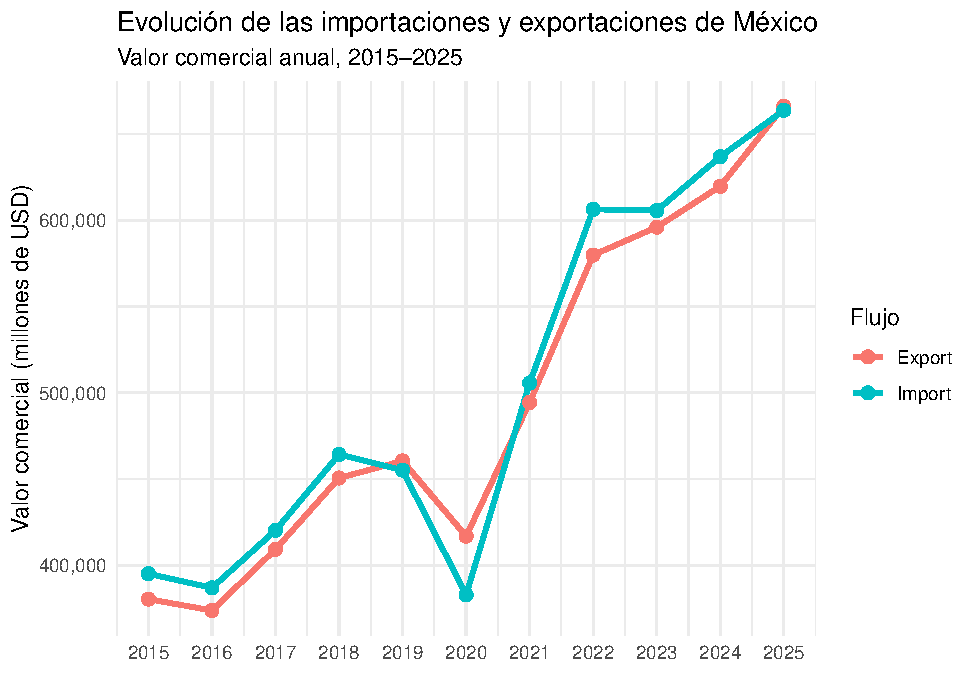
\includegraphics{Proyecto_9_EDA_files/Proyecto_9_EDA_files/figure-latex/unnamed-chunk-2-1.pdf}

A partir de la gráfica se observa una tendencia general de crecimiento
del valor nominal entre 2015 y 2025, aunque no de forma continua. En
2020 se presenta una disminución tanto en importaciones como en
exportaciones respecto de 2019, coincidiendo con el periodo de
disrupciones internacionales asociado a la pandemia de COVID-19. A
partir de 2021 ambos flujos muestran una recuperación y alcanzan sus
mayores valores hacia el final del periodo.

Dado que los valores están expresados en USD corrientes, este
comportamiento describe la evolución del valor monetario reportado y no
debe interpretarse directamente como crecimiento del volumen físico
comerciado.

El siguiente paso consiste en analizar los principales socios del
comercio mexicano.

\textbf{Principales socios comerciales}

Las siguientes tablas muestran los cinco principales socios de México en
exportaciones e importaciones de acuerdo con el valor comercial
acumulado nominal durante el periodo analizado.

\emph{IMPORTACIONES}

\begin{verbatim}
## # A tibble: 5 x 3
##   partnerDesc   total_valor_M_usd porcentaje
##   <chr>         <chr>             <chr>     
## 1 USA           2,415,479         43.7%     
## 2 China         1,050,837         19.0%     
## 3 Rep. of Korea 200,044           3.6%      
## 4 Japan         197,230           3.6%      
## 5 Germany       191,401           3.5%
\end{verbatim}

\emph{EXPORTACIONES}

\begin{verbatim}
## # A tibble: 5 x 3
##   partnerDesc                            total_valor_M_usd porcentaje
##   <chr>                                  <chr>             <chr>     
## 1 USA                                    4,349,854         79.8%     
## 2 Canada                                 158,277           2.9%      
## 3 China                                  87,066            1.6%      
## 4 Germany                                74,722            1.4%      
## 5 North America and Central America, nes 61,706            1.1%
\end{verbatim}

Los resultados permiten identificar a los países que concentraron los
mayores valores comerciales acumulados durante 2015--2025. En
particular, Estados Unidos ocupa una posición predominante tanto como
destino de las exportaciones mexicanas como entre los proveedores de las
importaciones.

Veamos si a lo largo del tiempo estos 5 socios han cambiado.

\textbf{Evolución de la participación de los principales socios}

Para cada año se calcula la proporción del valor importado
correspondiente al proveedor principal (Top 1) y a los tres principales
proveedores en conjunto (Top 3).

\emph{IMPORTACIONES}
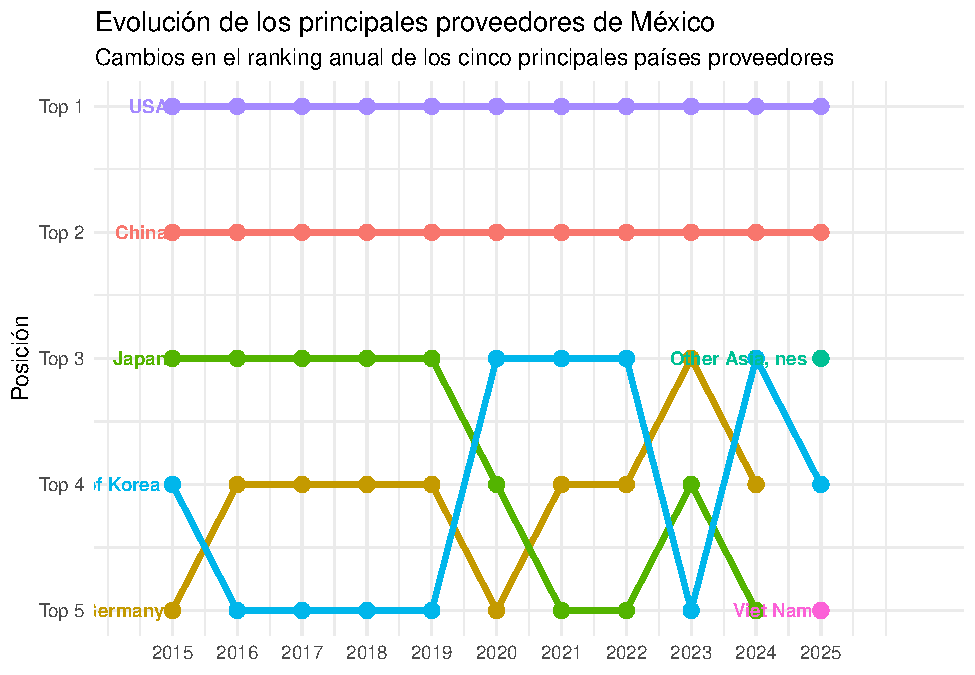
\includegraphics{Proyecto_9_EDA_files/Proyecto_9_EDA_files/figure-latex/unnamed-chunk-5-1.pdf}
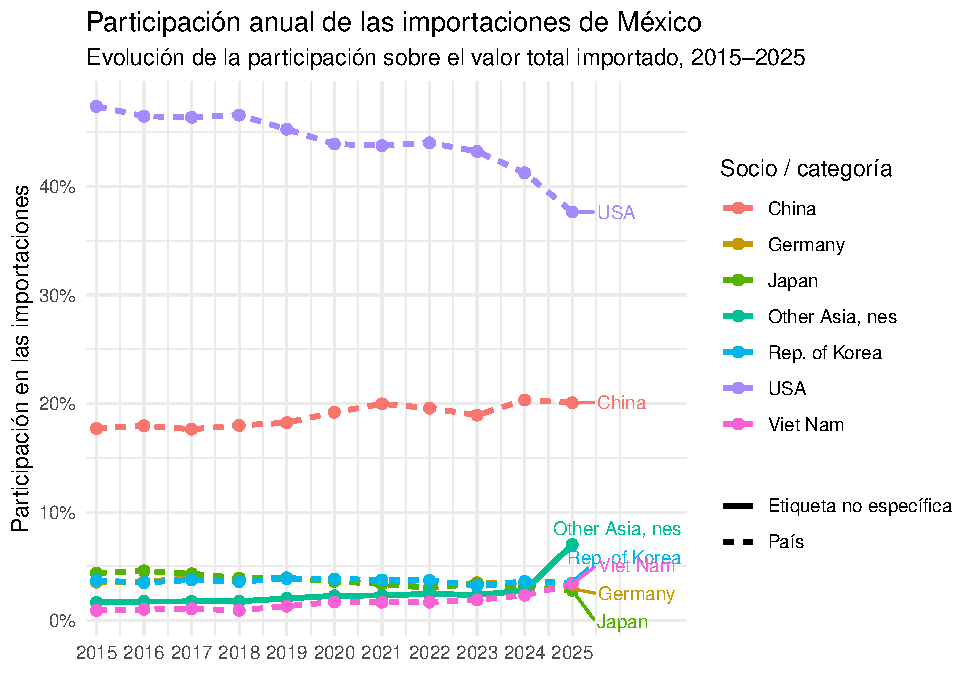
\includegraphics{Proyecto_9_EDA_files/Proyecto_9_EDA_files/figure-latex/unnamed-chunk-5-2.pdf}

Las dos visualizaciones muestran que la estructura de los principales
proveedores de México Estados Unidos se mantiene como el principal
proveedor durante todo el periodo 2015--2025 y China conserva el segundo
lugar. No obstante, la participación de Estados Unidos disminuye
gradualmente, mientras que la de China permanece relativamente estable e
incluso aumenta ligeramente hacia los últimos años.

A partir del tercer lugar se observa una mayor rotación. Japón,
República de Corea y Alemania intercambian posiciones durante buena
parte del periodo, mientras que hacia los años más recientes aparecen
nuevos cambios en la composición de los principales proveedores. En
particular, en 2025 destaca el incremento de Other Asia, nes y la
presencia de Viet Nam entre los proveedores de mayor participación.

El aumento reciente de la participación de proveedores asiáticos podría
estar relacionado con una reconfiguración de las cadenas de suministro
internacionales posterior a las tensiones comerciales entre Estados
Unidos y China. En particular, los aranceles aplicados a productos
chinos desde 2018 y las medidas posteriores sobre sectores tecnológicos
pudieron generar incentivos para diversificar proveedores y relocalizar
etapas de producción hacia México y otros países asiáticos.

\emph{EXPORTACIONES}
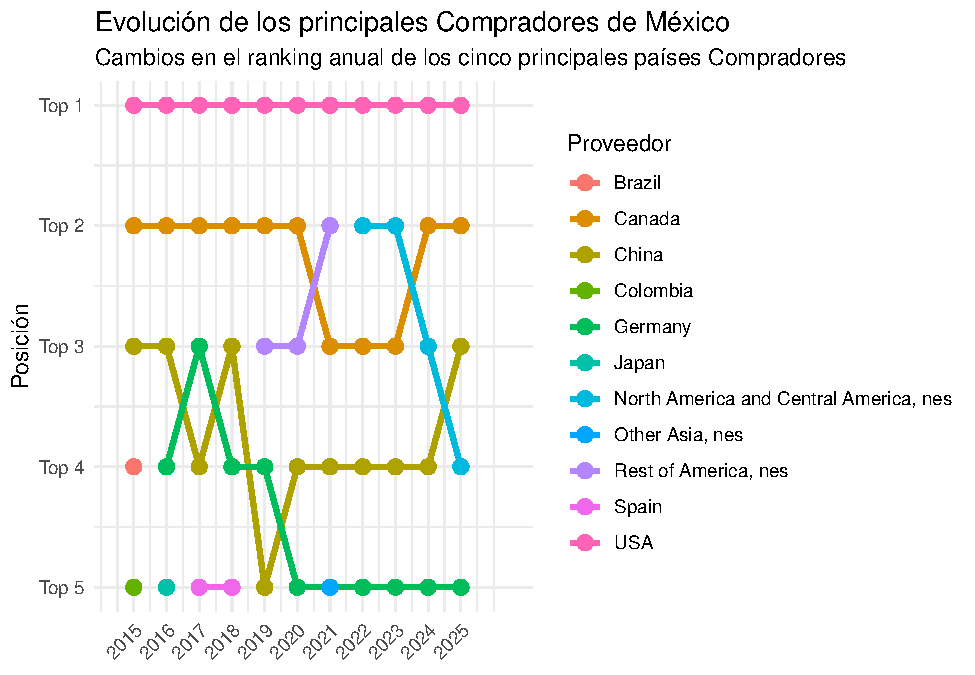
\includegraphics{Proyecto_9_EDA_files/Proyecto_9_EDA_files/figure-latex/unnamed-chunk-6-1.pdf}
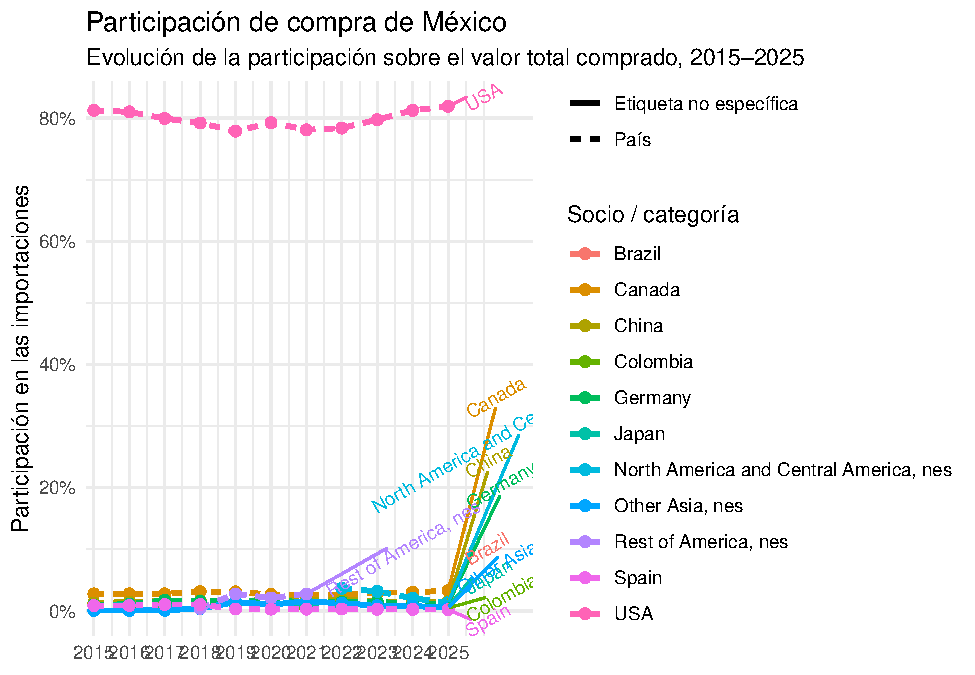
\includegraphics{Proyecto_9_EDA_files/Proyecto_9_EDA_files/figure-latex/unnamed-chunk-6-2.pdf}

En las exportaciones se observa que Estados Unidos se mantiene en la
primera posición durante todo el periodo 2015--2025 y concentra una
proporción ampliamente superior a la del resto de los compradores.A
partir de la segunda posición existe una mayor movilidad.

El análisis muestra diferencias entre la estructura de las importaciones
y exportaciones. Sin embargo, esta visión puede ocultar comportamientos
distintos entre categorías de productos. Un capítulo HS2 puede
concentrar gran parte de su comercio en un solo socio, mientras que otro
puede distribuirlo entre numerosos países.

Por ello, el siguiente paso consiste en medir la concentración de socios
dentro de cada capítulo HS2 y para cada año, con especial atención a las
importaciones, que constituyen el foco principal del análisis.

Para cada año, flujo y capítulo, la participación del socio es
\(p_i = valor_i / \sum_j valor_j\). El índice de Herfindahl--Hirschman
es \(HHI = \sum_i p_i^2\). Cercano a 1 implica mayor concentración de
\textbf{valor}; el número efectivo de socios es \(1/HHI\). \texttt{top1}
mide la cuota del socio principal. Los socios sin valor positivo
observado no se imputan como cero.Adicionalmente, se calcula
participacion, que representa el peso de cada capítulo HS2 dentro del
valor total del flujo comercial correspondiente a cada año

\textbf{- ¿Cómo ha evolucionado la concentración de proveedores de los
distintos capítulos HS2 entre 2015 y 2025?}

El análisis muestra diferencias entre la estructura de las importaciones
. Sin embargo, esta visión puede ocultar comportamientos distintos entre
categorías de productos. Un capítulo HS2 puede concentrar gran parte de
su comercio en un solo socio, mientras que otro puede distribuirlo entre
numerosos países.

Por ello, el siguiente paso consiste en medir la concentración de socios
dentro de cada capítulo HS2 y para cada año, con especial atención a las
importaciones, que constituyen el foco principal del análisis.

Para cada año, flujo y capítulo, la participación del socio es
\(p_i = valor_i / \sum_j valor_j\). El índice de Herfindahl--Hirschman
es \(HHI = \sum_i p_i^2\). Cercano a 1 implica mayor concentración de
\textbf{valor}; el número efectivo de socios es \(1/HHI\). \texttt{top1}
mide la cuota del socio principal. Los socios sin valor positivo
observado no se imputan como cero.Adicionalmente, se calcula
participacion, que representa el peso de cada capítulo HS2 dentro del
valor total del flujo comercial correspondiente a cada año

Como primera aproximación, se examinan los capítulos de importación con
mayor concentración en 2025. Esta comparación permite identificar qué
categorías presentan valores elevados de HHI y determinar si dicha
concentración corresponde además a capítulos de importancia económica
relevante.

\begin{longtable}[]{@{}
  >{\raggedright\arraybackslash}p{(\columnwidth - 12\tabcolsep) * \real{0.0204}}
  >{\raggedright\arraybackslash}p{(\columnwidth - 12\tabcolsep) * \real{0.5765}}
  >{\raggedleft\arraybackslash}p{(\columnwidth - 12\tabcolsep) * \real{0.0714}}
  >{\raggedleft\arraybackslash}p{(\columnwidth - 12\tabcolsep) * \real{0.0765}}
  >{\raggedleft\arraybackslash}p{(\columnwidth - 12\tabcolsep) * \real{0.0306}}
  >{\raggedleft\arraybackslash}p{(\columnwidth - 12\tabcolsep) * \real{0.1224}}
  >{\raggedright\arraybackslash}p{(\columnwidth - 12\tabcolsep) * \real{0.1020}}@{}}
\caption{Diez capítulos HS2 con mayor concentración de proveedores en
2025}\tabularnewline
\toprule\noalign{}
\begin{minipage}[b]{\linewidth}\raggedright
HS2
\end{minipage} & \begin{minipage}[b]{\linewidth}\raggedright
Capítulo
\end{minipage} & \begin{minipage}[b]{\linewidth}\raggedleft
Valor (M USD)
\end{minipage} & \begin{minipage}[b]{\linewidth}\raggedleft
Núm. de socios
\end{minipage} & \begin{minipage}[b]{\linewidth}\raggedleft
HHI
\end{minipage} & \begin{minipage}[b]{\linewidth}\raggedleft
Proveedor principal (\%)
\end{minipage} & \begin{minipage}[b]{\linewidth}\raggedright
Proveedor principal
\end{minipage} \\
\midrule\noalign{}
\endfirsthead
\toprule\noalign{}
\begin{minipage}[b]{\linewidth}\raggedright
HS2
\end{minipage} & \begin{minipage}[b]{\linewidth}\raggedright
Capítulo
\end{minipage} & \begin{minipage}[b]{\linewidth}\raggedleft
Valor (M USD)
\end{minipage} & \begin{minipage}[b]{\linewidth}\raggedleft
Núm. de socios
\end{minipage} & \begin{minipage}[b]{\linewidth}\raggedleft
HHI
\end{minipage} & \begin{minipage}[b]{\linewidth}\raggedleft
Proveedor principal (\%)
\end{minipage} & \begin{minipage}[b]{\linewidth}\raggedright
Proveedor principal
\end{minipage} \\
\midrule\noalign{}
\endhead
\bottomrule\noalign{}
\endlastfoot
67 & Feathers and down, prepared; and articles made of feather or of
down; artificial flowers; articles of human hair & 92.9 & 15 & 0.917 &
95.7 & China \\
27 & Mineral fuels, mineral oils and products of their distillation;
bituminous substances; mineral waxes & 36,996.2 & 38 & 0.870 & 93.3 &
USA \\
10 & Cereals & 8,179.9 & 16 & 0.805 & 89.6 & USA \\
66 & Umbrellas, sun umbrellas, walking-sticks, seat sticks, whips,
riding crops; and parts thereof & 57.6 & 13 & 0.743 & 85.6 & China \\
23 & Food industries, residues and wastes thereof; prepared animal
fodder & 2,400.1 & 23 & 0.741 & 85.9 & USA \\
04 & Dairy produce; birds' eggs; natural honey; edible products of
animal origin, not elsewhere specified or included & 3,149.4 & 18 &
0.678 & 81.9 & USA \\
17 & Sugars and sugar confectionery & 1,333.0 & 32 & 0.666 & 80.9 &
USA \\
50 & Silk & 7.2 & 7 & 0.606 & 74.4 & China \\
05 & Animal originated products; not elsewhere specified or included &
368.2 & 12 & 0.570 & 74.3 & USA \\
21 & Miscellaneous edible preparations & 2,694.6 & 50 & 0.564 & 74.8 &
USA \\
\end{longtable}

\subsubsection{Hallazgos principales: concentración de importaciones en
2025}\label{hallazgos-principales-concentraciuxf3n-de-importaciones-en-2025}

\begin{itemize}
\tightlist
\item
  \textbf{Combustibles y aceites minerales (HS2 \texttt{27}) combinan
  valor elevado y alta concentración:} México importó aproximadamente
  \textbf{37,000 millones de USD} y \textbf{93.3\%} del valor provino de
  USA.
\item
  \textbf{Cereales (HS2 \texttt{10}) muestran un patrón similar:} el
  valor importado fue de aproximadamente \textbf{8,180 millones de USD},
  con \textbf{89.6\%} procedente de USA.
\item
  \textbf{Plumas y artículos relacionados (HS2 \texttt{67}) tienen el
  HHI más alto}, pero su valor importado fue mucho menor (\textbf{92.9
  millones de USD}). Por ello, la concentración debe interpretarse junto
  con la importancia económica del capítulo.
\item
  \textbf{Contar países no basta para medir diversificación:} en
  preparaciones alimenticias diversas (HS2 \texttt{21}) aparecen
  \textbf{50 socios}, pero USA concentra \textbf{74.8\%} del valor.
\end{itemize}

Entre los capítulos mostrados, \texttt{27} y \texttt{10} destacan por
combinar valores importados elevados con una fuerte concentración en un
socio. Estos resultados describen el \textbf{valor comercial registrado
en 2025}; por sí solos no miden cantidades físicas ni riesgo de
desabasto.

\begin{longtable}[]{@{}
  >{\raggedright\arraybackslash}p{(\columnwidth - 12\tabcolsep) * \real{0.0135}}
  >{\raggedright\arraybackslash}p{(\columnwidth - 12\tabcolsep) * \real{0.7196}}
  >{\raggedleft\arraybackslash}p{(\columnwidth - 12\tabcolsep) * \real{0.0473}}
  >{\raggedleft\arraybackslash}p{(\columnwidth - 12\tabcolsep) * \real{0.0507}}
  >{\raggedleft\arraybackslash}p{(\columnwidth - 12\tabcolsep) * \real{0.0203}}
  >{\raggedleft\arraybackslash}p{(\columnwidth - 12\tabcolsep) * \real{0.0811}}
  >{\raggedright\arraybackslash}p{(\columnwidth - 12\tabcolsep) * \real{0.0676}}@{}}
\caption{Diez capítulos HS2 con mayor concentración de proveedores en
2015}\tabularnewline
\toprule\noalign{}
\begin{minipage}[b]{\linewidth}\raggedright
HS2
\end{minipage} & \begin{minipage}[b]{\linewidth}\raggedright
Capítulo
\end{minipage} & \begin{minipage}[b]{\linewidth}\raggedleft
Valor (M USD)
\end{minipage} & \begin{minipage}[b]{\linewidth}\raggedleft
Núm. de socios
\end{minipage} & \begin{minipage}[b]{\linewidth}\raggedleft
HHI
\end{minipage} & \begin{minipage}[b]{\linewidth}\raggedleft
Proveedor principal (\%)
\end{minipage} & \begin{minipage}[b]{\linewidth}\raggedright
Proveedor principal
\end{minipage} \\
\midrule\noalign{}
\endfirsthead
\toprule\noalign{}
\begin{minipage}[b]{\linewidth}\raggedright
HS2
\end{minipage} & \begin{minipage}[b]{\linewidth}\raggedright
Capítulo
\end{minipage} & \begin{minipage}[b]{\linewidth}\raggedleft
Valor (M USD)
\end{minipage} & \begin{minipage}[b]{\linewidth}\raggedleft
Núm. de socios
\end{minipage} & \begin{minipage}[b]{\linewidth}\raggedleft
HHI
\end{minipage} & \begin{minipage}[b]{\linewidth}\raggedleft
Proveedor principal (\%)
\end{minipage} & \begin{minipage}[b]{\linewidth}\raggedright
Proveedor principal
\end{minipage} \\
\midrule\noalign{}
\endhead
\bottomrule\noalign{}
\endlastfoot
23 & Food industries, residues and wastes thereof; prepared animal
fodder & 1,623.3 & 23 & 0.870 & 93.2 & USA \\
66 & Umbrellas, sun umbrellas, walking-sticks, seat sticks, whips,
riding crops; and parts thereof & 46.5 & 24 & 0.808 & 89.6 & China \\
17 & Sugars and sugar confectionery & 807.0 & 48 & 0.790 & 88.8 & USA \\
05 & Animal originated products; not elsewhere specified or included &
274.1 & 20 & 0.763 & 86.9 & USA \\
10 & Cereals & 4,005.4 & 20 & 0.758 & 86.8 & USA \\
27 & Mineral fuels, mineral oils and products of their distillation;
bituminous substances; mineral waxes & 26,455.5 & 58 & 0.715 & 84.2 &
USA \\
67 & Feathers and down, prepared; and articles made of feather or of
down; artificial flowers; articles of human hair & 45.8 & 24 & 0.695 &
83.0 & China \\
21 & Miscellaneous edible preparations & 1,324.1 & 57 & 0.693 & 83.1 &
USA \\
86 & Railway, tramway locomotives, rolling-stock and parts thereof;
railway or tramway track fixtures and fittings and parts thereof;
mechanical (including electro-mechanical) traffic signalling equipment
of all kinds & 1,464.8 & 32 & 0.692 & 82.7 & USA \\
02 & Meat and edible meat offal & 3,820.5 & 14 & 0.691 & 82.5 & USA \\
\end{longtable}

\subsubsection{Hallazgos relevantes: concentración de importaciones en
2015}\label{hallazgos-relevantes-concentraciuxf3n-de-importaciones-en-2015}

\begin{itemize}
\item
  \textbf{Combustibles minerales (HS2 \texttt{27}) combinó valor elevado
  y concentración:} México importó aproximadamente \textbf{26,456
  millones de USD} y \textbf{84.2\%} del valor provino de USA. Fue el
  capítulo de mayor valor entre los diez con HHI más alto.
\item
  \textbf{Residuos de la industria alimentaria y forraje (HS2
  \texttt{23}) fue el más concentrado de los diez:} registró un HHI de
  \textbf{0.870} y USA aportó \textbf{93.2\%} de los aproximadamente
  \textbf{1,623 millones de USD} importados.
\item
  \textbf{Un número alto de socios no garantiza que el valor esté
  repartido:} en preparaciones alimenticias diversas (HS2 \texttt{21})
  aparecen \textbf{57 países}, pero USA concentró \textbf{83.1\%} del
  valor.
\item
  \textbf{USA fue el socio principal en ocho de los diez capítulos} con
  mayor HHI. China fue el socio principal en los capítulos \texttt{66} y
  \texttt{67}, que también mostraron alta concentración, aunque con
  valores importados mucho menores.
\end{itemize}

Veamos su cambio de 2015 a 2025

\begin{longtable}[]{@{}
  >{\raggedright\arraybackslash}p{(\columnwidth - 18\tabcolsep) * \real{0.0179}}
  >{\raggedright\arraybackslash}p{(\columnwidth - 18\tabcolsep) * \real{0.5045}}
  >{\raggedleft\arraybackslash}p{(\columnwidth - 18\tabcolsep) * \real{0.0402}}
  >{\raggedleft\arraybackslash}p{(\columnwidth - 18\tabcolsep) * \real{0.0402}}
  >{\raggedleft\arraybackslash}p{(\columnwidth - 18\tabcolsep) * \real{0.0491}}
  >{\raggedleft\arraybackslash}p{(\columnwidth - 18\tabcolsep) * \real{0.0670}}
  >{\raggedleft\arraybackslash}p{(\columnwidth - 18\tabcolsep) * \real{0.0670}}
  >{\raggedleft\arraybackslash}p{(\columnwidth - 18\tabcolsep) * \real{0.0804}}
  >{\raggedright\arraybackslash}p{(\columnwidth - 18\tabcolsep) * \real{0.0670}}
  >{\raggedright\arraybackslash}p{(\columnwidth - 18\tabcolsep) * \real{0.0670}}@{}}
\caption{Capítulos con mayor aumento en la concentración de proveedores
entre 2015 y 2025}\tabularnewline
\toprule\noalign{}
\begin{minipage}[b]{\linewidth}\raggedright
HS2
\end{minipage} & \begin{minipage}[b]{\linewidth}\raggedright
Capítulo
\end{minipage} & \begin{minipage}[b]{\linewidth}\raggedleft
HHI 2015
\end{minipage} & \begin{minipage}[b]{\linewidth}\raggedleft
HHI 2025
\end{minipage} & \begin{minipage}[b]{\linewidth}\raggedleft
Cambio HHI
\end{minipage} & \begin{minipage}[b]{\linewidth}\raggedleft
Top 1 2015 (\%)
\end{minipage} & \begin{minipage}[b]{\linewidth}\raggedleft
Top 1 2025 (\%)
\end{minipage} & \begin{minipage}[b]{\linewidth}\raggedleft
Cambio Top 1 (pp)
\end{minipage} & \begin{minipage}[b]{\linewidth}\raggedright
Proveedor 2015
\end{minipage} & \begin{minipage}[b]{\linewidth}\raggedright
Proveedor 2025
\end{minipage} \\
\midrule\noalign{}
\endfirsthead
\toprule\noalign{}
\begin{minipage}[b]{\linewidth}\raggedright
HS2
\end{minipage} & \begin{minipage}[b]{\linewidth}\raggedright
Capítulo
\end{minipage} & \begin{minipage}[b]{\linewidth}\raggedleft
HHI 2015
\end{minipage} & \begin{minipage}[b]{\linewidth}\raggedleft
HHI 2025
\end{minipage} & \begin{minipage}[b]{\linewidth}\raggedleft
Cambio HHI
\end{minipage} & \begin{minipage}[b]{\linewidth}\raggedleft
Top 1 2015 (\%)
\end{minipage} & \begin{minipage}[b]{\linewidth}\raggedleft
Top 1 2025 (\%)
\end{minipage} & \begin{minipage}[b]{\linewidth}\raggedleft
Cambio Top 1 (pp)
\end{minipage} & \begin{minipage}[b]{\linewidth}\raggedright
Proveedor 2015
\end{minipage} & \begin{minipage}[b]{\linewidth}\raggedright
Proveedor 2025
\end{minipage} \\
\midrule\noalign{}
\endhead
\bottomrule\noalign{}
\endlastfoot
50 & Silk & 0.193 & 0.606 & 0.413 & 31.0 & 74.4 & 43.3 & China &
China \\
14 & Vegetable plaiting materials; vegetable products not elsewhere
specified or included & 0.190 & 0.469 & 0.280 & 26.9 & 66.4 & 39.6 &
Peru & Sri Lanka \\
93 & Arms and ammunition; parts and accessories thereof & 0.156 & 0.394
& 0.238 & 27.6 & 55.0 & 27.4 & USA & Areas, nes \\
67 & Feathers and down, prepared; and articles made of feather or of
down; artificial flowers; articles of human hair & 0.695 & 0.917 & 0.222
& 83.0 & 95.7 & 12.7 & China & China \\
89 & Ships, boats and floating structures & 0.294 & 0.508 & 0.214 & 46.9
& 67.3 & 20.4 & Spain & USA \\
26 & Ores, slag and ash & 0.219 & 0.430 & 0.211 & 42.4 & 61.1 & 18.7 &
USA & USA \\
91 & Clocks and watches and parts thereof & 0.364 & 0.550 & 0.186 & 45.5
& 72.4 & 27.0 & Switzerland & Switzerland \\
27 & Mineral fuels, mineral oils and products of their distillation;
bituminous substances; mineral waxes & 0.715 & 0.870 & 0.156 & 84.2 &
93.3 & 9.1 & USA & USA \\
75 & Nickel and articles thereof & 0.315 & 0.451 & 0.136 & 53.3 & 66.4 &
13.0 & USA & USA \\
53 & Vegetable textile fibres; paper yarn and woven fabrics of paper
yarn & 0.183 & 0.294 & 0.111 & 35.0 & 51.1 & 16.1 & Sri Lanka & China \\
\end{longtable}

Al comparar 2015 con 2025 se observa que el aumento de la concentración
de proveedores no ocurrió de la misma manera en todos los capítulos. En
algunos casos, el proveedor principal se mantuvo sin cambios pero
incrementó considerablemente su participación. Por ejemplo, en seda
(HS50) China pasó de concentrar 31.0\% a 74.4\% del valor importado,
mientras que el HHI aumentó de 0.193 a 0.606.

En otros capítulos, el aumento de la concentración estuvo acompañado por
un cambio en el proveedor principal. En materias vegetales para trenzar
(HS14) el liderazgo pasó de Perú a Sri Lanka y la participación del
principal proveedor aumentó de 26.9\% a 66.4\%.

En conjunto, estos resultados muestran que el incremento del HHI puede
responder tanto al fortalecimiento de un proveedor que ya era dominante
como a una reconfiguración del proveedor principal.

\emph{Ahora cuales se diversificaron}

\begin{longtable}[]{@{}
  >{\raggedright\arraybackslash}p{(\columnwidth - 18\tabcolsep) * \real{0.0150}}
  >{\raggedright\arraybackslash}p{(\columnwidth - 18\tabcolsep) * \real{0.5843}}
  >{\raggedleft\arraybackslash}p{(\columnwidth - 18\tabcolsep) * \real{0.0337}}
  >{\raggedleft\arraybackslash}p{(\columnwidth - 18\tabcolsep) * \real{0.0337}}
  >{\raggedleft\arraybackslash}p{(\columnwidth - 18\tabcolsep) * \real{0.0412}}
  >{\raggedleft\arraybackslash}p{(\columnwidth - 18\tabcolsep) * \real{0.0562}}
  >{\raggedleft\arraybackslash}p{(\columnwidth - 18\tabcolsep) * \real{0.0562}}
  >{\raggedleft\arraybackslash}p{(\columnwidth - 18\tabcolsep) * \real{0.0674}}
  >{\raggedright\arraybackslash}p{(\columnwidth - 18\tabcolsep) * \real{0.0562}}
  >{\raggedright\arraybackslash}p{(\columnwidth - 18\tabcolsep) * \real{0.0562}}@{}}
\caption{Capítulos con mayor reducción en la concentración de
proveedores entre 2015 y 2025}\tabularnewline
\toprule\noalign{}
\begin{minipage}[b]{\linewidth}\raggedright
HS2
\end{minipage} & \begin{minipage}[b]{\linewidth}\raggedright
Capítulo
\end{minipage} & \begin{minipage}[b]{\linewidth}\raggedleft
HHI 2015
\end{minipage} & \begin{minipage}[b]{\linewidth}\raggedleft
HHI 2025
\end{minipage} & \begin{minipage}[b]{\linewidth}\raggedleft
Cambio HHI
\end{minipage} & \begin{minipage}[b]{\linewidth}\raggedleft
Top 1 2015 (\%)
\end{minipage} & \begin{minipage}[b]{\linewidth}\raggedleft
Top 1 2025 (\%)
\end{minipage} & \begin{minipage}[b]{\linewidth}\raggedleft
Cambio Top 1 (pp)
\end{minipage} & \begin{minipage}[b]{\linewidth}\raggedright
Proveedor 2015
\end{minipage} & \begin{minipage}[b]{\linewidth}\raggedright
Proveedor 2025
\end{minipage} \\
\midrule\noalign{}
\endfirsthead
\toprule\noalign{}
\begin{minipage}[b]{\linewidth}\raggedright
HS2
\end{minipage} & \begin{minipage}[b]{\linewidth}\raggedright
Capítulo
\end{minipage} & \begin{minipage}[b]{\linewidth}\raggedleft
HHI 2015
\end{minipage} & \begin{minipage}[b]{\linewidth}\raggedleft
HHI 2025
\end{minipage} & \begin{minipage}[b]{\linewidth}\raggedleft
Cambio HHI
\end{minipage} & \begin{minipage}[b]{\linewidth}\raggedleft
Top 1 2015 (\%)
\end{minipage} & \begin{minipage}[b]{\linewidth}\raggedleft
Top 1 2025 (\%)
\end{minipage} & \begin{minipage}[b]{\linewidth}\raggedleft
Cambio Top 1 (pp)
\end{minipage} & \begin{minipage}[b]{\linewidth}\raggedright
Proveedor 2015
\end{minipage} & \begin{minipage}[b]{\linewidth}\raggedright
Proveedor 2025
\end{minipage} \\
\midrule\noalign{}
\endhead
\bottomrule\noalign{}
\endlastfoot
59 & Textile fabrics; impregnated, coated, covered or laminated; textile
articles of a kind suitable for industrial use & 0.595 & 0.274 & -0.321
& 76.6 & 48.5 & -28.0 & USA & USA \\
57 & Carpets and other textile floor coverings & 0.536 & 0.241 & -0.295
& 72.4 & 42.2 & -30.1 & USA & USA \\
56 & Wadding, felt and nonwovens, special yarns; twine, cordage, ropes
and cables and articles thereof & 0.579 & 0.328 & -0.251 & 75.6 & 53.7 &
-22.0 & USA & USA \\
71 & Natural, cultured pearls; precious, semi-precious stones; precious
metals, metals clad with precious metal, and articles thereof; imitation
jewellery; coin & 0.396 & 0.153 & -0.244 & 61.4 & 29.9 & -31.5 & USA &
USA \\
79 & Zinc and articles thereof & 0.493 & 0.263 & -0.231 & 67.7 & 39.1 &
-28.6 & USA & USA \\
02 & Meat and edible meat offal & 0.691 & 0.479 & -0.212 & 82.5 & 65.9 &
-16.5 & USA & USA \\
11 & Products of the milling industry; malt, starches, inulin, wheat
gluten & 0.599 & 0.387 & -0.212 & 76.4 & 60.0 & -16.3 & USA & USA \\
37 & Photographic or cinematographic goods & 0.471 & 0.260 & -0.211 &
67.1 & 45.7 & -21.4 & USA & USA \\
95 & Toys, games and sports requisites; parts and accessories thereof &
0.552 & 0.349 & -0.203 & 73.4 & 56.0 & -17.4 & China & China \\
05 & Animal originated products; not elsewhere specified or included &
0.763 & 0.570 & -0.193 & 86.9 & 74.3 & -12.6 & USA & USA \\
\end{longtable}

Entre los capítulos que más redujeron su concentración entre 2015 y 2025
se observa un patrón consistente: en la mayoría de los casos el
proveedor principal se mantiene sin cambios, pero su participación
disminuye de forma importante. Esto sugiere que la diversificación
ocurrió principalmente por una redistribución del valor importado hacia
otros proveedores, más que por un reemplazo del país líder.

Por ejemplo, en tejidos textiles impregnados o recubiertos (HS59)
Estados Unidos continuó siendo el principal proveedor, pero su
participación cayó de 76.6\% a 48.5\%, mientras que el HHI disminuyó de
0.595 a 0.274.

En conjunto, el análisis muestra que la concentración de proveedores no
evolucionó de manera uniforme entre los distintos capítulos HS2. Algunos
capítulos aumentaron claramente su dependencia de pocos proveedores. En
otros casos ocurrió el proceso contrario: el HHI disminuyó y la
participación del proveedor principal se redujo, reflejando una
distribución más equilibrada del valor entre distintos socios.

Por lo tanto, para evaluar la estructura de proveedores no basta con
identificar al socio principal o contar el número de países
participantes. Es necesario considerar conjuntamente el HHI, la
participación del proveedor dominante y los cambios de estas medidas a
lo largo del tiempo.

Un capítulo altamente concentrado no necesariamente representa una parte
importante de las importaciones mexicanas. El siguiente paso consiste en
incorporar la importancia económica de cada capítulo para distinguir
entre casos de alta concentración pero bajo peso comercial y aquellos
que combinan concentración elevada con una participación relevante
dentro de las importaciones.

\textbf{- ¿Cómo ha cambiado la importancia económica de los distintos
capítulos HS2 dentro de las importaciones mexicanas durante el periodo
analizado?}

Después de analizar cómo ha cambiado la concentración de proveedores, el
siguiente paso consiste en evaluar la importancia económica de los
distintos capítulos HS2 dentro de las importaciones mexicanas.

\begin{longtable}[]{@{}
  >{\raggedright\arraybackslash}p{(\columnwidth - 4\tabcolsep) * \real{0.0537}}
  >{\raggedright\arraybackslash}p{(\columnwidth - 4\tabcolsep) * \real{0.8780}}
  >{\raggedleft\arraybackslash}p{(\columnwidth - 4\tabcolsep) * \real{0.0683}}@{}}
\caption{Principales capítulos HS2 exportados de México hacia Estados
Unidos, 2015--2025}\tabularnewline
\toprule\noalign{}
\begin{minipage}[b]{\linewidth}\raggedright
Código HS2
\end{minipage} & \begin{minipage}[b]{\linewidth}\raggedright
Producto
\end{minipage} & \begin{minipage}[b]{\linewidth}\raggedleft
Valor (M USD)
\end{minipage} \\
\midrule\noalign{}
\endfirsthead
\toprule\noalign{}
\begin{minipage}[b]{\linewidth}\raggedright
Código HS2
\end{minipage} & \begin{minipage}[b]{\linewidth}\raggedright
Producto
\end{minipage} & \begin{minipage}[b]{\linewidth}\raggedleft
Valor (M USD)
\end{minipage} \\
\midrule\noalign{}
\endhead
\bottomrule\noalign{}
\endlastfoot
87 & Vehicles; other than railway or tramway rolling stock, and parts
and accessories thereof & 1,110,594.5 \\
85 & Electrical machinery and equipment and parts thereof; sound
recorders and reproducers; television image and sound recorders and
reproducers, parts and accessories of such articles & 860,008.1 \\
84 & Nuclear reactors, boilers, machinery and mechanical appliances;
parts thereof & 439,763.5 \\
84 & Machinery and mechanical appliances, boilers, nuclear reactors;
parts thereof & 414,395.2 \\
90 & Optical, photographic, cinematographic, measuring, checking,
medical or surgical instruments and apparatus; parts and accessories &
219,553.4 \\
\end{longtable}

\begin{longtable}[]{@{}
  >{\raggedright\arraybackslash}p{(\columnwidth - 4\tabcolsep) * \real{0.0537}}
  >{\raggedright\arraybackslash}p{(\columnwidth - 4\tabcolsep) * \real{0.8780}}
  >{\raggedleft\arraybackslash}p{(\columnwidth - 4\tabcolsep) * \real{0.0683}}@{}}
\caption{Principales capítulos HS2 importados por México desde Estados
Unidos, 2015--2025}\tabularnewline
\toprule\noalign{}
\begin{minipage}[b]{\linewidth}\raggedright
Código HS2
\end{minipage} & \begin{minipage}[b]{\linewidth}\raggedright
Producto
\end{minipage} & \begin{minipage}[b]{\linewidth}\raggedleft
Valor (M USD)
\end{minipage} \\
\midrule\noalign{}
\endfirsthead
\toprule\noalign{}
\begin{minipage}[b]{\linewidth}\raggedright
Código HS2
\end{minipage} & \begin{minipage}[b]{\linewidth}\raggedright
Producto
\end{minipage} & \begin{minipage}[b]{\linewidth}\raggedleft
Valor (M USD)
\end{minipage} \\
\midrule\noalign{}
\endhead
\bottomrule\noalign{}
\endlastfoot
27 & Mineral fuels, mineral oils and products of their distillation;
bituminous substances; mineral waxes & 389,696.1 \\
85 & Electrical machinery and equipment and parts thereof; sound
recorders and reproducers; television image and sound recorders and
reproducers, parts and accessories of such articles & 252,271.8 \\
87 & Vehicles; other than railway or tramway rolling stock, and parts
and accessories thereof & 230,997.0 \\
39 & Plastics and articles thereof & 189,237.4 \\
84 & Nuclear reactors, boilers, machinery and mechanical appliances;
parts thereof & 186,704.7 \\
\end{longtable}

Notamos que con USA las categorías que se tienen en común tanto de
exportación como de importación son Vehículos, maquinaria eléctrica y
categoría 84 correspondiente a reactores nucleares, bolers, maquinaria y
partes para estos.

\emph{Exportaciones}

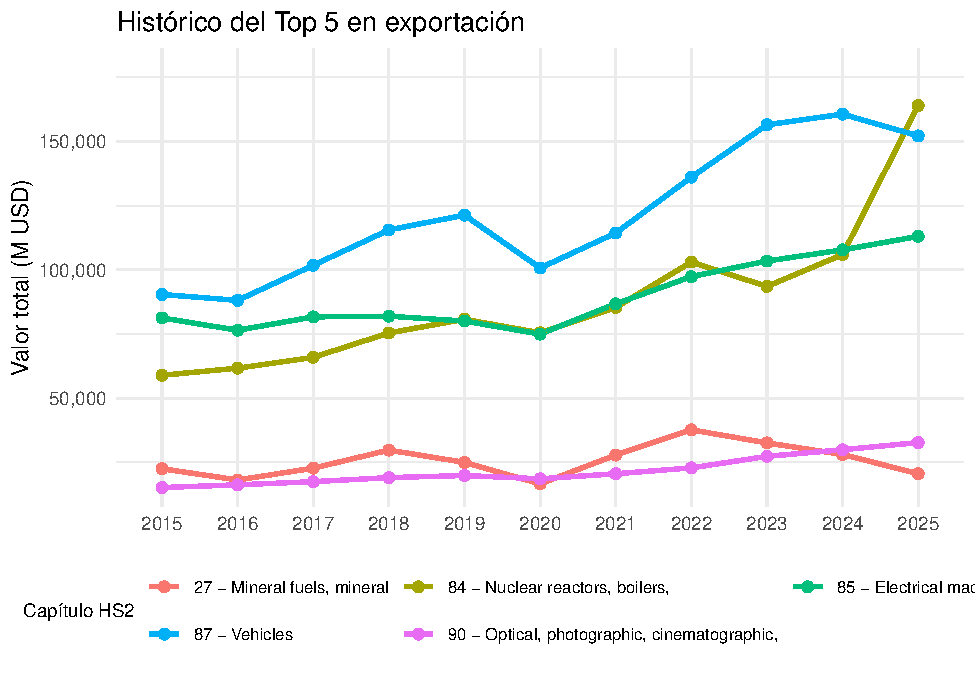
\includegraphics{Proyecto_9_EDA_files/Proyecto_9_EDA_files/figure-latex/unnamed-chunk-9-1.pdf}
Los cinco capítulos de mayor valor exportado acumulado presentan
trayectorias distintas durante 2015--2025. Vehículos (HS87) mantiene el
mayor valor exportado durante la mayor parte del periodo y muestra una
tendencia general creciente, aunque con una caída visible en 2020 y una
ligera reducción en 2025. Maquinaria mecánica (HS84) y maquinaria
eléctrica (HS85) también muestran una tendencia ascendente, destacando
el fuerte incremento de HS84 hacia 2025.

\emph{Importaciones}
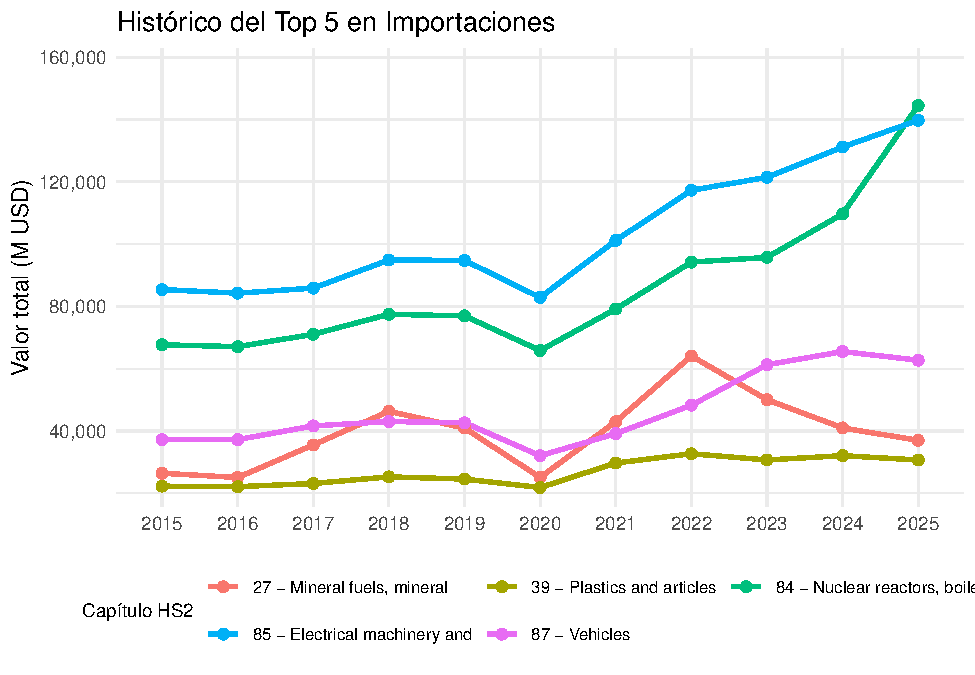
\includegraphics{Proyecto_9_EDA_files/Proyecto_9_EDA_files/figure-latex/unnamed-chunk-10-1.pdf}

Los principales capítulos de importación presentan diferencias
importantes tanto en su magnitud como en su evolución durante el
periodo. Maquinaria eléctrica (HS85) y maquinaria mecánica (HS84)
concentran los mayores valores importados, mientras que vehículos
(HS87), combustibles minerales (HS27) y plásticos (HS39) muestran
trayectorias menores.

Al igual que en las exportaciones, en 2020 se observa una caída en
varios de los principales capítulos, seguida de una recuperación
posterior. Sin embargo, dado que los valores están expresados en USD
corrientes, estas variaciones representan cambios en el valor monetario
importado y no necesariamente cambios equivalentes en las cantidades
físicas comerciadas.

El análisis exploratorio muestra que los capítulos HS2 no evolucionan de
manera homogénea. Algunos mantienen una participación elevada dentro de
las importaciones, otros ganan o pierden importancia a lo largo del
periodo y, al mismo tiempo, presentan distintos niveles y cambios en la
concentración de sus proveedores. Analizar cada capítulo de manera
individual permite identificar casos particulares, pero dificulta
reconocer patrones comunes entre el conjunto de categorías. Por ello, se
utiliza un modelo de agrupamiento K-Means con el objetivo de identificar
capítulos HS2 que presenten perfiles similares.

\begin{center}\rule{0.5\linewidth}{0.5pt}\end{center}

\subsection{Pregunta de investigación y alcance del
modelo}\label{pregunta-de-investigaciuxf3n-y-alcance-del-modelo}

\textbf{Pregunta principal:} ¿Es posible identificar grupos de capítulos
HS2 con perfiles similares de importancia económica y concentración de
proveedores, considerando tanto sus niveles como los cambios observados
entre el inicio y el final del periodo?

\textbf{Hipótesis descriptiva:} la concentración no cambia de la misma
manera en todos los capítulos, algunos de alto valor se concentran más y
otros se diversifican. Se describen asociaciones, sin atribuir los
cambios a una causa concreta.

La \textbf{unidad del EDA} es año × flujo × capítulo HS2 y, cuando se
estudian cuotas, socio comercial. El EDA conserva las etiquetas
originales; el modelo utiliza únicamente el valor asignado a socios
geográficos identificados. La \textbf{unidad de K-means} será el
capítulo HS2: cada capítulo tendrá indicadores resumidos de
concentración, cambio y participación importadora. No existe una
etiqueta futura a predecir; el HHI es el indicador principal que
queremos comprender y los grupos son perfiles descriptivos. Las
exportaciones se conservan como contexto de la relación comercial de
México, mientras que el modelo se enfoca en proveedores de
importaciones.

\subsubsection{1. Cobertura y calidad antes de comparar
años}\label{cobertura-y-calidad-antes-de-comparar-auxf1os}

El número de capítulos, socios y registros por año permite detectar
descargas incompletas. Revisar especialmente 2025 antes de interpretar
cambios. Un país o capítulo sin valor positivo registrado no se imputa
automáticamente como cero.

\begin{Shaded}
\begin{Highlighting}[]
\NormalTok{calidad\_adicional }\OtherTok{\textless{}{-}} \FunctionTok{tibble}\NormalTok{(}
  \AttributeTok{registros\_origen =} \FunctionTok{nrow}\NormalTok{(df\_comercio),}
  \AttributeTok{registros\_limpios =} \FunctionTok{nrow}\NormalTok{(df\_clean),}
  \AttributeTok{valor\_faltante\_origen =} \FunctionTok{sum}\NormalTok{(}\FunctionTok{is.na}\NormalTok{(df\_comercio}\SpecialCharTok{$}\NormalTok{primaryValue)),}
  \AttributeTok{valor\_no\_positivo\_origen =} \FunctionTok{sum}\NormalTok{(}\SpecialCharTok{!}\FunctionTok{is.na}\NormalTok{(df\_comercio}\SpecialCharTok{$}\NormalTok{primaryValue) }\SpecialCharTok{\&}
\NormalTok{                                   df\_comercio}\SpecialCharTok{$}\NormalTok{primaryValue }\SpecialCharTok{\textless{}=} \DecValTok{0}\NormalTok{),}
  \AttributeTok{duplicados\_exactos\_origen =} \FunctionTok{sum}\NormalTok{(}\FunctionTok{duplicated}\NormalTok{(df\_comercio))}
\NormalTok{)}
\NormalTok{knitr}\SpecialCharTok{::}\FunctionTok{kable}\NormalTok{(calidad\_adicional, }\AttributeTok{caption =} \StringTok{"Auditoría básica de calidad"}\NormalTok{)}
\end{Highlighting}
\end{Shaded}

\begin{longtable}[]{@{}
  >{\raggedleft\arraybackslash}p{(\columnwidth - 8\tabcolsep) * \real{0.1574}}
  >{\raggedleft\arraybackslash}p{(\columnwidth - 8\tabcolsep) * \real{0.1667}}
  >{\raggedleft\arraybackslash}p{(\columnwidth - 8\tabcolsep) * \real{0.2037}}
  >{\raggedleft\arraybackslash}p{(\columnwidth - 8\tabcolsep) * \real{0.2315}}
  >{\raggedleft\arraybackslash}p{(\columnwidth - 8\tabcolsep) * \real{0.2407}}@{}}
\caption{Auditoría básica de calidad}\tabularnewline
\toprule\noalign{}
\begin{minipage}[b]{\linewidth}\raggedleft
registros\_origen
\end{minipage} & \begin{minipage}[b]{\linewidth}\raggedleft
registros\_limpios
\end{minipage} & \begin{minipage}[b]{\linewidth}\raggedleft
valor\_faltante\_origen
\end{minipage} & \begin{minipage}[b]{\linewidth}\raggedleft
valor\_no\_positivo\_origen
\end{minipage} & \begin{minipage}[b]{\linewidth}\raggedleft
duplicados\_exactos\_origen
\end{minipage} \\
\midrule\noalign{}
\endfirsthead
\toprule\noalign{}
\begin{minipage}[b]{\linewidth}\raggedleft
registros\_origen
\end{minipage} & \begin{minipage}[b]{\linewidth}\raggedleft
registros\_limpios
\end{minipage} & \begin{minipage}[b]{\linewidth}\raggedleft
valor\_faltante\_origen
\end{minipage} & \begin{minipage}[b]{\linewidth}\raggedleft
valor\_no\_positivo\_origen
\end{minipage} & \begin{minipage}[b]{\linewidth}\raggedleft
duplicados\_exactos\_origen
\end{minipage} \\
\midrule\noalign{}
\endhead
\bottomrule\noalign{}
\endlastfoot
93942 & 93942 & 0 & 0 & 0 \\
\end{longtable}

\begin{Shaded}
\begin{Highlighting}[]
\NormalTok{duplicados\_llave }\OtherTok{\textless{}{-}}\NormalTok{ df\_clean }\SpecialCharTok{\%\textgreater{}\%}
  \FunctionTok{count}\NormalTok{(año, flow\_code, partnerCode, hs2) }\SpecialCharTok{\%\textgreater{}\%} \FunctionTok{filter}\NormalTok{(n }\SpecialCharTok{\textgreater{}} \DecValTok{1}\NormalTok{)}
\FunctionTok{cat}\NormalTok{(}\StringTok{"Llaves año/flujo/socio/HS2 repetidas:"}\NormalTok{, }\FunctionTok{nrow}\NormalTok{(duplicados\_llave), }\StringTok{"}\SpecialCharTok{\textbackslash{}n}\StringTok{"}\NormalTok{)}
\end{Highlighting}
\end{Shaded}

\begin{verbatim}
## Llaves año/flujo/socio/HS2 repetidas: 0
\end{verbatim}

\begin{Shaded}
\begin{Highlighting}[]
\CommentTok{\# Si hay repetidas, revisar su origen: el chunk de indicadores suma por socio,}
\CommentTok{\# pero dos filas idénticas o distintos desgloses podrían duplicar valor.}

\NormalTok{cobertura\_adicional }\OtherTok{\textless{}{-}}\NormalTok{ df\_clean }\SpecialCharTok{\%\textgreater{}\%} \FunctionTok{group\_by}\NormalTok{(año, flow\_code) }\SpecialCharTok{\%\textgreater{}\%}
  \FunctionTok{summarise}\NormalTok{(}\AttributeTok{registros =} \FunctionTok{n}\NormalTok{(), }\AttributeTok{capitulos\_hs2 =} \FunctionTok{n\_distinct}\NormalTok{(hs2),}
            \AttributeTok{socios =} \FunctionTok{n\_distinct}\NormalTok{(partnerCode),}
            \AttributeTok{valor\_mmusd =} \FunctionTok{sum}\NormalTok{(primaryValue) }\SpecialCharTok{/} \FloatTok{1e9}\NormalTok{, }\AttributeTok{.groups =} \StringTok{"drop"}\NormalTok{)}
\NormalTok{knitr}\SpecialCharTok{::}\FunctionTok{kable}\NormalTok{(cobertura\_adicional, }\AttributeTok{digits =} \DecValTok{1}\NormalTok{,}
             \AttributeTok{caption =} \StringTok{"Cobertura por año y flujo (valor en miles de millones de USD)"}\NormalTok{)}
\end{Highlighting}
\end{Shaded}

\begin{longtable}[]{@{}rlrrrr@{}}
\caption{Cobertura por año y flujo (valor en miles de millones de
USD)}\tabularnewline
\toprule\noalign{}
año & flow\_code & registros & capitulos\_hs2 & socios & valor\_mmusd \\
\midrule\noalign{}
\endfirsthead
\toprule\noalign{}
año & flow\_code & registros & capitulos\_hs2 & socios & valor\_mmusd \\
\midrule\noalign{}
\endhead
\bottomrule\noalign{}
\endlastfoot
2015 & M & 5112 & 97 & 207 & 395.3 \\
2015 & X & 4260 & 97 & 142 & 380.6 \\
2016 & M & 5177 & 97 & 201 & 387.1 \\
2016 & X & 4258 & 97 & 145 & 374.0 \\
2017 & M & 5191 & 97 & 210 & 420.4 \\
2017 & X & 4325 & 97 & 157 & 409.4 \\
2018 & M & 5288 & 97 & 206 & 464.3 \\
2018 & X & 4374 & 97 & 153 & 450.7 \\
2019 & M & 5257 & 97 & 211 & 455.2 \\
2019 & X & 4378 & 97 & 163 & 460.6 \\
2020 & M & 5077 & 97 & 206 & 383.0 \\
2020 & X & 4179 & 97 & 154 & 417.0 \\
2021 & M & 4165 & 97 & 216 & 505.7 \\
2021 & X & 3314 & 97 & 141 & 494.5 \\
2022 & M & 4171 & 97 & 216 & 606.3 \\
2022 & X & 3237 & 97 & 135 & 579.8 \\
2023 & M & 4212 & 97 & 216 & 605.6 \\
2023 & X & 3226 & 97 & 137 & 596.0 \\
2024 & M & 4185 & 97 & 220 & 636.8 \\
2024 & X & 3170 & 97 & 136 & 619.7 \\
2025 & M & 4172 & 97 & 218 & 663.6 \\
2025 & X & 3214 & 97 & 136 & 665.9 \\
\end{longtable}

\begin{Shaded}
\begin{Highlighting}[]
\NormalTok{faltan\_periodos }\OtherTok{\textless{}{-}}\NormalTok{ tidyr}\SpecialCharTok{::}\FunctionTok{expand\_grid}\NormalTok{(año }\OtherTok{=} \DecValTok{2015}\SpecialCharTok{:}\DecValTok{2025}\NormalTok{,}
                                     \AttributeTok{flow\_code =} \FunctionTok{c}\NormalTok{(}\StringTok{"M"}\NormalTok{, }\StringTok{"X"}\NormalTok{)) }\SpecialCharTok{\%\textgreater{}\%}
  \FunctionTok{anti\_join}\NormalTok{(cobertura\_adicional, }\AttributeTok{by =} \FunctionTok{c}\NormalTok{(}\StringTok{"año"}\NormalTok{, }\StringTok{"flow\_code"}\NormalTok{))}
\ControlFlowTok{if}\NormalTok{ (}\FunctionTok{nrow}\NormalTok{(faltan\_periodos))}
  \FunctionTok{warning}\NormalTok{(}\StringTok{"Faltan combinaciones de año y flujo; revisar la descarga."}\NormalTok{)}
\end{Highlighting}
\end{Shaded}

Aparecen 97 capítulos HS2 en ambos flujos durante todos los años de 2015
a 2025. En particular, 2025 tiene cifras de cobertura parecidas a 2024:
importaciones con 4,172 frente a 4,185 registros y exportaciones con
3,214 frente a 3,170. Esto hace razonable incluir 2025 en las
comparaciones, aunque el conteo por sí solo no confirma que sus valores
sean definitivos.

\begin{longtable}[]{@{}
  >{\raggedright\arraybackslash}p{(\columnwidth - 12\tabcolsep) * \real{0.1190}}
  >{\raggedright\arraybackslash}p{(\columnwidth - 12\tabcolsep) * \real{0.0476}}
  >{\raggedleft\arraybackslash}p{(\columnwidth - 12\tabcolsep) * \real{0.1429}}
  >{\raggedleft\arraybackslash}p{(\columnwidth - 12\tabcolsep) * \real{0.1429}}
  >{\raggedleft\arraybackslash}p{(\columnwidth - 12\tabcolsep) * \real{0.1667}}
  >{\raggedleft\arraybackslash}p{(\columnwidth - 12\tabcolsep) * \real{0.1905}}
  >{\raggedleft\arraybackslash}p{(\columnwidth - 12\tabcolsep) * \real{0.1905}}@{}}
\toprule\noalign{}
\begin{minipage}[b]{\linewidth}\raggedright
flow\_code
\end{minipage} & \begin{minipage}[b]{\linewidth}\raggedright
hs2
\end{minipage} & \begin{minipage}[b]{\linewidth}\raggedleft
socios\_2020
\end{minipage} & \begin{minipage}[b]{\linewidth}\raggedleft
socios\_2021
\end{minipage} & \begin{minipage}[b]{\linewidth}\raggedleft
cambio\_socios
\end{minipage} & \begin{minipage}[b]{\linewidth}\raggedleft
valor\_musd\_2020
\end{minipage} & \begin{minipage}[b]{\linewidth}\raggedleft
valor\_musd\_2021
\end{minipage} \\
\midrule\noalign{}
\endhead
\bottomrule\noalign{}
\endlastfoot
M & 84 & 160 & 115 & -45 & 65845.5 & 79159.5 \\
M & 85 & 191 & 146 & -45 & 82866.8 & 101171.7 \\
M & 73 & 136 & 98 & -38 & 8220.7 & 11061.1 \\
M & 39 & 133 & 105 & -28 & 21865.5 & 29738.8 \\
M & 97 & 38 & 14 & -24 & 33.3 & 21.7 \\
M & 61 & 96 & 73 & -23 & 1755.5 & 2599.2 \\
M & 82 & 92 & 71 & -21 & 1976.8 & 2453.6 \\
M & 62 & 91 & 72 & -19 & 1281.7 & 1632.6 \\
M & 09 & 46 & 29 & -17 & 287.8 & 395.7 \\
M & 17 & 48 & 31 & -17 & 760.3 & 782.5 \\
X & 48 & 81 & 56 & -25 & 1729.0 & 1880.3 \\
X & 85 & 132 & 108 & -24 & 74946.3 & 86724.1 \\
X & 84 & 132 & 110 & -22 & 75449.0 & 85299.6 \\
X & 49 & 71 & 50 & -21 & 331.6 & 392.2 \\
X & 73 & 104 & 83 & -21 & 6164.2 & 8101.3 \\
X & 63 & 65 & 46 & -19 & 1462.8 & 1614.8 \\
X & 87 & 111 & 92 & -19 & 100692.6 & 114306.7 \\
X & 38 & 80 & 63 & -17 & 1321.9 & 1447.0 \\
X & 96 & 67 & 50 & -17 & 1133.7 & 1417.1 \\
X & 34 & 72 & 56 & -16 & 1054.2 & 1191.0 \\
\end{longtable}

La tabla reúne los 10 capítulos HS2 con mayor caída en el número de
socios de cada flujo. Es una selección de top de capítulos, así que no
representa por sí sola el cambio de todo el comercio de México.

El hallazgo más interesante es que menos socios no significa
necesariamente menos comercio: * En importaciones, HS84 pasó de 160 a
115 socios (−45), mientras su valor subió de 65,845.5 a 79,159.5
millones de USD (+20.2 \%). * También en importaciones, HS85 perdió 45
socios (191 a 146), pero su valor aumentó de 82,866.8 a 101,171.7
millones (+22.1 \%). * En exportaciones, HS87 pasó de 111 a 92 socios
(−19), mientras su valor creció de 100,692.6 a 114,306.7 millones (+13.5
\%). * HS97 en importaciones es una excepción dentro de la selección:
bajaron tanto los socios (38 a 14) como el valor (33.3 a 21.7 millones).

El gráfico que teníamos anteriormente apila importaciones y
exportaciones; esa suma representa el valor de \textbf{ambos flujos}, no
el saldo comercial. El saldo anual se obtiene restando importaciones a
exportaciones:

\begin{Shaded}
\begin{Highlighting}[]
\NormalTok{saldo\_anual }\OtherTok{\textless{}{-}}\NormalTok{ cobertura\_adicional }\SpecialCharTok{\%\textgreater{}\%}
  \FunctionTok{select}\NormalTok{(año, flow\_code, valor\_mmusd) }\SpecialCharTok{\%\textgreater{}\%}
  \FunctionTok{pivot\_wider}\NormalTok{(}\AttributeTok{names\_from =}\NormalTok{ flow\_code, }\AttributeTok{values\_from =}\NormalTok{ valor\_mmusd) }\SpecialCharTok{\%\textgreater{}\%}
  \FunctionTok{mutate}\NormalTok{(}\AttributeTok{saldo\_mmusd =}\NormalTok{ X }\SpecialCharTok{{-}}\NormalTok{ M)}
\NormalTok{knitr}\SpecialCharTok{::}\FunctionTok{kable}\NormalTok{(saldo\_anual, }\AttributeTok{digits =} \DecValTok{2}\NormalTok{,}
             \AttributeTok{caption =} \StringTok{"Saldo de bienes: exportaciones menos importaciones"}\NormalTok{)}
\end{Highlighting}
\end{Shaded}

\begin{longtable}[]{@{}rrrr@{}}
\caption{Saldo de bienes: exportaciones menos
importaciones}\tabularnewline
\toprule\noalign{}
año & M & X & saldo\_mmusd \\
\midrule\noalign{}
\endfirsthead
\toprule\noalign{}
año & M & X & saldo\_mmusd \\
\midrule\noalign{}
\endhead
\bottomrule\noalign{}
\endlastfoot
2015 & 395.25 & 380.56 & -14.70 \\
2016 & 387.09 & 373.95 & -13.13 \\
2017 & 420.39 & 409.40 & -11.00 \\
2018 & 464.29 & 450.68 & -13.61 \\
2019 & 455.24 & 460.60 & 5.37 \\
2020 & 382.98 & 416.98 & 34.00 \\
2021 & 505.72 & 494.46 & -11.25 \\
2022 & 606.30 & 579.81 & -26.48 \\
2023 & 605.58 & 595.97 & -9.61 \\
2024 & 636.78 & 619.66 & -17.13 \\
2025 & 663.61 & 665.93 & 2.33 \\
\end{longtable}

\begin{Shaded}
\begin{Highlighting}[]
\FunctionTok{ggplot}\NormalTok{(saldo\_anual, }\FunctionTok{aes}\NormalTok{(año, saldo\_mmusd, }\AttributeTok{fill =}\NormalTok{ saldo\_mmusd }\SpecialCharTok{\textgreater{}=} \DecValTok{0}\NormalTok{)) }\SpecialCharTok{+}
  \FunctionTok{geom\_col}\NormalTok{(}\AttributeTok{show.legend =} \ConstantTok{FALSE}\NormalTok{) }\SpecialCharTok{+} \FunctionTok{geom\_hline}\NormalTok{(}\AttributeTok{yintercept =} \DecValTok{0}\NormalTok{) }\SpecialCharTok{+}
  \FunctionTok{scale\_fill\_manual}\NormalTok{(}\AttributeTok{values =} \FunctionTok{c}\NormalTok{(}\StringTok{"TRUE"} \OtherTok{=} \StringTok{"\#488b78"}\NormalTok{, }\StringTok{"FALSE"} \OtherTok{=} \StringTok{"\#b66664"}\NormalTok{)) }\SpecialCharTok{+}
  \FunctionTok{scale\_x\_continuous}\NormalTok{(}\AttributeTok{breaks =} \DecValTok{2015}\SpecialCharTok{:}\DecValTok{2025}\NormalTok{) }\SpecialCharTok{+}
  \FunctionTok{labs}\NormalTok{(}\AttributeTok{title =} \StringTok{"Saldo comercial anual de los capítulos incluidos"}\NormalTok{,}
       \AttributeTok{x =} \StringTok{"Año"}\NormalTok{, }\AttributeTok{y =} \StringTok{"Miles de millones de USD corrientes"}\NormalTok{) }\SpecialCharTok{+} \FunctionTok{theme\_minimal}\NormalTok{()}
\end{Highlighting}
\end{Shaded}

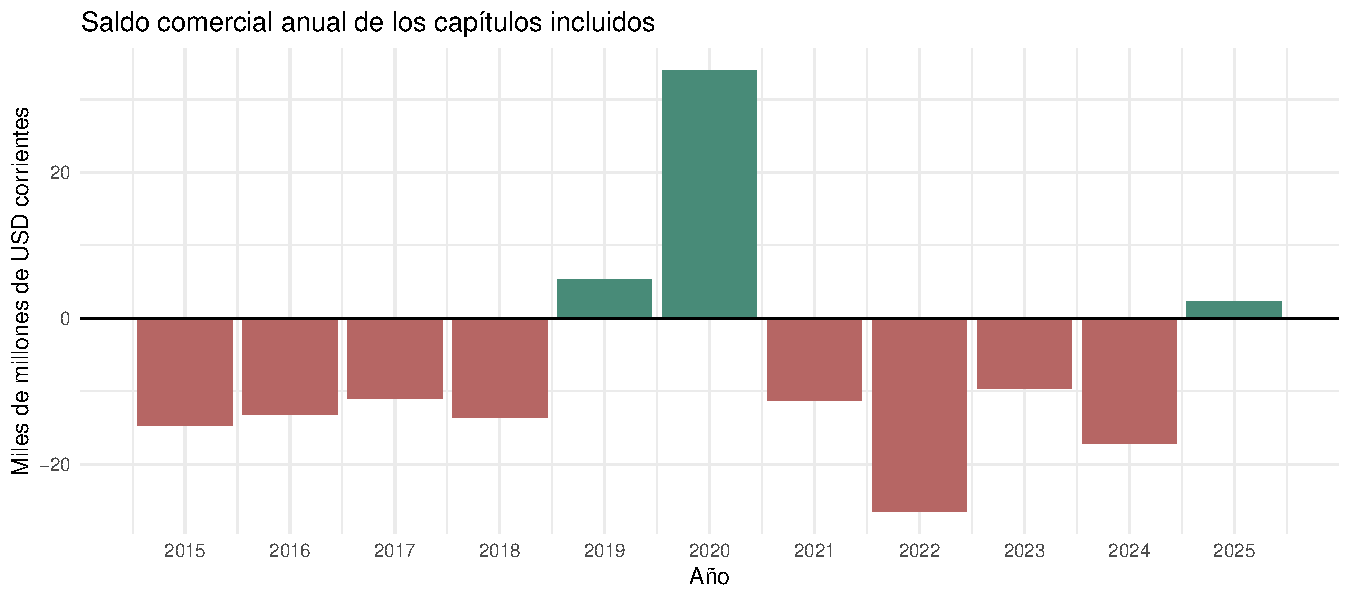
\includegraphics{Proyecto_9_EDA_files/Proyecto_9_EDA_files/figure-latex/saldo-adicional-1.pdf}
Las barras verdes indican superávit y las rojas, déficit. El cambio más
visible es de 2020 a 2021: el saldo pasa de un superávit cercano a 34
mil millones de USD a un déficit cercano a 11 mil millones.

\begin{longtable}[]{@{}rlrrr@{}}
\toprule\noalign{}
año & flow\_code & hhi\_ponderado & top1\_ponderado & capitulos \\
\midrule\noalign{}
\endhead
\bottomrule\noalign{}
\endlastfoot
2015 & M & 0.326 & 0.497 & 97 \\
2015 & X & 0.689 & 0.816 & 97 \\
2016 & M & 0.321 & 0.494 & 97 \\
2016 & X & 0.690 & 0.815 & 97 \\
2017 & M & 0.321 & 0.496 & 97 \\
2017 & X & 0.671 & 0.805 & 97 \\
2018 & M & 0.329 & 0.501 & 97 \\
2018 & X & 0.661 & 0.798 & 97 \\
2019 & M & 0.315 & 0.486 & 97 \\
2019 & X & 0.679 & 0.809 & 97 \\
2020 & M & 0.309 & 0.476 & 97 \\
2020 & X & 0.693 & 0.819 & 97 \\
2021 & M & 0.319 & 0.482 & 97 \\
2021 & X & 0.688 & 0.812 & 97 \\
2022 & M & 0.320 & 0.482 & 97 \\
2022 & X & 0.693 & 0.818 & 97 \\
2023 & M & 0.298 & 0.469 & 97 \\
2023 & X & 0.709 & 0.829 & 97 \\
2024 & M & 0.288 & 0.451 & 97 \\
2024 & X & 0.719 & 0.833 & 97 \\
2025 & M & 0.271 & 0.418 & 97 \\
2025 & X & 0.719 & 0.834 & 97 \\
\end{longtable}

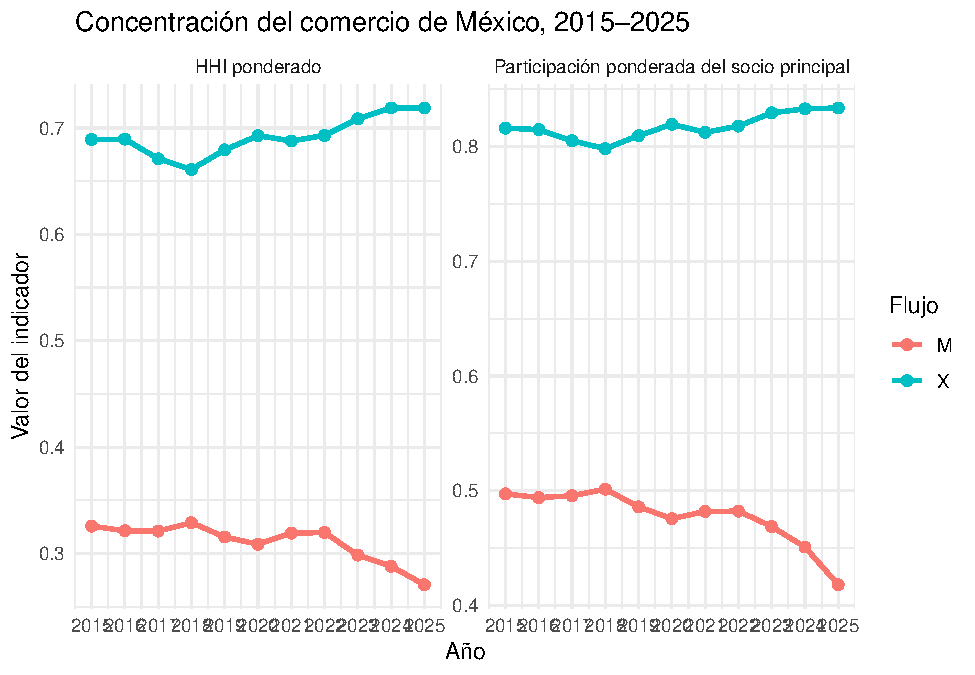
\includegraphics{Proyecto_9_EDA_files/Proyecto_9_EDA_files/figure-latex/concentracion_periodo_completo-1.pdf}

\begin{longtable}[]{@{}
  >{\raggedright\arraybackslash}p{(\columnwidth - 22\tabcolsep) * \real{0.0273}}
  >{\raggedright\arraybackslash}p{(\columnwidth - 22\tabcolsep) * \real{0.0109}}
  >{\raggedright\arraybackslash}p{(\columnwidth - 22\tabcolsep) * \real{0.5765}}
  >{\raggedleft\arraybackslash}p{(\columnwidth - 22\tabcolsep) * \real{0.0464}}
  >{\raggedleft\arraybackslash}p{(\columnwidth - 22\tabcolsep) * \real{0.0246}}
  >{\raggedleft\arraybackslash}p{(\columnwidth - 22\tabcolsep) * \real{0.0246}}
  >{\raggedleft\arraybackslash}p{(\columnwidth - 22\tabcolsep) * \real{0.0301}}
  >{\raggedleft\arraybackslash}p{(\columnwidth - 22\tabcolsep) * \real{0.0273}}
  >{\raggedleft\arraybackslash}p{(\columnwidth - 22\tabcolsep) * \real{0.0273}}
  >{\raggedleft\arraybackslash}p{(\columnwidth - 22\tabcolsep) * \real{0.0410}}
  >{\raggedright\arraybackslash}p{(\columnwidth - 22\tabcolsep) * \real{0.0574}}
  >{\raggedright\arraybackslash}p{(\columnwidth - 22\tabcolsep) * \real{0.1066}}@{}}
\toprule\noalign{}
\begin{minipage}[b]{\linewidth}\raggedright
flow\_code
\end{minipage} & \begin{minipage}[b]{\linewidth}\raggedright
hs2
\end{minipage} & \begin{minipage}[b]{\linewidth}\raggedright
capitulo
\end{minipage} & \begin{minipage}[b]{\linewidth}\raggedleft
valor\_2025\_mmusd
\end{minipage} & \begin{minipage}[b]{\linewidth}\raggedleft
hhi\_2015
\end{minipage} & \begin{minipage}[b]{\linewidth}\raggedleft
hhi\_2025
\end{minipage} & \begin{minipage}[b]{\linewidth}\raggedleft
cambio\_hhi
\end{minipage} & \begin{minipage}[b]{\linewidth}\raggedleft
top1\_2015
\end{minipage} & \begin{minipage}[b]{\linewidth}\raggedleft
top1\_2025
\end{minipage} & \begin{minipage}[b]{\linewidth}\raggedleft
cambio\_top1\_pp
\end{minipage} & \begin{minipage}[b]{\linewidth}\raggedright
socio\_principal\_2015
\end{minipage} & \begin{minipage}[b]{\linewidth}\raggedright
socio\_principal\_2025
\end{minipage} \\
\midrule\noalign{}
\endhead
\bottomrule\noalign{}
\endlastfoot
M & 84 & Machinery and mechanical appliances, boilers, nuclear reactors;
parts thereof & 144.475 & 0.223 & 0.155 & -0.068 & 0.397 & 0.245 &
-15.134 & USA & USA \\
M & 85 & Electrical machinery and equipment and parts thereof; sound
recorders and reproducers; television image and sound recorders and
reproducers, parts and accessories of such articles & 139.747 & 0.204 &
0.163 & -0.042 & 0.338 & 0.322 & -1.593 & China & China \\
M & 87 & Vehicles; other than railway or tramway rolling stock, and
parts and accessories thereof & 62.733 & 0.305 & 0.225 & -0.080 & 0.531
& 0.388 & -14.297 & USA & USA \\
M & 27 & Mineral fuels, mineral oils and products of their distillation;
bituminous substances; mineral waxes & 36.996 & 0.715 & 0.870 & 0.156 &
0.842 & 0.933 & 9.113 & USA & USA \\
M & 39 & Plastics and articles thereof & 30.703 & 0.490 & 0.396 & -0.093
& 0.692 & 0.609 & -8.300 & USA & USA \\
M & 99 & Commodities not specified according to kind & 28.291 & 0.195 &
0.230 & 0.036 & 0.368 & 0.375 & 0.712 & USA & USA \\
M & 90 & Optical, photographic, cinematographic, measuring, checking,
medical or surgical instruments and apparatus; parts and accessories &
18.480 & 0.202 & 0.228 & 0.026 & 0.368 & 0.439 & 7.092 & USA & USA \\
M & 72 & Iron and steel & 16.363 & 0.237 & 0.197 & -0.040 & 0.442 &
0.387 & -5.479 & USA & USA \\
M & 76 & Aluminium and articles thereof & 10.571 & 0.342 & 0.201 &
-0.141 & 0.562 & 0.328 & -23.417 & USA & USA \\
M & 73 & Iron or steel articles & 10.423 & 0.302 & 0.268 & -0.035 &
0.522 & 0.471 & -5.150 & USA & USA \\
X & 84 & Machinery and mechanical appliances, boilers, nuclear reactors;
parts thereof & 163.960 & 0.753 & 0.803 & 0.050 & 0.867 & 0.896 & 2.839
& USA & USA \\
X & 87 & Vehicles; other than railway or tramway rolling stock, and
parts and accessories thereof & 152.137 & 0.704 & 0.710 & 0.006 & 0.837
& 0.839 & 0.157 & USA & USA \\
X & 85 & Electrical machinery and equipment and parts thereof; sound
recorders and reproducers; television image and sound recorders and
reproducers, parts and accessories of such articles & 113.013 & 0.781 &
0.766 & -0.014 & 0.883 & 0.875 & -0.795 & USA & USA \\
X & 90 & Optical, photographic, cinematographic, measuring, checking,
medical or surgical instruments and apparatus; parts and accessories &
32.715 & 0.829 & 0.840 & 0.011 & 0.910 & 0.916 & 0.592 & USA & USA \\
X & 27 & Mineral fuels, mineral oils and products of their distillation;
bituminous substances; mineral waxes & 20.575 & 0.384 & 0.286 & -0.098 &
0.605 & 0.431 & -17.382 & USA & North America and Central America,
nes \\
X & 26 & Ores, slag and ash & 12.888 & 0.190 & 0.276 & 0.086 & 0.287 &
0.456 & 16.902 & China & China \\
X & 94 & Furniture; bedding, mattresses, mattress supports, cushions and
similar stuffed furnishings; lamps and lighting fittings, n.e.c.;
illuminated signs, illuminated name-plates and the like; prefabricated
buildings & 12.581 & 0.874 & 0.868 & -0.006 & 0.934 & 0.930 & -0.384 &
USA & USA \\
X & 39 & Plastics and articles thereof & 12.252 & 0.562 & 0.680 & 0.118
& 0.748 & 0.824 & 7.602 & USA & USA \\
X & 22 & Beverages, spirits and vinegar & 11.842 & 0.607 & 0.758 & 0.151
& 0.777 & 0.870 & 9.320 & USA & USA \\
X & 71 & Natural, cultured pearls; precious, semi-precious stones;
precious metals, metals clad with precious metal, and articles thereof;
imitation jewellery; coin & 11.160 & 0.605 & 0.477 & -0.128 & 0.764 &
0.663 & -10.073 & USA & USA \\
\end{longtable}

Con las etiquetas originales, las importaciones muestran una menor
concentración promedio durante 2015--2025 y las exportaciones permanecen
más concentradas. Esta lectura descriptiva se contrasta más adelante con
indicadores calculados solo entre socios geográficos identificados, dado
el aumento de etiquetas no específicas en 2025.

\subsubsection{2. Del tamaño del capítulo a su
concentración}\label{del-tamauxf1o-del-capuxedtulo-a-su-concentraciuxf3n}

\texttt{participacion} ya indica el peso de cada capítulo dentro de las
importaciones del mismo año. Se compara con el HHI: un capítulo muy
concentrado pero pequeño cuenta una historia diferente a uno que combina
alto valor y concentración. Para evitar basar una conclusión en un solo
año, se contrastan promedios de 2015--2017 y 2023--2025.

\begin{Shaded}
\begin{Highlighting}[]
\NormalTok{perfil\_hs2 }\OtherTok{\textless{}{-}}\NormalTok{ indicadores }\SpecialCharTok{\%\textgreater{}\%}
  \FunctionTok{filter}\NormalTok{(flow\_code }\SpecialCharTok{==} \StringTok{"M"}\NormalTok{) }\SpecialCharTok{\%\textgreater{}\%}
  \FunctionTok{group\_by}\NormalTok{(hs2) }\SpecialCharTok{\%\textgreater{}\%}
  \FunctionTok{summarise}\NormalTok{(}
    \AttributeTok{capitulo =} \FunctionTok{first}\NormalTok{(capitulo),}
\NormalTok{    años}\AttributeTok{\_observados =} \FunctionTok{n\_distinct}\NormalTok{(año),}
\NormalTok{    años}\AttributeTok{\_inicio =} \FunctionTok{sum}\NormalTok{(año }\SpecialCharTok{\%in\%} \DecValTok{2015}\SpecialCharTok{:}\DecValTok{2017}\NormalTok{),}
\NormalTok{    años}\AttributeTok{\_fin =} \FunctionTok{sum}\NormalTok{(año }\SpecialCharTok{\%in\%} \DecValTok{2023}\SpecialCharTok{:}\DecValTok{2025}\NormalTok{),}
    \AttributeTok{hhi\_medio =} \FunctionTok{mean}\NormalTok{(hhi),}
    \AttributeTok{hhi\_inicio =} \FunctionTok{mean}\NormalTok{(hhi[año }\SpecialCharTok{\%in\%} \DecValTok{2015}\SpecialCharTok{:}\DecValTok{2017}\NormalTok{]),}
    \AttributeTok{hhi\_fin =} \FunctionTok{mean}\NormalTok{(hhi[año }\SpecialCharTok{\%in\%} \DecValTok{2023}\SpecialCharTok{:}\DecValTok{2025}\NormalTok{]),}
    \AttributeTok{participacion\_media =} \FunctionTok{mean}\NormalTok{(participacion),}
    \AttributeTok{participacion\_inicio =} \FunctionTok{mean}\NormalTok{(participacion[año }\SpecialCharTok{\%in\%} \DecValTok{2015}\SpecialCharTok{:}\DecValTok{2017}\NormalTok{]),}
    \AttributeTok{participacion\_fin =} \FunctionTok{mean}\NormalTok{(participacion[año }\SpecialCharTok{\%in\%} \DecValTok{2023}\SpecialCharTok{:}\DecValTok{2025}\NormalTok{]),}
    \AttributeTok{.groups =} \StringTok{"drop"}
\NormalTok{  ) }\SpecialCharTok{\%\textgreater{}\%}
  \FunctionTok{filter}\NormalTok{(años\_observados }\SpecialCharTok{\textgreater{}=} \DecValTok{8}\NormalTok{, años\_inicio }\SpecialCharTok{==} \DecValTok{3}\NormalTok{, años\_fin }\SpecialCharTok{==} \DecValTok{3}\NormalTok{) }\SpecialCharTok{\%\textgreater{}\%}
  \FunctionTok{mutate}\NormalTok{(}\AttributeTok{cambio\_hhi =}\NormalTok{ hhi\_fin }\SpecialCharTok{{-}}\NormalTok{ hhi\_inicio,}
         \AttributeTok{cambio\_peso\_pp =} \DecValTok{100} \SpecialCharTok{*}\NormalTok{ (participacion\_fin }\SpecialCharTok{{-}}\NormalTok{ participacion\_inicio))}

\NormalTok{knitr}\SpecialCharTok{::}\FunctionTok{kable}\NormalTok{(perfil\_hs2 }\SpecialCharTok{\%\textgreater{}\%} \FunctionTok{arrange}\NormalTok{(}\FunctionTok{desc}\NormalTok{(cambio\_hhi)) }\SpecialCharTok{\%\textgreater{}\%}
               \FunctionTok{select}\NormalTok{(hs2, capitulo, hhi\_inicio, hhi\_fin,}
\NormalTok{                      cambio\_hhi, participacion\_fin) }\SpecialCharTok{\%\textgreater{}\%} \FunctionTok{head}\NormalTok{(}\DecValTok{10}\NormalTok{),}
             \AttributeTok{digits =} \DecValTok{3}\NormalTok{, }\AttributeTok{caption =} \StringTok{"Capítulos con mayor aumento del HHI importador"}\NormalTok{)}
\end{Highlighting}
\end{Shaded}

\begin{longtable}[]{@{}
  >{\raggedright\arraybackslash}p{(\columnwidth - 10\tabcolsep) * \real{0.0242}}
  >{\raggedright\arraybackslash}p{(\columnwidth - 10\tabcolsep) * \real{0.6848}}
  >{\raggedleft\arraybackslash}p{(\columnwidth - 10\tabcolsep) * \real{0.0667}}
  >{\raggedleft\arraybackslash}p{(\columnwidth - 10\tabcolsep) * \real{0.0485}}
  >{\raggedleft\arraybackslash}p{(\columnwidth - 10\tabcolsep) * \real{0.0667}}
  >{\raggedleft\arraybackslash}p{(\columnwidth - 10\tabcolsep) * \real{0.1091}}@{}}
\caption{Capítulos con mayor aumento del HHI importador}\tabularnewline
\toprule\noalign{}
\begin{minipage}[b]{\linewidth}\raggedright
hs2
\end{minipage} & \begin{minipage}[b]{\linewidth}\raggedright
capitulo
\end{minipage} & \begin{minipage}[b]{\linewidth}\raggedleft
hhi\_inicio
\end{minipage} & \begin{minipage}[b]{\linewidth}\raggedleft
hhi\_fin
\end{minipage} & \begin{minipage}[b]{\linewidth}\raggedleft
cambio\_hhi
\end{minipage} & \begin{minipage}[b]{\linewidth}\raggedleft
participacion\_fin
\end{minipage} \\
\midrule\noalign{}
\endfirsthead
\toprule\noalign{}
\begin{minipage}[b]{\linewidth}\raggedright
hs2
\end{minipage} & \begin{minipage}[b]{\linewidth}\raggedright
capitulo
\end{minipage} & \begin{minipage}[b]{\linewidth}\raggedleft
hhi\_inicio
\end{minipage} & \begin{minipage}[b]{\linewidth}\raggedleft
hhi\_fin
\end{minipage} & \begin{minipage}[b]{\linewidth}\raggedleft
cambio\_hhi
\end{minipage} & \begin{minipage}[b]{\linewidth}\raggedleft
participacion\_fin
\end{minipage} \\
\midrule\noalign{}
\endhead
\bottomrule\noalign{}
\endlastfoot
14 & Vegetable plaiting materials; vegetable products not elsewhere
specified or included & 0.170 & 0.492 & 0.323 & 0.000 \\
26 & Ores, slag and ash & 0.179 & 0.415 & 0.236 & 0.003 \\
67 & Feathers and down, prepared; and articles made of feather or of
down; artificial flowers; articles of human hair & 0.668 & 0.892 & 0.224
& 0.000 \\
91 & Clocks and watches and parts thereof & 0.359 & 0.541 & 0.181 &
0.001 \\
50 & Silk & 0.256 & 0.416 & 0.160 & 0.000 \\
24 & Tobacco and manufactured tobacco substitutes & 0.360 & 0.520 &
0.159 & 0.000 \\
93 & Arms and ammunition; parts and accessories thereof & 0.212 & 0.361
& 0.149 & 0.000 \\
89 & Ships, boats and floating structures & 0.342 & 0.458 & 0.116 &
0.000 \\
75 & Nickel and articles thereof & 0.340 & 0.437 & 0.097 & 0.001 \\
27 & Mineral fuels, mineral oils and products of their distillation;
bituminous substances; mineral waxes & 0.743 & 0.838 & 0.095 & 0.068 \\
\end{longtable}

\begin{Shaded}
\begin{Highlighting}[]
\NormalTok{knitr}\SpecialCharTok{::}\FunctionTok{kable}\NormalTok{(perfil\_hs2 }\SpecialCharTok{\%\textgreater{}\%} \FunctionTok{arrange}\NormalTok{(cambio\_hhi) }\SpecialCharTok{\%\textgreater{}\%}
               \FunctionTok{select}\NormalTok{(hs2, capitulo, hhi\_inicio, hhi\_fin,}
\NormalTok{                      cambio\_hhi, participacion\_fin) }\SpecialCharTok{\%\textgreater{}\%} \FunctionTok{head}\NormalTok{(}\DecValTok{10}\NormalTok{),}
             \AttributeTok{digits =} \DecValTok{3}\NormalTok{, }\AttributeTok{caption =} \StringTok{"Capítulos con mayor reducción del HHI importador"}\NormalTok{)}
\end{Highlighting}
\end{Shaded}

\begin{longtable}[]{@{}
  >{\raggedright\arraybackslash}p{(\columnwidth - 10\tabcolsep) * \real{0.0192}}
  >{\raggedright\arraybackslash}p{(\columnwidth - 10\tabcolsep) * \real{0.7500}}
  >{\raggedleft\arraybackslash}p{(\columnwidth - 10\tabcolsep) * \real{0.0529}}
  >{\raggedleft\arraybackslash}p{(\columnwidth - 10\tabcolsep) * \real{0.0385}}
  >{\raggedleft\arraybackslash}p{(\columnwidth - 10\tabcolsep) * \real{0.0529}}
  >{\raggedleft\arraybackslash}p{(\columnwidth - 10\tabcolsep) * \real{0.0865}}@{}}
\caption{Capítulos con mayor reducción del HHI
importador}\tabularnewline
\toprule\noalign{}
\begin{minipage}[b]{\linewidth}\raggedright
hs2
\end{minipage} & \begin{minipage}[b]{\linewidth}\raggedright
capitulo
\end{minipage} & \begin{minipage}[b]{\linewidth}\raggedleft
hhi\_inicio
\end{minipage} & \begin{minipage}[b]{\linewidth}\raggedleft
hhi\_fin
\end{minipage} & \begin{minipage}[b]{\linewidth}\raggedleft
cambio\_hhi
\end{minipage} & \begin{minipage}[b]{\linewidth}\raggedleft
participacion\_fin
\end{minipage} \\
\midrule\noalign{}
\endfirsthead
\toprule\noalign{}
\begin{minipage}[b]{\linewidth}\raggedright
hs2
\end{minipage} & \begin{minipage}[b]{\linewidth}\raggedright
capitulo
\end{minipage} & \begin{minipage}[b]{\linewidth}\raggedleft
hhi\_inicio
\end{minipage} & \begin{minipage}[b]{\linewidth}\raggedleft
hhi\_fin
\end{minipage} & \begin{minipage}[b]{\linewidth}\raggedleft
cambio\_hhi
\end{minipage} & \begin{minipage}[b]{\linewidth}\raggedleft
participacion\_fin
\end{minipage} \\
\midrule\noalign{}
\endhead
\bottomrule\noalign{}
\endlastfoot
57 & Carpets and other textile floor coverings & 0.481 & 0.243 & -0.238
& 0.000 \\
56 & Wadding, felt and nonwovens, special yarns; twine, cordage, ropes
and cables and articles thereof & 0.564 & 0.330 & -0.235 & 0.002 \\
59 & Textile fabrics; impregnated, coated, covered or laminated; textile
articles of a kind suitable for industrial use & 0.562 & 0.341 & -0.221
& 0.002 \\
79 & Zinc and articles thereof & 0.453 & 0.242 & -0.211 & 0.000 \\
17 & Sugars and sugar confectionery & 0.766 & 0.572 & -0.194 & 0.003 \\
05 & Animal originated products; not elsewhere specified or included &
0.761 & 0.577 & -0.184 & 0.001 \\
95 & Toys, games and sports requisites; parts and accessories thereof &
0.549 & 0.368 & -0.182 & 0.005 \\
11 & Products of the milling industry; malt, starches, inulin, wheat
gluten & 0.577 & 0.398 & -0.179 & 0.001 \\
37 & Photographic or cinematographic goods & 0.428 & 0.251 & -0.177 &
0.000 \\
71 & Natural, cultured pearls; precious, semi-precious stones; precious
metals, metals clad with precious metal, and articles thereof; imitation
jewellery; coin & 0.322 & 0.160 & -0.163 & 0.003 \\
\end{longtable}

\begin{Shaded}
\begin{Highlighting}[]
\NormalTok{knitr}\SpecialCharTok{::}\FunctionTok{kable}\NormalTok{(perfil\_hs2 }\SpecialCharTok{\%\textgreater{}\%} \FunctionTok{arrange}\NormalTok{(}\FunctionTok{desc}\NormalTok{(}\FunctionTok{abs}\NormalTok{(cambio\_peso\_pp))) }\SpecialCharTok{\%\textgreater{}\%}
               \FunctionTok{select}\NormalTok{(hs2, capitulo, participacion\_inicio,}
\NormalTok{                      participacion\_fin, cambio\_peso\_pp) }\SpecialCharTok{\%\textgreater{}\%} \FunctionTok{head}\NormalTok{(}\DecValTok{10}\NormalTok{),}
             \AttributeTok{digits =} \DecValTok{3}\NormalTok{,}
             \AttributeTok{caption =} \StringTok{"Mayores cambios absolutos de peso (puntos porcentuales)"}\NormalTok{)}
\end{Highlighting}
\end{Shaded}

\begin{longtable}[]{@{}
  >{\raggedright\arraybackslash}p{(\columnwidth - 8\tabcolsep) * \real{0.0168}}
  >{\raggedright\arraybackslash}p{(\columnwidth - 8\tabcolsep) * \real{0.7563}}
  >{\raggedleft\arraybackslash}p{(\columnwidth - 8\tabcolsep) * \real{0.0882}}
  >{\raggedleft\arraybackslash}p{(\columnwidth - 8\tabcolsep) * \real{0.0756}}
  >{\raggedleft\arraybackslash}p{(\columnwidth - 8\tabcolsep) * \real{0.0630}}@{}}
\caption{Mayores cambios absolutos de peso (puntos
porcentuales)}\tabularnewline
\toprule\noalign{}
\begin{minipage}[b]{\linewidth}\raggedright
hs2
\end{minipage} & \begin{minipage}[b]{\linewidth}\raggedright
capitulo
\end{minipage} & \begin{minipage}[b]{\linewidth}\raggedleft
participacion\_inicio
\end{minipage} & \begin{minipage}[b]{\linewidth}\raggedleft
participacion\_fin
\end{minipage} & \begin{minipage}[b]{\linewidth}\raggedleft
cambio\_peso\_pp
\end{minipage} \\
\midrule\noalign{}
\endfirsthead
\toprule\noalign{}
\begin{minipage}[b]{\linewidth}\raggedright
hs2
\end{minipage} & \begin{minipage}[b]{\linewidth}\raggedright
capitulo
\end{minipage} & \begin{minipage}[b]{\linewidth}\raggedleft
participacion\_inicio
\end{minipage} & \begin{minipage}[b]{\linewidth}\raggedleft
participacion\_fin
\end{minipage} & \begin{minipage}[b]{\linewidth}\raggedleft
cambio\_peso\_pp
\end{minipage} \\
\midrule\noalign{}
\endhead
\bottomrule\noalign{}
\endlastfoot
99 & Commodities not specified according to kind & 0.033 & 0.045 &
1.235 \\
84 & Nuclear reactors, boilers, machinery and mechanical appliances;
parts thereof & 0.171 & 0.183 & 1.148 \\
90 & Optical, photographic, cinematographic, measuring, checking,
medical or surgical instruments and apparatus; parts and accessories &
0.037 & 0.028 & -0.905 \\
72 & Iron and steel & 0.023 & 0.031 & 0.723 \\
39 & Plastics and articles thereof & 0.056 & 0.049 & -0.712 \\
85 & Electrical machinery and equipment and parts thereof; sound
recorders and reproducers; television image and sound recorders and
reproducers, parts and accessories of such articles & 0.213 & 0.206 &
-0.697 \\
73 & Iron or steel articles & 0.023 & 0.018 & -0.470 \\
27 & Mineral fuels, mineral oils and products of their distillation;
bituminous substances; mineral waxes & 0.072 & 0.068 & -0.449 \\
29 & Organic chemicals & 0.020 & 0.017 & -0.333 \\
87 & Vehicles; other than railway or tramway rolling stock, and parts
and accessories thereof & 0.097 & 0.100 & 0.301 \\
\end{longtable}

\begin{itemize}
\item
  HS84, maquinaria mecánica, pasó de representar aproximadamente 17.1 \%
  a 18.3 \% de las importaciones: ganó 1.148 puntos porcentuales. Este
  dato confirma que HS84 es importante y debe aparecer cuando corrijas
  la tabla comparativa de HHI.
\item
  HS85, equipo eléctrico, perdió 0.697 puntos porcentuales, pero siguió
  siendo el capítulo de mayor peso entre los mostrados: 20.6 \% en el
  periodo final. Juntos, HS84 y HS85 representan aproximadamente 38.9
  \%.
\end{itemize}

Además del HHI, esta tabla muestra si cambió el país que tenía la cuota
más alta en cada capítulo. El cambio de líder no prueba por sí solo que
todos los demás proveedores hayan cambiado.

\begin{Shaded}
\begin{Highlighting}[]
\NormalTok{cambio\_lider }\OtherTok{\textless{}{-}}\NormalTok{ indicadores }\SpecialCharTok{\%\textgreater{}\%}
  \FunctionTok{filter}\NormalTok{(flow\_code }\SpecialCharTok{==} \StringTok{"M"}\NormalTok{, año }\SpecialCharTok{\%in\%} \FunctionTok{c}\NormalTok{(}\DecValTok{2015}\NormalTok{, }\DecValTok{2025}\NormalTok{)) }\SpecialCharTok{\%\textgreater{}\%}
  \FunctionTok{select}\NormalTok{(año, hs2, socio\_principal, top1, valor\_usd) }\SpecialCharTok{\%\textgreater{}\%}
  \FunctionTok{pivot\_wider}\NormalTok{(}\AttributeTok{names\_from =}\NormalTok{ año,}
              \AttributeTok{values\_from =} \FunctionTok{c}\NormalTok{(socio\_principal, top1, valor\_usd)) }\SpecialCharTok{\%\textgreater{}\%}
  \FunctionTok{filter}\NormalTok{(}\SpecialCharTok{!}\FunctionTok{is.na}\NormalTok{(socio\_principal\_2015), }\SpecialCharTok{!}\FunctionTok{is.na}\NormalTok{(socio\_principal\_2025)) }\SpecialCharTok{\%\textgreater{}\%}
  \FunctionTok{mutate}\NormalTok{(}\AttributeTok{cambio\_de\_lider =}\NormalTok{ socio\_principal\_2015 }\SpecialCharTok{!=}\NormalTok{ socio\_principal\_2025) }\SpecialCharTok{\%\textgreater{}\%}
  \FunctionTok{arrange}\NormalTok{(}\FunctionTok{desc}\NormalTok{(valor\_usd\_2025))}
\NormalTok{knitr}\SpecialCharTok{::}\FunctionTok{kable}\NormalTok{(cambio\_lider }\SpecialCharTok{\%\textgreater{}\%} \FunctionTok{head}\NormalTok{(}\DecValTok{15}\NormalTok{), }\AttributeTok{digits =} \DecValTok{3}\NormalTok{,}
             \AttributeTok{caption =} \StringTok{"Proveedor principal en 2015 y 2025 para los capítulos de mayor valor en 2025"}\NormalTok{)}
\end{Highlighting}
\end{Shaded}

\begin{longtable}[]{@{}
  >{\raggedright\arraybackslash}p{(\columnwidth - 14\tabcolsep) * \real{0.0357}}
  >{\raggedright\arraybackslash}p{(\columnwidth - 14\tabcolsep) * \real{0.1875}}
  >{\raggedright\arraybackslash}p{(\columnwidth - 14\tabcolsep) * \real{0.1875}}
  >{\raggedleft\arraybackslash}p{(\columnwidth - 14\tabcolsep) * \real{0.0893}}
  >{\raggedleft\arraybackslash}p{(\columnwidth - 14\tabcolsep) * \real{0.0893}}
  >{\raggedleft\arraybackslash}p{(\columnwidth - 14\tabcolsep) * \real{0.1339}}
  >{\raggedleft\arraybackslash}p{(\columnwidth - 14\tabcolsep) * \real{0.1339}}
  >{\raggedright\arraybackslash}p{(\columnwidth - 14\tabcolsep) * \real{0.1429}}@{}}
\caption{Proveedor principal en 2015 y 2025 para los capítulos de mayor
valor en 2025}\tabularnewline
\toprule\noalign{}
\begin{minipage}[b]{\linewidth}\raggedright
hs2
\end{minipage} & \begin{minipage}[b]{\linewidth}\raggedright
socio\_principal\_2015
\end{minipage} & \begin{minipage}[b]{\linewidth}\raggedright
socio\_principal\_2025
\end{minipage} & \begin{minipage}[b]{\linewidth}\raggedleft
top1\_2015
\end{minipage} & \begin{minipage}[b]{\linewidth}\raggedleft
top1\_2025
\end{minipage} & \begin{minipage}[b]{\linewidth}\raggedleft
valor\_usd\_2015
\end{minipage} & \begin{minipage}[b]{\linewidth}\raggedleft
valor\_usd\_2025
\end{minipage} & \begin{minipage}[b]{\linewidth}\raggedright
cambio\_de\_lider
\end{minipage} \\
\midrule\noalign{}
\endfirsthead
\toprule\noalign{}
\begin{minipage}[b]{\linewidth}\raggedright
hs2
\end{minipage} & \begin{minipage}[b]{\linewidth}\raggedright
socio\_principal\_2015
\end{minipage} & \begin{minipage}[b]{\linewidth}\raggedright
socio\_principal\_2025
\end{minipage} & \begin{minipage}[b]{\linewidth}\raggedleft
top1\_2015
\end{minipage} & \begin{minipage}[b]{\linewidth}\raggedleft
top1\_2025
\end{minipage} & \begin{minipage}[b]{\linewidth}\raggedleft
valor\_usd\_2015
\end{minipage} & \begin{minipage}[b]{\linewidth}\raggedleft
valor\_usd\_2025
\end{minipage} & \begin{minipage}[b]{\linewidth}\raggedright
cambio\_de\_lider
\end{minipage} \\
\midrule\noalign{}
\endhead
\bottomrule\noalign{}
\endlastfoot
84 & USA & USA & 0.397 & 0.245 & 67685896944 & 144474585274 & FALSE \\
85 & China & China & 0.338 & 0.322 & 85413675736 & 139747265525 &
FALSE \\
87 & USA & USA & 0.531 & 0.388 & 37266625012 & 62732602616 & FALSE \\
27 & USA & USA & 0.842 & 0.933 & 26455515248 & 36996200959 & FALSE \\
39 & USA & USA & 0.692 & 0.609 & 22308496453 & 30703144257 & FALSE \\
99 & USA & USA & 0.368 & 0.375 & 11703403716 & 28290698387 & FALSE \\
90 & USA & USA & 0.368 & 0.439 & 14989763051 & 18479894427 & FALSE \\
72 & USA & USA & 0.442 & 0.387 & 9406974542 & 16362694975 & FALSE \\
76 & USA & USA & 0.562 & 0.328 & 5481953514 & 10571345489 & FALSE \\
73 & USA & USA & 0.522 & 0.471 & 9386558048 & 10422586532 & FALSE \\
29 & USA & USA & 0.601 & 0.577 & 8075484409 & 10131290401 & FALSE \\
30 & USA & USA & 0.296 & 0.230 & 4804125675 & 10078507828 & FALSE \\
02 & USA & USA & 0.825 & 0.659 & 3820538832 & 9116591063 & FALSE \\
40 & USA & USA & 0.473 & 0.395 & 6565063892 & 8461094314 & FALSE \\
10 & USA & USA & 0.868 & 0.896 & 4005357279 & 8179909620 & FALSE \\
\end{longtable}

Entre los capítulos de mayor valor importado en 2025, no se observó un
cambio de proveedor principal al comparar 2015 con 2025. Sin embargo, sí
cambió cuánto valor concentraba ese proveedor. La cuota del líder
disminuyó notablemente en maquinaria mecánica, vehículos y aluminio,
mientras que aumentó en combustibles. Por ello, la permanencia de un
país en primer lugar no implica que la concentración comercial
permanezca constante.

\begin{Shaded}
\begin{Highlighting}[]
\NormalTok{vista\_2025 }\OtherTok{\textless{}{-}}\NormalTok{ indicadores }\SpecialCharTok{\%\textgreater{}\%} \FunctionTok{filter}\NormalTok{(año }\SpecialCharTok{==} \DecValTok{2025}\NormalTok{, flow\_code }\SpecialCharTok{==} \StringTok{"M"}\NormalTok{)}
\NormalTok{etiquetas\_2025 }\OtherTok{\textless{}{-}}\NormalTok{ vista\_2025 }\SpecialCharTok{\%\textgreater{}\%} \FunctionTok{slice\_max}\NormalTok{(valor\_usd, }\AttributeTok{n =} \DecValTok{12}\NormalTok{)}
\FunctionTok{ggplot}\NormalTok{(vista\_2025, }\FunctionTok{aes}\NormalTok{(participacion, hhi, }\AttributeTok{size =}\NormalTok{ valor\_usd }\SpecialCharTok{/} \FloatTok{1e9}\NormalTok{)) }\SpecialCharTok{+}
  \FunctionTok{geom\_point}\NormalTok{(}\AttributeTok{color =} \StringTok{"\#537d9b"}\NormalTok{, }\AttributeTok{alpha =} \FloatTok{0.65}\NormalTok{) }\SpecialCharTok{+}
\NormalTok{  ggrepel}\SpecialCharTok{::}\FunctionTok{geom\_text\_repel}\NormalTok{(}\AttributeTok{data =}\NormalTok{ etiquetas\_2025, }\FunctionTok{aes}\NormalTok{(}\AttributeTok{label =}\NormalTok{ hs2),}
                           \AttributeTok{size =} \DecValTok{3}\NormalTok{, }\AttributeTok{show.legend =} \ConstantTok{FALSE}\NormalTok{) }\SpecialCharTok{+}
  \FunctionTok{scale\_x\_log10}\NormalTok{(}\AttributeTok{labels =}\NormalTok{ scales}\SpecialCharTok{::}\NormalTok{percent) }\SpecialCharTok{+}
  \FunctionTok{labs}\NormalTok{(}\AttributeTok{title =} \StringTok{"Peso económico y concentración por capítulo en 2025"}\NormalTok{,}
       \AttributeTok{subtitle =} \StringTok{"Se etiquetan los 12 capítulos de mayor valor importado"}\NormalTok{,}
       \AttributeTok{x =} \StringTok{"Porcentaje de las importaciones (escala logarítmica)"}\NormalTok{,}
       \AttributeTok{y =} \StringTok{"HHI de proveedores"}\NormalTok{, }\AttributeTok{size =} \StringTok{"Miles de millones}\SpecialCharTok{\textbackslash{}n}\StringTok{de USD"}\NormalTok{) }\SpecialCharTok{+}
  \FunctionTok{theme\_minimal}\NormalTok{()}
\end{Highlighting}
\end{Shaded}

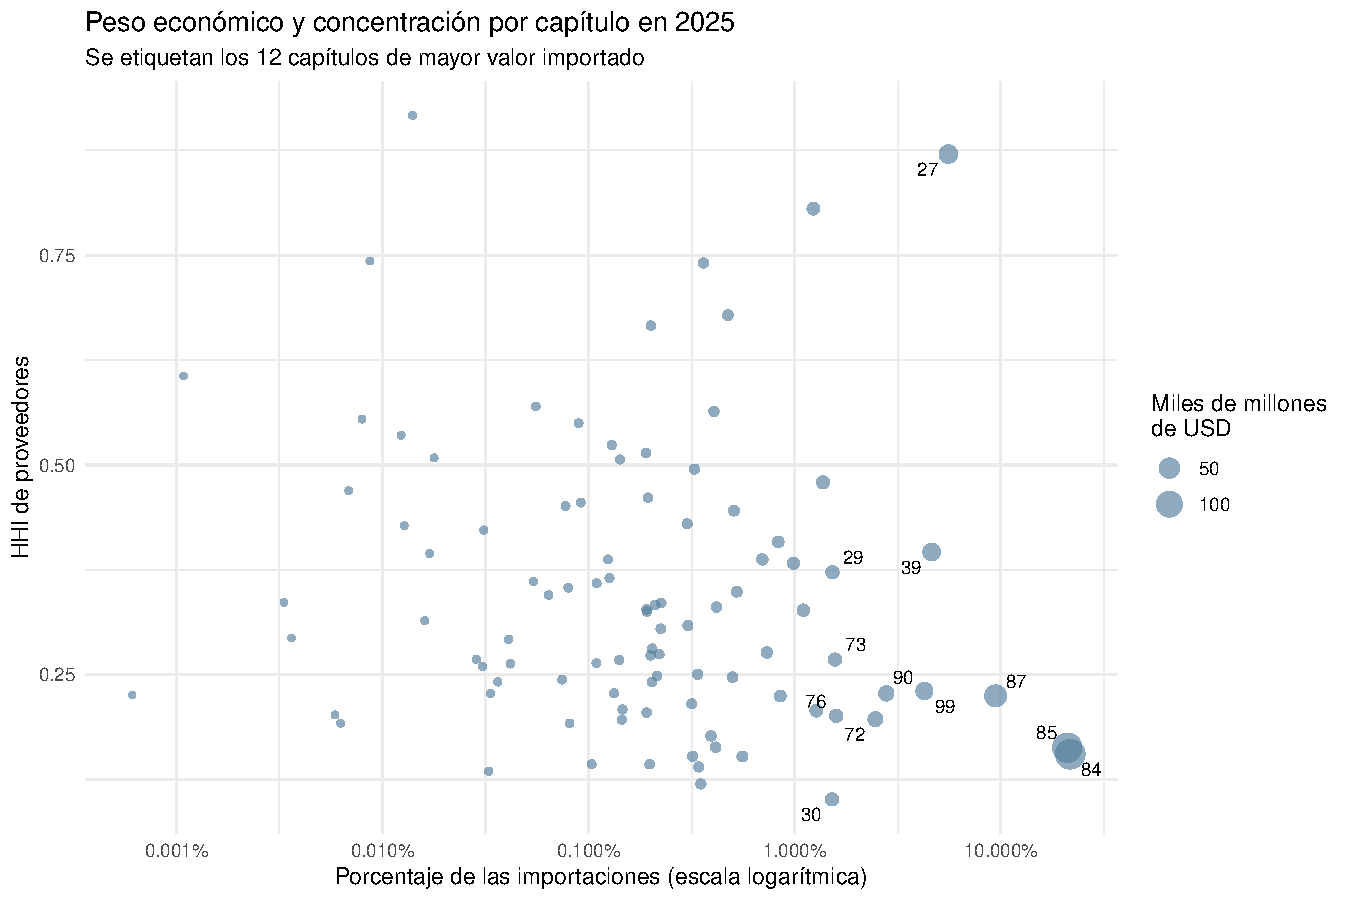
\includegraphics{Proyecto_9_EDA_files/Proyecto_9_EDA_files/figure-latex/concentracion-y-peso-1.pdf}

Arriba y a la derecha están los capítulos que combinan mayor
concentración y participación. La ubicación no demuestra riesgo de
desabasto: el HHI mide valor, no cantidades físicas ni facilidad de
cambiar de proveedor. Las variaciones nominales también pueden reflejar
precios.

En 2025, los capítulos de mayor valor importado no fueron necesariamente
los más concentrados. Maquinaria mecánica (HS84) y equipo eléctrico
(HS85) tuvieron un HHI relativamente bajo con las etiquetas originales.
Combustibles (HS27) combinó un valor importante con alta concentración.
El HHI de HS84 y HS85 se revisa más adelante porque parte de su valor
corresponde a etiquetas de socio no específicas.

\subsubsection{3. Preparación de datos para el
modelo}\label{preparaciuxf3n-de-datos-para-el-modelo}

La unidad del modelo es el \textbf{capítulo HS2 de importaciones}: cada
fila resume su comportamiento entre 2015 y 2025. Antes de agruparlos,
revisamos la cobertura temporal y las etiquetas que no identifican un
país. El capítulo HS99 se conserva en el análisis descriptivo, pero se
excluye del agrupamiento porque reúne mercancías sin una categoría de
producto especificada.

\begin{longtable}[]{@{}
  >{\raggedleft\arraybackslash}p{(\columnwidth - 6\tabcolsep) * \real{0.1622}}
  >{\raggedright\arraybackslash}p{(\columnwidth - 6\tabcolsep) * \real{0.5270}}
  >{\raggedleft\arraybackslash}p{(\columnwidth - 6\tabcolsep) * \real{0.1351}}
  >{\raggedleft\arraybackslash}p{(\columnwidth - 6\tabcolsep) * \real{0.1757}}@{}}
\caption{Etiquetas de socios no especificados en
importaciones}\tabularnewline
\toprule\noalign{}
\begin{minipage}[b]{\linewidth}\raggedleft
partnerCode
\end{minipage} & \begin{minipage}[b]{\linewidth}\raggedright
partnerDesc
\end{minipage} & \begin{minipage}[b]{\linewidth}\raggedleft
registros
\end{minipage} & \begin{minipage}[b]{\linewidth}\raggedleft
valor\_usd
\end{minipage} \\
\midrule\noalign{}
\endfirsthead
\toprule\noalign{}
\begin{minipage}[b]{\linewidth}\raggedleft
partnerCode
\end{minipage} & \begin{minipage}[b]{\linewidth}\raggedright
partnerDesc
\end{minipage} & \begin{minipage}[b]{\linewidth}\raggedleft
registros
\end{minipage} & \begin{minipage}[b]{\linewidth}\raggedleft
valor\_usd
\end{minipage} \\
\midrule\noalign{}
\endhead
\bottomrule\noalign{}
\endlastfoot
490 & Other Asia, nes & 810 & 152531765871 \\
899 & Areas, nes & 1067 & 23593381188 \\
568 & Other Europe, nes & 396 & 1161900955 \\
637 & North America and Central America, nes & 1 & 447 \\
\end{longtable}

\begin{longtable}[]{@{}rr@{}}
\caption{Cobertura temporal de los capítulos candidatos}\tabularnewline
\toprule\noalign{}
años\_observados & capitulos \\
\midrule\noalign{}
\endfirsthead
\toprule\noalign{}
años\_observados & capitulos \\
\midrule\noalign{}
\endhead
\bottomrule\noalign{}
\endlastfoot
11 & 97 \\
\end{longtable}

\begin{longtable}[]{@{}
  >{\raggedleft\arraybackslash}p{(\columnwidth - 6\tabcolsep) * \real{0.0676}}
  >{\raggedleft\arraybackslash}p{(\columnwidth - 6\tabcolsep) * \real{0.2162}}
  >{\raggedleft\arraybackslash}p{(\columnwidth - 6\tabcolsep) * \real{0.3514}}
  >{\raggedleft\arraybackslash}p{(\columnwidth - 6\tabcolsep) * \real{0.3649}}@{}}
\caption{Peso anual de las etiquetas de socio no
especificado}\tabularnewline
\toprule\noalign{}
\begin{minipage}[b]{\linewidth}\raggedleft
año
\end{minipage} & \begin{minipage}[b]{\linewidth}\raggedleft
valor\_total\_usd
\end{minipage} & \begin{minipage}[b]{\linewidth}\raggedleft
valor\_no\_especificado\_usd
\end{minipage} & \begin{minipage}[b]{\linewidth}\raggedleft
porcentaje\_no\_especificado
\end{minipage} \\
\midrule\noalign{}
\endfirsthead
\toprule\noalign{}
\begin{minipage}[b]{\linewidth}\raggedleft
año
\end{minipage} & \begin{minipage}[b]{\linewidth}\raggedleft
valor\_total\_usd
\end{minipage} & \begin{minipage}[b]{\linewidth}\raggedleft
valor\_no\_especificado\_usd
\end{minipage} & \begin{minipage}[b]{\linewidth}\raggedleft
porcentaje\_no\_especificado
\end{minipage} \\
\midrule\noalign{}
\endhead
\bottomrule\noalign{}
\endlastfoot
2015 & 395253856855 & 7364809003 & 1.86 \\
2016 & 387087412856 & 7583133426 & 1.96 \\
2017 & 420394590810 & 8317612928 & 1.98 \\
2018 & 464294259444 & 9080781982 & 1.96 \\
2019 & 455235784381 & 10305468557 & 2.26 \\
2020 & 382979895758 & 9363797580 & 2.44 \\
2021 & 505715615701 & 14825571130 & 2.93 \\
2022 & 606295621090 & 19283708309 & 3.18 \\
2023 & 605582537052 & 18596480289 & 3.07 \\
2024 & 636780456443 & 21691972802 & 3.41 \\
2025 & 663605567587 & 50873712455 & 7.67 \\
\end{longtable}

\begin{longtable}[]{@{}
  >{\raggedleft\arraybackslash}p{(\columnwidth - 8\tabcolsep) * \real{0.0641}}
  >{\raggedright\arraybackslash}p{(\columnwidth - 8\tabcolsep) * \real{0.0513}}
  >{\raggedleft\arraybackslash}p{(\columnwidth - 8\tabcolsep) * \real{0.2051}}
  >{\raggedleft\arraybackslash}p{(\columnwidth - 8\tabcolsep) * \real{0.3333}}
  >{\raggedleft\arraybackslash}p{(\columnwidth - 8\tabcolsep) * \real{0.3462}}@{}}
\caption{Capítulos con más valor atribuido a esas etiquetas en
2025}\tabularnewline
\toprule\noalign{}
\begin{minipage}[b]{\linewidth}\raggedleft
año
\end{minipage} & \begin{minipage}[b]{\linewidth}\raggedright
hs2
\end{minipage} & \begin{minipage}[b]{\linewidth}\raggedleft
valor\_total\_usd
\end{minipage} & \begin{minipage}[b]{\linewidth}\raggedleft
valor\_no\_especificado\_usd
\end{minipage} & \begin{minipage}[b]{\linewidth}\raggedleft
porcentaje\_no\_especificado
\end{minipage} \\
\midrule\noalign{}
\endfirsthead
\toprule\noalign{}
\begin{minipage}[b]{\linewidth}\raggedleft
año
\end{minipage} & \begin{minipage}[b]{\linewidth}\raggedright
hs2
\end{minipage} & \begin{minipage}[b]{\linewidth}\raggedleft
valor\_total\_usd
\end{minipage} & \begin{minipage}[b]{\linewidth}\raggedleft
valor\_no\_especificado\_usd
\end{minipage} & \begin{minipage}[b]{\linewidth}\raggedleft
porcentaje\_no\_especificado
\end{minipage} \\
\midrule\noalign{}
\endhead
\bottomrule\noalign{}
\endlastfoot
2025 & 84 & 144474585274 & 32434904019 & 22.45 \\
2025 & 85 & 139747265525 & 11003917411 & 7.87 \\
2025 & 99 & 28290698387 & 659307040 & 2.33 \\
2025 & 27 & 36996200959 & 585172578 & 1.58 \\
2025 & 72 & 16362694975 & 500600468 & 3.06 \\
2025 & 26 & 1999719404 & 437890127 & 21.90 \\
2025 & 39 & 30703144257 & 408876725 & 1.33 \\
2025 & 73 & 10422586532 & 401681382 & 3.85 \\
2025 & 90 & 18479894427 & 366182632 & 1.98 \\
2025 & 31 & 2274688904 & 336626800 & 14.80 \\
2025 & 87 & 62732602616 & 256020965 & 0.41 \\
2025 & 25 & 936459110 & 218652792 & 23.35 \\
2025 & 10 & 8179909620 & 201042992 & 2.46 \\
2025 & 28 & 3372087762 & 176809393 & 5.24 \\
2025 & 15 & 2328829523 & 155176963 & 6.66 \\
\end{longtable}

\begin{longtable}[]{@{}
  >{\raggedleft\arraybackslash}p{(\columnwidth - 26\tabcolsep) * \real{0.0137}}
  >{\raggedright\arraybackslash}p{(\columnwidth - 26\tabcolsep) * \real{0.0109}}
  >{\raggedright\arraybackslash}p{(\columnwidth - 26\tabcolsep) * \real{0.4918}}
  >{\raggedleft\arraybackslash}p{(\columnwidth - 26\tabcolsep) * \real{0.0355}}
  >{\raggedleft\arraybackslash}p{(\columnwidth - 26\tabcolsep) * \real{0.0355}}
  >{\raggedleft\arraybackslash}p{(\columnwidth - 26\tabcolsep) * \real{0.0383}}
  >{\raggedright\arraybackslash}p{(\columnwidth - 26\tabcolsep) * \real{0.0683}}
  >{\raggedleft\arraybackslash}p{(\columnwidth - 26\tabcolsep) * \real{0.0219}}
  >{\raggedleft\arraybackslash}p{(\columnwidth - 26\tabcolsep) * \real{0.0246}}
  >{\raggedright\arraybackslash}p{(\columnwidth - 26\tabcolsep) * \real{0.0546}}
  >{\raggedleft\arraybackslash}p{(\columnwidth - 26\tabcolsep) * \real{0.0383}}
  >{\raggedleft\arraybackslash}p{(\columnwidth - 26\tabcolsep) * \real{0.0738}}
  >{\raggedleft\arraybackslash}p{(\columnwidth - 26\tabcolsep) * \real{0.0410}}
  >{\raggedleft\arraybackslash}p{(\columnwidth - 26\tabcolsep) * \real{0.0519}}@{}}
\caption{Sensibilidad del HHI y del socio principal a etiquetas no
específicas}\tabularnewline
\toprule\noalign{}
\begin{minipage}[b]{\linewidth}\raggedleft
año
\end{minipage} & \begin{minipage}[b]{\linewidth}\raggedright
hs2
\end{minipage} & \begin{minipage}[b]{\linewidth}\raggedright
capitulo
\end{minipage} & \begin{minipage}[b]{\linewidth}\raggedleft
valor\_usd
\end{minipage} & \begin{minipage}[b]{\linewidth}\raggedleft
hhi\_original
\end{minipage} & \begin{minipage}[b]{\linewidth}\raggedleft
top1\_original
\end{minipage} & \begin{minipage}[b]{\linewidth}\raggedright
socio\_principal\_original
\end{minipage} & \begin{minipage}[b]{\linewidth}\raggedleft
hhi\_sin
\end{minipage} & \begin{minipage}[b]{\linewidth}\raggedleft
top1\_sin
\end{minipage} & \begin{minipage}[b]{\linewidth}\raggedright
socio\_principal\_sin
\end{minipage} & \begin{minipage}[b]{\linewidth}\raggedleft
valor\_usd\_sin
\end{minipage} & \begin{minipage}[b]{\linewidth}\raggedleft
porcentaje\_no\_especificado
\end{minipage} & \begin{minipage}[b]{\linewidth}\raggedleft
diferencia\_hhi
\end{minipage} & \begin{minipage}[b]{\linewidth}\raggedleft
diferencia\_top1\_pp
\end{minipage} \\
\midrule\noalign{}
\endfirsthead
\toprule\noalign{}
\begin{minipage}[b]{\linewidth}\raggedleft
año
\end{minipage} & \begin{minipage}[b]{\linewidth}\raggedright
hs2
\end{minipage} & \begin{minipage}[b]{\linewidth}\raggedright
capitulo
\end{minipage} & \begin{minipage}[b]{\linewidth}\raggedleft
valor\_usd
\end{minipage} & \begin{minipage}[b]{\linewidth}\raggedleft
hhi\_original
\end{minipage} & \begin{minipage}[b]{\linewidth}\raggedleft
top1\_original
\end{minipage} & \begin{minipage}[b]{\linewidth}\raggedright
socio\_principal\_original
\end{minipage} & \begin{minipage}[b]{\linewidth}\raggedleft
hhi\_sin
\end{minipage} & \begin{minipage}[b]{\linewidth}\raggedleft
top1\_sin
\end{minipage} & \begin{minipage}[b]{\linewidth}\raggedright
socio\_principal\_sin
\end{minipage} & \begin{minipage}[b]{\linewidth}\raggedleft
valor\_usd\_sin
\end{minipage} & \begin{minipage}[b]{\linewidth}\raggedleft
porcentaje\_no\_especificado
\end{minipage} & \begin{minipage}[b]{\linewidth}\raggedleft
diferencia\_hhi
\end{minipage} & \begin{minipage}[b]{\linewidth}\raggedleft
diferencia\_top1\_pp
\end{minipage} \\
\midrule\noalign{}
\endhead
\bottomrule\noalign{}
\endlastfoot
2015 & 27 & Mineral fuels, mineral oils and products of their
distillation; bituminous substances; mineral waxes & 26455515248 & 0.715
& 0.842 & USA & 0.731 & 0.851 & USA & 26164387626 & 1.100 & 0.016 &
0.936 \\
2024 & 27 & Mineral fuels, mineral oils and products of their
distillation; bituminous substances; mineral waxes & 41002444376 & 0.852
& 0.922 & USA & 0.869 & 0.932 & USA & 40592327198 & 1.000 & 0.017 &
0.932 \\
2025 & 27 & Mineral fuels, mineral oils and products of their
distillation; bituminous substances; mineral waxes & 36996200959 & 0.870
& 0.933 & USA & 0.899 & 0.948 & USA & 36411028381 & 1.582 & 0.028 &
1.499 \\
2015 & 84 & Nuclear reactors, boilers, machinery and mechanical
appliances; parts thereof & 67685896944 & 0.223 & 0.397 & USA & 0.228 &
0.402 & USA & 66855553092 & 1.227 & 0.005 & 0.493 \\
2024 & 84 & Machinery and mechanical appliances, boilers, nuclear
reactors; parts thereof & 109688739817 & 0.171 & 0.321 & USA & 0.187 &
0.339 & USA & 103878013111 & 5.297 & 0.017 & 1.794 \\
2025 & 84 & Machinery and mechanical appliances, boilers, nuclear
reactors; parts thereof & 144474585274 & 0.155 & 0.245 & USA & 0.174 &
0.316 & USA & 112039681255 & 22.450 & 0.019 & 7.105 \\
2015 & 85 & Electrical machinery and equipment and parts thereof; sound
recorders and reproducers; television image and sound recorders and
reproducers, parts and accessories of such articles & 85413675736 &
0.204 & 0.338 & China & 0.219 & 0.351 & China & 82189670627 & 3.775 &
0.015 & 1.325 \\
2024 & 85 & Electrical machinery and equipment and parts thereof; sound
recorders and reproducers; television image and sound recorders and
reproducers, parts and accessories of such articles & 131176317049 &
0.172 & 0.326 & China & 0.193 & 0.350 & China & 122207370720 & 6.837 &
0.021 & 2.393 \\
2025 & 85 & Electrical machinery and equipment and parts thereof; sound
recorders and reproducers; television image and sound recorders and
reproducers, parts and accessories of such articles & 139747265525 &
0.163 & 0.322 & China & 0.185 & 0.349 & China & 128743348114 & 7.874 &
0.022 & 2.751 \\
\end{longtable}

La prueba de sensibilidad muestra que la concentración de HS84 y HS85
sigue disminuyendo al restringir los cálculos a socios identificados,
aunque la magnitud cambia. En 2025, las etiquetas no específicas
representan 22.45 \% del valor importado en HS84. Por ello, el modelo
usa indicadores recalculados entre socios identificados y conserva los
indicadores originales para contrastar resultados. La exclusión no
convierte ese valor en cero ni lo reasigna a otro país.

La participación del modelo tiene como denominador el valor importado
asignado a socios identificados de cada año. Para interpretar el
resultado se conserva también la cobertura del valor original.

\begin{longtable}[]{@{}
  >{\raggedleft\arraybackslash}p{(\columnwidth - 8\tabcolsep) * \real{0.0704}}
  >{\raggedright\arraybackslash}p{(\columnwidth - 8\tabcolsep) * \real{0.0563}}
  >{\raggedleft\arraybackslash}p{(\columnwidth - 8\tabcolsep) * \real{0.2254}}
  >{\raggedleft\arraybackslash}p{(\columnwidth - 8\tabcolsep) * \real{0.3239}}
  >{\raggedleft\arraybackslash}p{(\columnwidth - 8\tabcolsep) * \real{0.3239}}@{}}
\caption{Capítulos con menor cobertura de socios identificados en
2025}\tabularnewline
\toprule\noalign{}
\begin{minipage}[b]{\linewidth}\raggedleft
año
\end{minipage} & \begin{minipage}[b]{\linewidth}\raggedright
hs2
\end{minipage} & \begin{minipage}[b]{\linewidth}\raggedleft
valor\_total\_usd
\end{minipage} & \begin{minipage}[b]{\linewidth}\raggedleft
valor\_identificado\_usd
\end{minipage} & \begin{minipage}[b]{\linewidth}\raggedleft
cobertura\_identificada
\end{minipage} \\
\midrule\noalign{}
\endfirsthead
\toprule\noalign{}
\begin{minipage}[b]{\linewidth}\raggedleft
año
\end{minipage} & \begin{minipage}[b]{\linewidth}\raggedright
hs2
\end{minipage} & \begin{minipage}[b]{\linewidth}\raggedleft
valor\_total\_usd
\end{minipage} & \begin{minipage}[b]{\linewidth}\raggedleft
valor\_identificado\_usd
\end{minipage} & \begin{minipage}[b]{\linewidth}\raggedleft
cobertura\_identificada
\end{minipage} \\
\midrule\noalign{}
\endhead
\bottomrule\noalign{}
\endlastfoot
2025 & 24 & 52834276 & 17630455 & 0.334 \\
2025 & 93 & 112515183 & 49612336 & 0.441 \\
2025 & 80 & 222277449 & 141768817 & 0.638 \\
2025 & 78 & 84638936 & 55412797 & 0.655 \\
2025 & 01 & 272160597 & 189775659 & 0.697 \\
2025 & 51 & 41563117 & 29725325 & 0.715 \\
2025 & 25 & 936459110 & 717806318 & 0.767 \\
2025 & 43 & 4052695 & 3114269 & 0.768 \\
2025 & 50 & 7183316 & 5531927 & 0.770 \\
2025 & 36 & 189479077 & 146771945 & 0.775 \\
\end{longtable}

\begin{longtable}[]{@{}
  >{\raggedright\arraybackslash}p{(\columnwidth - 12\tabcolsep) * \real{0.0161}}
  >{\raggedright\arraybackslash}p{(\columnwidth - 12\tabcolsep) * \real{0.7229}}
  >{\raggedleft\arraybackslash}p{(\columnwidth - 12\tabcolsep) * \real{0.0402}}
  >{\raggedleft\arraybackslash}p{(\columnwidth - 12\tabcolsep) * \real{0.0442}}
  >{\raggedleft\arraybackslash}p{(\columnwidth - 12\tabcolsep) * \real{0.0803}}
  >{\raggedleft\arraybackslash}p{(\columnwidth - 12\tabcolsep) * \real{0.0602}}
  >{\raggedleft\arraybackslash}p{(\columnwidth - 12\tabcolsep) * \real{0.0361}}@{}}
\caption{Capítulos de mayor peso preparados para K-means}\tabularnewline
\toprule\noalign{}
\begin{minipage}[b]{\linewidth}\raggedright
hs2
\end{minipage} & \begin{minipage}[b]{\linewidth}\raggedright
capitulo
\end{minipage} & \begin{minipage}[b]{\linewidth}\raggedleft
hhi\_medio
\end{minipage} & \begin{minipage}[b]{\linewidth}\raggedleft
cambio\_hhi
\end{minipage} & \begin{minipage}[b]{\linewidth}\raggedleft
participacion\_media
\end{minipage} & \begin{minipage}[b]{\linewidth}\raggedleft
cambio\_peso\_pp
\end{minipage} & \begin{minipage}[b]{\linewidth}\raggedleft
peso\_log
\end{minipage} \\
\midrule\noalign{}
\endfirsthead
\toprule\noalign{}
\begin{minipage}[b]{\linewidth}\raggedright
hs2
\end{minipage} & \begin{minipage}[b]{\linewidth}\raggedright
capitulo
\end{minipage} & \begin{minipage}[b]{\linewidth}\raggedleft
hhi\_medio
\end{minipage} & \begin{minipage}[b]{\linewidth}\raggedleft
cambio\_hhi
\end{minipage} & \begin{minipage}[b]{\linewidth}\raggedleft
participacion\_media
\end{minipage} & \begin{minipage}[b]{\linewidth}\raggedleft
cambio\_peso\_pp
\end{minipage} & \begin{minipage}[b]{\linewidth}\raggedleft
peso\_log
\end{minipage} \\
\midrule\noalign{}
\endhead
\bottomrule\noalign{}
\endlastfoot
85 & Electrical machinery and equipment and parts thereof; sound
recorders and reproducers; television image and sound recorders and
reproducers, parts and accessories of such articles & 0.203 & -0.030 &
0.202 & -0.718 & 3.054 \\
84 & Machinery and mechanical appliances, boilers, nuclear reactors;
parts thereof & 0.208 & -0.031 & 0.167 & -0.266 & 2.876 \\
87 & Vehicles; other than railway or tramway rolling stock, and parts
and accessories thereof & 0.255 & -0.061 & 0.095 & 0.612 & 2.348 \\
27 & Mineral fuels, mineral oils and products of their distillation;
bituminous substances; mineral waxes & 0.815 & 0.100 & 0.080 & -0.280 &
2.201 \\
39 & Plastics and articles thereof & 0.445 & -0.074 & 0.055 & -0.581 &
1.870 \\
90 & Optical, photographic, cinematographic, measuring, checking,
medical or surgical instruments and apparatus; parts and accessories &
0.232 & 0.021 & 0.034 & -0.727 & 1.480 \\
72 & Iron and steel & 0.209 & -0.056 & 0.028 & 0.811 & 1.332 \\
73 & Iron or steel articles & 0.309 & -0.036 & 0.020 & -0.393 & 1.114 \\
29 & Organic chemicals & 0.373 & 0.023 & 0.020 & -0.302 & 1.087 \\
76 & Aluminium and articles thereof & 0.250 & -0.105 & 0.016 & 0.251 &
0.953 \\
\end{longtable}

\begin{verbatim}
## Capítulos incluidos en el modelo: 96
\end{verbatim}

\begin{longtable}[]{@{}
  >{\raggedright\arraybackslash}p{(\columnwidth - 4\tabcolsep) * \real{0.3333}}
  >{\raggedright\arraybackslash}p{(\columnwidth - 4\tabcolsep) * \real{0.3333}}
  >{\raggedright\arraybackslash}p{(\columnwidth - 4\tabcolsep) * \real{0.3333}}@{}}
\toprule\noalign{}
\begin{minipage}[b]{\linewidth}\raggedright
Paso
\end{minipage} & \begin{minipage}[b]{\linewidth}\raggedright
Qué hicimos
\end{minipage} & \begin{minipage}[b]{\linewidth}\raggedright
Para qué sirve
\end{minipage} \\
\midrule\noalign{}
\endhead
\bottomrule\noalign{}
\endlastfoot
\textbf{1. Obtención} & Descargamos de UN Comtrade el comercio anual
reportado por México entre \textbf{2015 y 2025}, con importaciones y
exportaciones por socio y capítulo HS2. Guardamos una copia local para
reproducir el análisis sin descargarla cada vez. & Definir una fuente y
un periodo consistentes. \\
\textbf{2. Limpieza} & Conservamos registros con valor positivo, códigos
HS2 de dos dígitos y socios distintos del total mundial; evitamos sumar
desgloses secundarios. & No duplicar valores ni mezclar niveles de
detalle. Cada fila representa un \textbf{agregado anual}, no una
transacción individual. \\
\textbf{3. Revisión de cobertura} & Comprobamos años, flujos, registros
y capítulos. Los \textbf{97 capítulos candidatos} aparecen durante los
11 años. & Saber si es razonable comparar capítulos a través del
tiempo. \\
\textbf{4. Exploración} & Analizamos valores comerciales, saldo,
capítulos de mayor peso y socios principales. & Entender qué capítulos
importan económicamente antes de agruparlos. \\
\textbf{5. Indicadores} & Calculamos por año y capítulo el \textbf{HHI},
la cuota del socio principal (\texttt{top1}) y la participación del
capítulo en las importaciones. & Medir dos cosas distintas:
\textbf{concentración dentro del capítulo} e \textbf{importancia del
capítulo en el total}. \\
\textbf{6. Calidad de las etiquetas} & Detectamos socios no específicos,
como \emph{``Other Asia, nes''}. En 2025 representan \textbf{7.67 \%} de
las importaciones y \textbf{22.45 \%} de HS84. Comparamos los
indicadores con y sin esas etiquetas. & Evitar interpretar una etiqueta
geográfica no específica como si identificara a un país proveedor. \\
\textbf{7. Perfil para el modelo} & Construimos \textbf{una fila por
capítulo importador}, usando solo el valor asignado a socios
identificados. Comparamos promedios de \textbf{2015--2017} con
\textbf{2023--2025} y conservamos una medida de cobertura del valor. &
Dar a K-means unidades comparables y documentar qué parte de los datos
representa cada indicador. \\
\textbf{8. Matriz numérica} & Excluimos HS99 del agrupamiento por ser
mercancías no especificadas. Elegimos cuatro características,
transformamos el peso con \texttt{log1p()} y estandarizamos las
columnas. & Preparar las distancias que utilizará K-means sin que una
variable domine solo por su escala. \\
\end{longtable}

¿Qué buscamos con K-means? Identificar grupos de capítulos con perfiles
parecidos. Por ejemplo, podríamos encontrar capítulos de mucho valor y
concentración creciente, u otros de mucho valor cuya concentración
disminuyó. Los grupos permitirán resumir y comunicar los patrones del
EDA; no son un pronóstico ni explican por sí solos la causa de los
cambios.

Antes de ajustar los modelos K-Means, verificamos dos propiedades
estadísticas de las cuatro variables seleccionadas (\texttt{hhi\_medio},
\texttt{cambio\_hhi}, \texttt{peso\_log} y \texttt{cambio\_peso\_pp}):
1. \textbf{Asimetría y curtosis (\texttt{e1071}):} Comprobamos cómo la
transformación
\texttt{peso\_log\ =\ log1p(100\ *\ participacion\_media)} corrige el
sesgo extremo de la participación original. 2. \textbf{Correlación
lineal (\texttt{corrplot}):} Verificamos que las cuatro variables
aporten dimensiones distintas sin duplicar información en la distancia
euclidiana.

\begin{longtable}[]{@{}
  >{\raggedright\arraybackslash}p{(\columnwidth - 10\tabcolsep) * \real{0.3768}}
  >{\raggedleft\arraybackslash}p{(\columnwidth - 10\tabcolsep) * \real{0.1014}}
  >{\raggedleft\arraybackslash}p{(\columnwidth - 10\tabcolsep) * \real{0.1159}}
  >{\raggedleft\arraybackslash}p{(\columnwidth - 10\tabcolsep) * \real{0.1304}}
  >{\raggedleft\arraybackslash}p{(\columnwidth - 10\tabcolsep) * \real{0.1449}}
  >{\raggedleft\arraybackslash}p{(\columnwidth - 10\tabcolsep) * \real{0.1304}}@{}}
\caption{Momentos estadísticos de las variables del
modelo}\tabularnewline
\toprule\noalign{}
\begin{minipage}[b]{\linewidth}\raggedright
Variable
\end{minipage} & \begin{minipage}[b]{\linewidth}\raggedleft
Media
\end{minipage} & \begin{minipage}[b]{\linewidth}\raggedleft
Mediana
\end{minipage} & \begin{minipage}[b]{\linewidth}\raggedleft
Desv\_Est
\end{minipage} & \begin{minipage}[b]{\linewidth}\raggedleft
Asimetria
\end{minipage} & \begin{minipage}[b]{\linewidth}\raggedleft
Curtosis
\end{minipage} \\
\midrule\noalign{}
\endfirsthead
\toprule\noalign{}
\begin{minipage}[b]{\linewidth}\raggedright
Variable
\end{minipage} & \begin{minipage}[b]{\linewidth}\raggedleft
Media
\end{minipage} & \begin{minipage}[b]{\linewidth}\raggedleft
Mediana
\end{minipage} & \begin{minipage}[b]{\linewidth}\raggedleft
Desv\_Est
\end{minipage} & \begin{minipage}[b]{\linewidth}\raggedleft
Asimetria
\end{minipage} & \begin{minipage}[b]{\linewidth}\raggedleft
Curtosis
\end{minipage} \\
\midrule\noalign{}
\endhead
\bottomrule\noalign{}
\endlastfoot
HHI medio & 0.389 & 0.372 & 0.176 & 0.694 & -0.290 \\
Cambio en HHI & -0.012 & -0.025 & 0.126 & 1.313 & 2.530 \\
Participación media (\%) & 1.001 & 0.203 & 2.943 & 4.899 & 25.486 \\
Peso transformado (log1p) & 0.389 & 0.185 & 0.587 & 2.719 & 7.747 \\
Cambio en peso (pp) & -0.014 & -0.003 & 0.195 & -0.124 & 6.515 \\
\end{longtable}

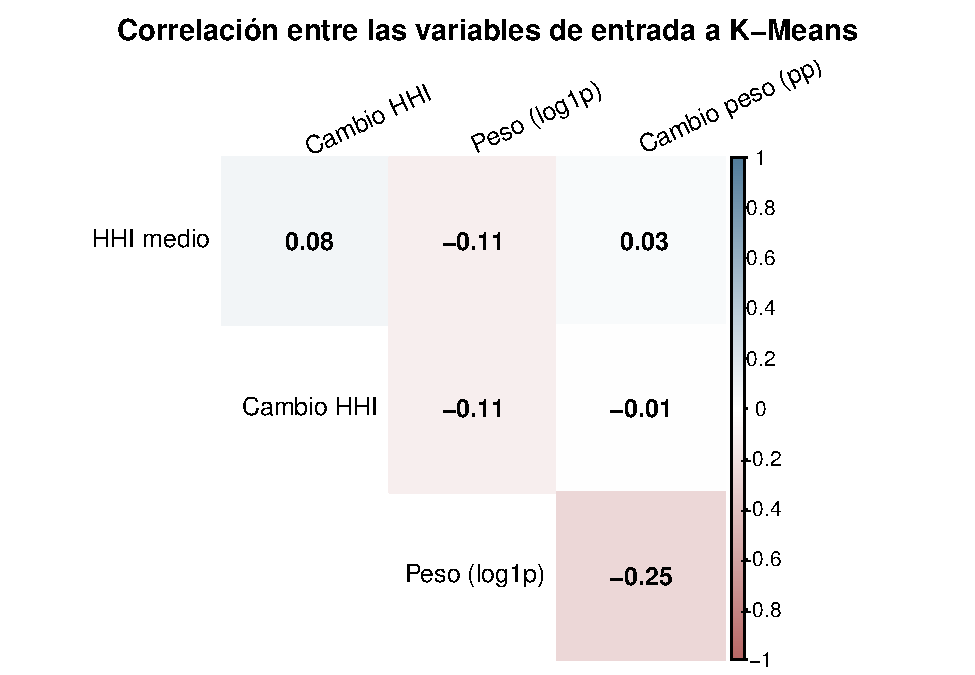
\includegraphics{Proyecto_9_EDA_files/Proyecto_9_EDA_files/figure-latex/unnamed-chunk-13-1.pdf}
La tabla de momentos estadísticos muestra que en la participación media
(\%), la media (1.001 \%) es mucho mayor que la mediana (0.203 \%), la
asimetría de 4.9 y la curtosis 25.5. Esto ocurre porque la distribución
tiene una cola derecha extrema: tan solo dos capítulos (HS85 y HS84)
concentran cerca del 39 \% de las importaciones, mientras que la mayoría
de los capítulos representa menos del 0.5 \% cada uno.

Al aplicar peso\_log = log1p(100 * participacion\_media), la asimetría y
la curtosis se reducen drásticamente. Esto demuestra por qué fue
necesario transformar la variable: si metiéramos la participación cruda
a K-Means, la distancia euclidiana estaría dominada únicamente por HS85
y HS84.

En HHI, tanto la media como la mediana son ligeramente negativas,
reflejando un proceso generalizado de diversificación comercial, es
decir, esta reducción responde a una menor dependencia del proveedor
principal (top1) y a una menor asimetría en las cuotas de abastecimiento
dentro de la mayoría de los capítulos.

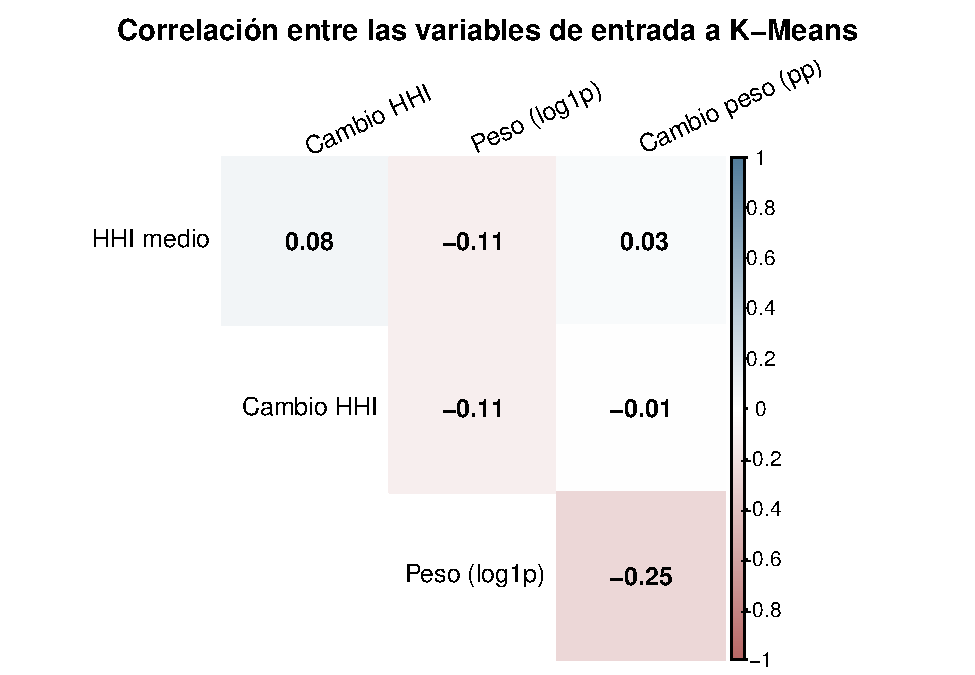
\includegraphics{Proyecto_9_EDA_files/Proyecto_9_EDA_files/figure-latex/unnamed-chunk-14-1.pdf}

La matriz de correlación indica que las relaciones lineales entre las
cuatro variables de entrada son bajas o moderadas (ningún coeficiente
supera \(\vert{}r\vert{} = 0.45\)). En particular, la correlación
cercana a cero entre \texttt{Peso\ (log1p)} y \texttt{HHI\ medio}
confirma que los capítulos donde México gasta más dinero no son
necesariamente los más concentrados en un solo proveedo, por lo tanto,
que no existan valores altos (\textgreater.80) valida que las cuatro
variables aportan información distinta y no redundante al algoritmo
K-Means.

El siguiente paso es ajustar varios números de grupos, comparar su
separación e interpretar qué capítulos quedaron en cada uno.

\begin{verbatim}
## tibble [96 x 7] (S3: tbl_df/tbl/data.frame)
##  $ hs2                : chr [1:96] "01" "02" "03" "04" ...
##  $ capitulo           : chr [1:96] "Animals; live" "Meat and edible meat offal" "Fish and crustaceans, molluscs and other aquatic invertebrates" "Dairy produce; birds' eggs; natural honey; edible products of animal origin, not elsewhere specified or included" ...
##  $ hhi_medio          : num [1:96] 0.523 0.641 0.22 0.658 0.694 ...
##  $ cambio_hhi         : num [1:96] -0.0176 -0.147 0.0716 0.1002 -0.1792 ...
##  $ participacion_media: num [1:96] 0.000409 0.010472 0.001417 0.00465 0.000608 ...
##  $ cambio_peso_pp     : num [1:96] -0.01588 0.31769 -0.01385 0.05967 -0.00297 ...
##  $ peso_log           : num [1:96] 0.0401 0.7165 0.1325 0.3819 0.059 ...
\end{verbatim}

Para determinar el número de grupos a utilizar en K-Means, se evaluaron
soluciones entre (K=2) y (K=8). Para cada alternativa se calcularon dos
métricas: la suma de cuadrados dentro de los clusters (WSS), que mide la
dispersión interna de los grupos, y el coeficiente silhouette promedio,
que evalúa qué tan bien separadas se encuentran las observaciones entre
clusters.

\begin{longtable}[]{@{}rrr@{}}
\caption{Evaluación del número de clusters}\tabularnewline
\toprule\noalign{}
k & wss & silhouette \\
\midrule\noalign{}
\endfirsthead
\toprule\noalign{}
k & wss & silhouette \\
\midrule\noalign{}
\endhead
\bottomrule\noalign{}
\endlastfoot
2 & 285.356 & 0.511 \\
3 & 215.920 & 0.382 \\
4 & 165.116 & 0.318 \\
5 & 124.508 & 0.349 \\
6 & 107.049 & 0.302 \\
7 & 95.836 & 0.306 \\
8 & 86.067 & 0.308 \\
\end{longtable}

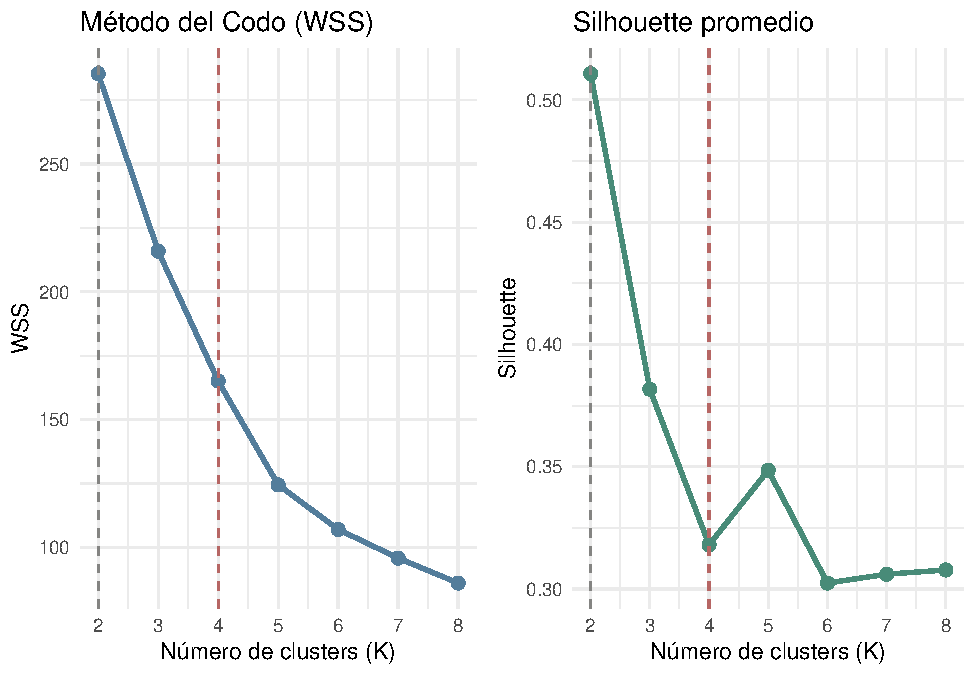
\includegraphics{Proyecto_9_EDA_files/Proyecto_9_EDA_files/figure-latex/unnamed-chunk-16-1.pdf}

La WSS disminuye conforme aumenta el número de clusters, comportamiento
esperado en K-Means debido a que una mayor cantidad de grupos permite
reducir la variabilidad interna. Por ello, esta métrica no debe
interpretarse de manera aislada.

El valor más alto de silhouette se obtuvo con (K=2), con un valor de
0.511, superior al observado para las demás alternativas. Esto sugiere
que la solución de dos clusters presenta la mejor separación relativa
entre grupos dentro de las opciones evaluadas.

Por esta razón, se seleccionó inicialmente (K=2) para ajustar el modelo
final. No obstante, además del criterio estadístico, se revisará la
composición y el perfil de los clusters para verificar que la solución
tenga una interpretación económica adecuada.

\begin{verbatim}
## 
##  1  2 
##  7 89
\end{verbatim}

\begin{verbatim}
##      hhi_medio   cambio_hhi   peso_log cambio_peso_pp
## 1 -0.109625529  0.062836053  2.6660474     -2.3261335
## 2  0.008622233 -0.004942161 -0.2096891      0.1829543
\end{verbatim}

El modelo K-Means con (K=2) generó dos grupos de tamaños muy distintos:
el cluster 1 contiene 7 capítulos HS2, mientras que el cluster 2
contiene 89 capítulos. Esta diferencia en tamaño no implica por sí misma
que el agrupamiento sea incorrecto. Sin embargo, sugiere que el
algoritmo está identificando un conjunto reducido de capítulos con
características considerablemente distintas respecto al resto de las
importaciones. Por ello, antes de interpretar los grupos como perfiles
económicos definitivos, es necesario revisar qué capítulos integran cada
cluster y cuáles variables explican principalmente esta separación.

Los centroides estandarizados muestran que la principal diferencia entre
los dos clusters se encuentra en el peso económico de los capítulos. El
cluster 1 presenta un valor de peso\_log considerablemente superior al
promedio, mientras que el cluster 2 se encuentra ligeramente por debajo.

El cluster 1 también presenta, en promedio, una reducción relativa en su
participación dentro de las importaciones y un aumento ligeramente mayor
de la concentración de proveedores. En contraste, el cluster 2 reúne a
la mayoría de los capítulos y presenta valores más cercanos al promedio
general.

Debido a que los centroides se encuentran expresados en unidades
estandarizadas, estos valores muestran diferencias relativas respecto al
promedio y no deben interpretarse directamente como porcentajes de
participación o puntos del índice HHI, por lo que a continuación se
examina la composición de cada grupo y su perfil promedio en escala
original

\begin{longtable}[]{@{}
  >{\raggedright\arraybackslash}p{(\columnwidth - 12\tabcolsep) * \real{0.0265}}
  >{\raggedright\arraybackslash}p{(\columnwidth - 12\tabcolsep) * \real{0.0132}}
  >{\raggedright\arraybackslash}p{(\columnwidth - 12\tabcolsep) * \real{0.7748}}
  >{\raggedleft\arraybackslash}p{(\columnwidth - 12\tabcolsep) * \real{0.0331}}
  >{\raggedleft\arraybackslash}p{(\columnwidth - 12\tabcolsep) * \real{0.0364}}
  >{\raggedleft\arraybackslash}p{(\columnwidth - 12\tabcolsep) * \real{0.0662}}
  >{\raggedleft\arraybackslash}p{(\columnwidth - 12\tabcolsep) * \real{0.0497}}@{}}
\caption{Capítulos HS2 asignados a cada cluster}\tabularnewline
\toprule\noalign{}
\begin{minipage}[b]{\linewidth}\raggedright
cluster
\end{minipage} & \begin{minipage}[b]{\linewidth}\raggedright
hs2
\end{minipage} & \begin{minipage}[b]{\linewidth}\raggedright
capitulo
\end{minipage} & \begin{minipage}[b]{\linewidth}\raggedleft
hhi\_medio
\end{minipage} & \begin{minipage}[b]{\linewidth}\raggedleft
cambio\_hhi
\end{minipage} & \begin{minipage}[b]{\linewidth}\raggedleft
participacion\_media
\end{minipage} & \begin{minipage}[b]{\linewidth}\raggedleft
cambio\_peso\_pp
\end{minipage} \\
\midrule\noalign{}
\endfirsthead
\toprule\noalign{}
\begin{minipage}[b]{\linewidth}\raggedright
cluster
\end{minipage} & \begin{minipage}[b]{\linewidth}\raggedright
hs2
\end{minipage} & \begin{minipage}[b]{\linewidth}\raggedright
capitulo
\end{minipage} & \begin{minipage}[b]{\linewidth}\raggedleft
hhi\_medio
\end{minipage} & \begin{minipage}[b]{\linewidth}\raggedleft
cambio\_hhi
\end{minipage} & \begin{minipage}[b]{\linewidth}\raggedleft
participacion\_media
\end{minipage} & \begin{minipage}[b]{\linewidth}\raggedleft
cambio\_peso\_pp
\end{minipage} \\
\midrule\noalign{}
\endhead
\bottomrule\noalign{}
\endlastfoot
1 & 85 & Electrical machinery and equipment and parts thereof; sound
recorders and reproducers; television image and sound recorders and
reproducers, parts and accessories of such articles & 0.203 & -0.030 &
0.202 & -0.718 \\
1 & 84 & Machinery and mechanical appliances, boilers, nuclear reactors;
parts thereof & 0.208 & -0.031 & 0.167 & -0.266 \\
1 & 27 & Mineral fuels, mineral oils and products of their distillation;
bituminous substances; mineral waxes & 0.815 & 0.100 & 0.080 & -0.280 \\
1 & 39 & Plastics and articles thereof & 0.445 & -0.074 & 0.055 &
-0.581 \\
1 & 90 & Optical, photographic, cinematographic, measuring, checking,
medical or surgical instruments and apparatus; parts and accessories &
0.232 & 0.021 & 0.034 & -0.727 \\
1 & 73 & Iron or steel articles & 0.309 & -0.036 & 0.020 & -0.393 \\
1 & 29 & Organic chemicals & 0.373 & 0.023 & 0.020 & -0.302 \\
2 & 87 & Vehicles; other than railway or tramway rolling stock, and
parts and accessories thereof & 0.255 & -0.061 & 0.095 & 0.612 \\
2 & 72 & Iron and steel & 0.209 & -0.056 & 0.028 & 0.811 \\
2 & 76 & Aluminium and articles thereof & 0.250 & -0.105 & 0.016 &
0.251 \\
2 & 40 & Rubber and articles thereof & 0.242 & -0.033 & 0.015 &
-0.207 \\
2 & 38 & Chemical products n.e.c. & 0.415 & -0.059 & 0.013 & 0.272 \\
2 & 48 & Paper and paperboard; articles of paper pulp, of paper or
paperboard & 0.463 & -0.159 & 0.013 & -0.271 \\
2 & 10 & Cereals & 0.757 & 0.041 & 0.012 & 0.231 \\
2 & 30 & Pharmaceutical products & 0.125 & -0.025 & 0.012 & 0.321 \\
2 & 02 & Meat and edible meat offal & 0.641 & -0.147 & 0.010 & 0.318 \\
2 & 12 & Oil seeds and oleaginous fruits; miscellaneous grains, seeds
and fruit, industrial or medicinal plants; straw and fodder & 0.411 &
-0.033 & 0.009 & 0.063 \\
2 & 94 & Furniture; bedding, mattresses, mattress supports, cushions and
similar stuffed furnishings; lamps and lighting fittings, n.e.c.;
illuminated signs, illuminated name-plates and the like; prefabricated
buildings & 0.291 & -0.016 & 0.008 & -0.194 \\
2 & 33 & Essential oils and resinoids; perfumery, cosmetic or toilet
preparations & 0.230 & -0.004 & 0.008 & 0.129 \\
2 & 74 & Copper and articles thereof & 0.525 & -0.149 & 0.008 & 0.150 \\
2 & 28 & Inorganic chemicals; organic and inorganic compounds of
precious metals; of rare earth metals, of radio-active elements and of
isotopes & 0.479 & 0.033 & 0.006 & -0.003 \\
2 & 83 & Metal; miscellaneous products of base metal & 0.287 & -0.050 &
0.006 & -0.089 \\
2 & 32 & Tanning or dyeing extracts; tannins and their derivatives;
dyes, pigments and other colouring matter; paints, varnishes; putty,
other mastics; inks & 0.371 & -0.050 & 0.005 & -0.087 \\
2 & 61 & Apparel and clothing accessories; knitted or crocheted & 0.154
& 0.039 & 0.005 & 0.178 \\
2 & 95 & Toys, games and sports requisites; parts and accessories
thereof & 0.490 & -0.169 & 0.005 & -0.001 \\
2 & 82 & Tools, implements, cutlery, spoons and forks, of base metal;
parts thereof, of base metal & 0.179 & -0.005 & 0.005 & -0.116 \\
2 & 04 & Dairy produce; birds' eggs; natural honey; edible products of
animal origin, not elsewhere specified or included & 0.658 & 0.100 &
0.005 & 0.060 \\
2 & 44 & Wood and articles of wood; wood charcoal & 0.225 & -0.021 &
0.004 & -0.037 \\
2 & 62 & Apparel and clothing accessories; not knitted or crocheted &
0.179 & -0.014 & 0.004 & 0.056 \\
2 & 23 & Food industries, residues and wastes thereof; prepared animal
fodder & 0.829 & -0.048 & 0.004 & -0.011 \\
2 & 31 & Fertilizers & 0.146 & 0.017 & 0.004 & 0.016 \\
2 & 21 & Miscellaneous edible preparations & 0.656 & -0.069 & 0.004 &
0.049 \\
2 & 70 & Glass and glassware & 0.340 & -0.049 & 0.003 & -0.028 \\
2 & 15 & Animal, vegetable or microbial fats and oils and their cleavage
products; prepared edible fats; animal or vegetable waxes & 0.186 &
-0.143 & 0.003 & 0.008 \\
2 & 64 & Footwear; gaiters and the like; parts of such articles & 0.254
& 0.000 & 0.003 & 0.079 \\
2 & 08 & Fruit and nuts, edible; peel of citrus fruit or melons & 0.638
& -0.123 & 0.003 & 0.063 \\
2 & 26 & Ores, slag and ash & 0.400 & 0.364 & 0.003 & 0.144 \\
2 & 86 & Railway, tramway locomotives, rolling-stock and parts thereof;
railway or tramway track fixtures and fittings and parts thereof;
mechanical (including electro-mechanical) traffic signalling equipment
of all kinds & 0.568 & -0.113 & 0.003 & -0.044 \\
2 & 71 & Natural, cultured pearls; precious, semi-precious stones;
precious metals, metals clad with precious metal, and articles thereof;
imitation jewellery; coin & 0.239 & -0.163 & 0.003 & 0.026 \\
2 & 34 & Soap, organic surface-active agents; washing, lubricating,
polishing or scouring preparations; artificial or prepared waxes,
candles and similar articles, modelling pastes, dental waxes and dental
preparations with a basis of plaster & 0.441 & -0.100 & 0.002 & 0.002 \\
2 & 47 & Pulp of wood or other fibrous cellulosic material; recovered
(waste and scrap) paper or paperboard & 0.552 & -0.041 & 0.002 &
-0.036 \\
2 & 22 & Beverages, spirits and vinegar & 0.227 & -0.017 & 0.002 &
-0.075 \\
2 & 54 & Man-made filaments; strip and the like of man-made textile
materials & 0.276 & -0.015 & 0.002 & -0.055 \\
2 & 59 & Textile fabrics; impregnated, coated, covered or laminated;
textile articles of a kind suitable for industrial use & 0.449 & -0.215
& 0.002 & -0.091 \\
2 & 35 & Albuminoidal substances; modified starches; glues; enzymes &
0.277 & -0.072 & 0.002 & -0.005 \\
2 & 96 & Miscellaneous manufactured articles & 0.258 & 0.050 & 0.002 &
-0.029 \\
2 & 17 & Sugars and sugar confectionery & 0.704 & -0.167 & 0.002 &
0.049 \\
2 & 42 & Articles of leather; saddlery and harness; travel goods,
handbags and similar containers; articles of animal gut (other than
silk-worm gut) & 0.323 & -0.074 & 0.002 & -0.009 \\
2 & 20 & Preparations of vegetables, fruit, nuts or other parts of
plants & 0.375 & -0.078 & 0.002 & 0.058 \\
2 & 69 & Ceramic products & 0.200 & -0.025 & 0.002 & -0.024 \\
2 & 52 & Cotton & 0.515 & -0.133 & 0.002 & -0.134 \\
2 & 63 & Textiles, made up articles; sets; worn clothing and worn
textile articles; rags & 0.339 & 0.044 & 0.002 & 0.046 \\
2 & 56 & Wadding, felt and nonwovens, special yarns; twine, cordage,
ropes and cables and articles thereof & 0.446 & -0.236 & 0.002 &
-0.044 \\
2 & 68 & Stone, plaster, cement, asbestos, mica or similar materials;
articles thereof & 0.210 & -0.026 & 0.002 & -0.036 \\
2 & 41 & Raw hides and skins (other than furskins) and leather & 0.203 &
0.019 & 0.002 & -0.190 \\
2 & 19 & Preparations of cereals, flour, starch or milk; pastrycooks'
products & 0.354 & -0.046 & 0.002 & 0.036 \\
2 & 55 & Man-made staple fibres & 0.302 & -0.041 & 0.001 & -0.071 \\
2 & 11 & Products of the milling industry; malt, starches, inulin, wheat
gluten & 0.494 & -0.167 & 0.001 & 0.001 \\
2 & 60 & Fabrics; knitted or crocheted & 0.396 & 0.015 & 0.001 &
-0.070 \\
2 & 49 & Printed books, newspapers, pictures and other products of the
printing industry; manuscripts, typescripts and plans & 0.409 & -0.036 &
0.001 & -0.059 \\
2 & 25 & Salt; sulphur; earths, stone; plastering materials, lime and
cement & 0.373 & -0.043 & 0.001 & -0.017 \\
2 & 03 & Fish and crustaceans, molluscs and other aquatic invertebrates
& 0.220 & 0.072 & 0.001 & -0.014 \\
2 & 07 & Vegetables and certain roots and tubers; edible & 0.578 & 0.001
& 0.001 & 0.068 \\
2 & 18 & Cocoa and cocoa preparations & 0.209 & -0.081 & 0.001 &
0.036 \\
2 & 16 & Meat, fish, crustaceans, molluscs or other aquatic
invertebrates, or insects; preparations thereof & 0.517 & 0.130 & 0.001
& 0.001 \\
2 & 09 & Coffee, tea, mate and spices & 0.136 & 0.028 & 0.001 & 0.006 \\
2 & 81 & Metals; n.e.c., cermets and articles thereof & 0.345 & 0.018 &
0.001 & -0.007 \\
2 & 91 & Clocks and watches and parts thereof & 0.448 & 0.191 & 0.001 &
-0.006 \\
2 & 58 & Fabrics; special woven fabrics, tufted textile fabrics, lace,
tapestries, trimmings, embroidery & 0.252 & -0.018 & 0.001 & -0.029 \\
2 & 75 & Nickel and articles thereof & 0.395 & 0.121 & 0.001 & 0.022 \\
2 & 05 & Animal originated products; not elsewhere specified or included
& 0.694 & -0.179 & 0.001 & -0.003 \\
2 & 88 & Aircraft, spacecraft, and parts thereof & 0.458 & -0.077 &
0.001 & -0.001 \\
2 & 37 & Photographic or cinematographic goods & 0.349 & -0.147 & 0.001
& -0.051 \\
2 & 79 & Zinc and articles thereof & 0.386 & -0.202 & 0.000 & 0.007 \\
2 & 65 & Headgear and parts thereof & 0.425 & -0.095 & 0.000 & 0.019 \\
2 & 57 & Carpets and other textile floor coverings & 0.326 & -0.216 &
0.000 & -0.011 \\
2 & 01 & Animals; live & 0.523 & -0.018 & 0.000 & -0.016 \\
2 & 36 & Explosives; pyrotechnic products; matches; pyrophoric alloys;
certain combustible preparations & 0.419 & -0.095 & 0.000 & -0.035 \\
2 & 13 & Lac; gums, resins and other vegetable saps and extracts & 0.140
& -0.012 & 0.000 & -0.001 \\
2 & 06 & Trees and other plants, live; bulbs, roots and the like; cut
flowers and ornamental foliage & 0.456 & 0.030 & 0.000 & 0.002 \\
2 & 80 & Tin; articles thereof & 0.199 & 0.070 & 0.000 & -0.007 \\
2 & 89 & Ships, boats and floating structures & 0.577 & 0.255 & 0.000 &
-0.003 \\
2 & 92 & Musical instruments; parts and accessories of such articles &
0.342 & -0.004 & 0.000 & -0.001 \\
2 & 24 & Tobacco and manufactured tobacco substitutes; products, whether
or not containing nicotine, intended for inhalation without combustion;
other nicotine containing products intended for the intake of nicotine
into the human body & 0.711 & 0.454 & 0.000 & -0.016 \\
2 & 78 & Lead and articles thereof & 0.691 & 0.040 & 0.000 & -0.002 \\
2 & 67 & Feathers and down, prepared; and articles made of feather or of
down; artificial flowers; articles of human hair & 0.802 & 0.237 & 0.000
& 0.001 \\
2 & 51 & Wool, fine or coarse animal hair; horsehair yarn and woven
fabric & 0.220 & 0.067 & 0.000 & -0.013 \\
2 & 45 & Cork and articles of cork & 0.531 & -0.009 & 0.000 & 0.004 \\
2 & 93 & Arms and ammunition; parts and accessories thereof & 0.384 &
0.274 & 0.000 & -0.005 \\
2 & 97 & Works of art; collectors' pieces and antiques & 0.207 & 0.083 &
0.000 & -0.013 \\
2 & 66 & Umbrellas, sun umbrellas, walking-sticks, seat sticks, whips,
riding crops; and parts thereof & 0.779 & -0.016 & 0.000 & -0.002 \\
2 & 53 & Vegetable textile fibres; paper yarn and woven fabrics of paper
yarn & 0.303 & 0.013 & 0.000 & -0.005 \\
2 & 14 & Vegetable plaiting materials; vegetable products not elsewhere
specified or included & 0.357 & 0.357 & 0.000 & 0.005 \\
2 & 46 & Manufactures of straw, esparto or other plaiting materials;
basketware and wickerwork & 0.421 & -0.100 & 0.000 & 0.002 \\
2 & 43 & Furskins and artificial fur; manufactures thereof & 0.248 &
0.039 & 0.000 & -0.001 \\
2 & 50 & Silk & 0.464 & 0.354 & 0.000 & 0.000 \\
\end{longtable}

La solución con \(K=2\) asignó \textbf{7 capítulos al cluster 1 y 89 al
cluster 2}. El primer grupo está integrado por equipo eléctrico (HS85),
maquinaria mecánica (HS84), combustibles minerales (HS27), plásticos
(HS39), instrumentos ópticos y médicos (HS90), artículos de hierro o
acero (HS73) y productos químicos orgánicos (HS29).

Los capítulos del cluster 1 se caracterizan principalmente por tener una
participación relativamente elevada dentro de las importaciones
mexicanas y, en todos los casos, por haber reducido su participación
entre el periodo inicial y final considerados. Sin embargo, no presentan
un nivel homogéneo de concentración de proveedores: su HHI medio varía
considerablemente entre capítulos.

Por lo tanto, la separación obtenida con \(K=2\) parece estar
determinada en mayor medida por la importancia económica y su cambio en
el tiempo que por un patrón común de concentración. Esto debe
considerarse al interpretar los clusters, ya que el objetivo del
análisis es estudiar conjuntamente ambas dimensiones.

\begin{longtable}[]{@{}
  >{\raggedright\arraybackslash}p{(\columnwidth - 10\tabcolsep) * \real{0.1026}}
  >{\raggedleft\arraybackslash}p{(\columnwidth - 10\tabcolsep) * \real{0.1282}}
  >{\raggedleft\arraybackslash}p{(\columnwidth - 10\tabcolsep) * \real{0.1282}}
  >{\raggedleft\arraybackslash}p{(\columnwidth - 10\tabcolsep) * \real{0.1410}}
  >{\raggedleft\arraybackslash}p{(\columnwidth - 10\tabcolsep) * \real{0.3077}}
  >{\raggedleft\arraybackslash}p{(\columnwidth - 10\tabcolsep) * \real{0.1923}}@{}}
\caption{Perfil promedio de los clusters en unidades
originales}\tabularnewline
\toprule\noalign{}
\begin{minipage}[b]{\linewidth}\raggedright
cluster
\end{minipage} & \begin{minipage}[b]{\linewidth}\raggedleft
capitulos
\end{minipage} & \begin{minipage}[b]{\linewidth}\raggedleft
hhi\_medio
\end{minipage} & \begin{minipage}[b]{\linewidth}\raggedleft
cambio\_hhi
\end{minipage} & \begin{minipage}[b]{\linewidth}\raggedleft
participacion\_media\_pct
\end{minipage} & \begin{minipage}[b]{\linewidth}\raggedleft
cambio\_peso\_pp
\end{minipage} \\
\midrule\noalign{}
\endfirsthead
\toprule\noalign{}
\begin{minipage}[b]{\linewidth}\raggedright
cluster
\end{minipage} & \begin{minipage}[b]{\linewidth}\raggedleft
capitulos
\end{minipage} & \begin{minipage}[b]{\linewidth}\raggedleft
hhi\_medio
\end{minipage} & \begin{minipage}[b]{\linewidth}\raggedleft
cambio\_hhi
\end{minipage} & \begin{minipage}[b]{\linewidth}\raggedleft
participacion\_media\_pct
\end{minipage} & \begin{minipage}[b]{\linewidth}\raggedleft
cambio\_peso\_pp
\end{minipage} \\
\midrule\noalign{}
\endhead
\bottomrule\noalign{}
\endlastfoot
1 & 7 & 0.369 & -0.004 & 8.266 & -0.467 \\
2 & 89 & 0.390 & -0.013 & 0.429 & 0.022 \\
\end{longtable}

La comparación de los perfiles promedio muestra que la principal
diferencia entre los dos clusters corresponde al peso económico de los
capítulos dentro de las importaciones mexicanas. Los siete capítulos del
cluster 1 representan, en promedio, 8.27\% de las importaciones,
mientras que los 89 capítulos del cluster 2 representan aproximadamente
0.43\%.

En contraste, los niveles medios de concentración son similares entre
ambos grupos: el HHI promedio es 0.369 en el cluster 1 y 0.390 en el
cluster 2. Asimismo, los cambios promedio del HHI son relativamente
pequeños en ambos casos.

Por lo tanto, aunque (K=2) presenta la mayor silhouette promedio entre
las alternativas evaluadas, la separación obtenida está determinada
principalmente por la importancia económica de los capítulos y no genera
una diferenciación clara en términos de concentración de proveedores.
Debido a ello, resulta conveniente analizar también una solución con un
mayor número de clusters antes de seleccionar el modelo definitivo.

Por lo tanto, replicamos el procedimiento anterior utilizando \(K=4\)
para evaluar si un mayor número de grupos permite separar los capítulos
tanto por su peso económico como por su nivel y cambio de concentración.

\begin{verbatim}
## 
##  1  2  3  4 
##  7 46 32 11
\end{verbatim}

\begin{longtable}[]{@{}rrrr@{}}
\caption{Centroides en variables estandarizadas (K = 4)}\tabularnewline
\toprule\noalign{}
hhi\_medio & cambio\_hhi & peso\_log & cambio\_peso\_pp \\
\midrule\noalign{}
\endfirsthead
\toprule\noalign{}
hhi\_medio & cambio\_hhi & peso\_log & cambio\_peso\_pp \\
\midrule\noalign{}
\endhead
\bottomrule\noalign{}
\endlastfoot
-0.110 & 0.063 & 2.666 & -2.326 \\
-0.738 & -0.055 & -0.077 & 0.247 \\
0.829 & -0.668 & -0.295 & 0.096 \\
0.743 & 2.136 & -0.517 & 0.167 \\
\end{longtable}

A diferencia de \(K=2\) (donde solo peso\_log y cambio\_peso\_pp se
alejaban de cero mientras hhi\_medio quedaba casi en 0 en ambos grupos),
en la tabla de centroides de \(K=4\) cada grupo se especializa en una
dimensión distinta:

\begin{enumerate}
\def\labelenumi{\arabic{enumi}.}
\tightlist
\item
  Este grupo tiene el centroide con peso\_log muy elevado (es decir,
  capítulos gigantes de las importaciones mexicanas).\\
\item
  Otro grupo destaca por tener el centroide con hhi\_medio altamente
  positivo y/o cambio\_hhi positivo (capítulos de alta concentración).\\
\item
  Un tercer grupo presenta cambio\_hhi marcadamente negativo (capítulos
  que redujeron su concentración y diversificaron proveedores).\\
\item
  El ultimo grupo agrupa a los capítulos de peso pequeño/intermedio y
  estabilidad relativa (valores cercanos al promedio 0 en cambio de peso
  y concentración moderada).
\end{enumerate}

Una vez revisados los centroides estandarizados, asignamos a cada
capítulo HS2 su número de cluster correspondiente en
\texttt{datos\_clusters4} y los ordenamos de mayor a menor participación
media dentro de cada grupo para identificar qué sectores concretos
integran cada perfil:

\begin{longtable}[]{@{}
  >{\raggedright\arraybackslash}p{(\columnwidth - 12\tabcolsep) * \real{0.0265}}
  >{\raggedright\arraybackslash}p{(\columnwidth - 12\tabcolsep) * \real{0.0132}}
  >{\raggedright\arraybackslash}p{(\columnwidth - 12\tabcolsep) * \real{0.7748}}
  >{\raggedleft\arraybackslash}p{(\columnwidth - 12\tabcolsep) * \real{0.0331}}
  >{\raggedleft\arraybackslash}p{(\columnwidth - 12\tabcolsep) * \real{0.0364}}
  >{\raggedleft\arraybackslash}p{(\columnwidth - 12\tabcolsep) * \real{0.0662}}
  >{\raggedleft\arraybackslash}p{(\columnwidth - 12\tabcolsep) * \real{0.0497}}@{}}
\caption{Capítulos HS2 asignados a cada cluster (k=4)}\tabularnewline
\toprule\noalign{}
\begin{minipage}[b]{\linewidth}\raggedright
cluster
\end{minipage} & \begin{minipage}[b]{\linewidth}\raggedright
hs2
\end{minipage} & \begin{minipage}[b]{\linewidth}\raggedright
capitulo
\end{minipage} & \begin{minipage}[b]{\linewidth}\raggedleft
hhi\_medio
\end{minipage} & \begin{minipage}[b]{\linewidth}\raggedleft
cambio\_hhi
\end{minipage} & \begin{minipage}[b]{\linewidth}\raggedleft
participacion\_media
\end{minipage} & \begin{minipage}[b]{\linewidth}\raggedleft
cambio\_peso\_pp
\end{minipage} \\
\midrule\noalign{}
\endfirsthead
\toprule\noalign{}
\begin{minipage}[b]{\linewidth}\raggedright
cluster
\end{minipage} & \begin{minipage}[b]{\linewidth}\raggedright
hs2
\end{minipage} & \begin{minipage}[b]{\linewidth}\raggedright
capitulo
\end{minipage} & \begin{minipage}[b]{\linewidth}\raggedleft
hhi\_medio
\end{minipage} & \begin{minipage}[b]{\linewidth}\raggedleft
cambio\_hhi
\end{minipage} & \begin{minipage}[b]{\linewidth}\raggedleft
participacion\_media
\end{minipage} & \begin{minipage}[b]{\linewidth}\raggedleft
cambio\_peso\_pp
\end{minipage} \\
\midrule\noalign{}
\endhead
\bottomrule\noalign{}
\endlastfoot
1 & 85 & Electrical machinery and equipment and parts thereof; sound
recorders and reproducers; television image and sound recorders and
reproducers, parts and accessories of such articles & 0.203 & -0.030 &
0.202 & -0.718 \\
1 & 84 & Machinery and mechanical appliances, boilers, nuclear reactors;
parts thereof & 0.208 & -0.031 & 0.167 & -0.266 \\
1 & 27 & Mineral fuels, mineral oils and products of their distillation;
bituminous substances; mineral waxes & 0.815 & 0.100 & 0.080 & -0.280 \\
1 & 39 & Plastics and articles thereof & 0.445 & -0.074 & 0.055 &
-0.581 \\
1 & 90 & Optical, photographic, cinematographic, measuring, checking,
medical or surgical instruments and apparatus; parts and accessories &
0.232 & 0.021 & 0.034 & -0.727 \\
1 & 73 & Iron or steel articles & 0.309 & -0.036 & 0.020 & -0.393 \\
1 & 29 & Organic chemicals & 0.373 & 0.023 & 0.020 & -0.302 \\
2 & 87 & Vehicles; other than railway or tramway rolling stock, and
parts and accessories thereof & 0.255 & -0.061 & 0.095 & 0.612 \\
2 & 72 & Iron and steel & 0.209 & -0.056 & 0.028 & 0.811 \\
2 & 76 & Aluminium and articles thereof & 0.250 & -0.105 & 0.016 &
0.251 \\
2 & 40 & Rubber and articles thereof & 0.242 & -0.033 & 0.015 &
-0.207 \\
2 & 38 & Chemical products n.e.c. & 0.415 & -0.059 & 0.013 & 0.272 \\
2 & 30 & Pharmaceutical products & 0.125 & -0.025 & 0.012 & 0.321 \\
2 & 12 & Oil seeds and oleaginous fruits; miscellaneous grains, seeds
and fruit, industrial or medicinal plants; straw and fodder & 0.411 &
-0.033 & 0.009 & 0.063 \\
2 & 94 & Furniture; bedding, mattresses, mattress supports, cushions and
similar stuffed furnishings; lamps and lighting fittings, n.e.c.;
illuminated signs, illuminated name-plates and the like; prefabricated
buildings & 0.291 & -0.016 & 0.008 & -0.194 \\
2 & 33 & Essential oils and resinoids; perfumery, cosmetic or toilet
preparations & 0.230 & -0.004 & 0.008 & 0.129 \\
2 & 83 & Metal; miscellaneous products of base metal & 0.287 & -0.050 &
0.006 & -0.089 \\
2 & 32 & Tanning or dyeing extracts; tannins and their derivatives;
dyes, pigments and other colouring matter; paints, varnishes; putty,
other mastics; inks & 0.371 & -0.050 & 0.005 & -0.087 \\
2 & 61 & Apparel and clothing accessories; knitted or crocheted & 0.154
& 0.039 & 0.005 & 0.178 \\
2 & 82 & Tools, implements, cutlery, spoons and forks, of base metal;
parts thereof, of base metal & 0.179 & -0.005 & 0.005 & -0.116 \\
2 & 44 & Wood and articles of wood; wood charcoal & 0.225 & -0.021 &
0.004 & -0.037 \\
2 & 62 & Apparel and clothing accessories; not knitted or crocheted &
0.179 & -0.014 & 0.004 & 0.056 \\
2 & 31 & Fertilizers & 0.146 & 0.017 & 0.004 & 0.016 \\
2 & 70 & Glass and glassware & 0.340 & -0.049 & 0.003 & -0.028 \\
2 & 15 & Animal, vegetable or microbial fats and oils and their cleavage
products; prepared edible fats; animal or vegetable waxes & 0.186 &
-0.143 & 0.003 & 0.008 \\
2 & 64 & Footwear; gaiters and the like; parts of such articles & 0.254
& 0.000 & 0.003 & 0.079 \\
2 & 71 & Natural, cultured pearls; precious, semi-precious stones;
precious metals, metals clad with precious metal, and articles thereof;
imitation jewellery; coin & 0.239 & -0.163 & 0.003 & 0.026 \\
2 & 22 & Beverages, spirits and vinegar & 0.227 & -0.017 & 0.002 &
-0.075 \\
2 & 54 & Man-made filaments; strip and the like of man-made textile
materials & 0.276 & -0.015 & 0.002 & -0.055 \\
2 & 35 & Albuminoidal substances; modified starches; glues; enzymes &
0.277 & -0.072 & 0.002 & -0.005 \\
2 & 96 & Miscellaneous manufactured articles & 0.258 & 0.050 & 0.002 &
-0.029 \\
2 & 42 & Articles of leather; saddlery and harness; travel goods,
handbags and similar containers; articles of animal gut (other than
silk-worm gut) & 0.323 & -0.074 & 0.002 & -0.009 \\
2 & 20 & Preparations of vegetables, fruit, nuts or other parts of
plants & 0.375 & -0.078 & 0.002 & 0.058 \\
2 & 69 & Ceramic products & 0.200 & -0.025 & 0.002 & -0.024 \\
2 & 63 & Textiles, made up articles; sets; worn clothing and worn
textile articles; rags & 0.339 & 0.044 & 0.002 & 0.046 \\
2 & 68 & Stone, plaster, cement, asbestos, mica or similar materials;
articles thereof & 0.210 & -0.026 & 0.002 & -0.036 \\
2 & 41 & Raw hides and skins (other than furskins) and leather & 0.203 &
0.019 & 0.002 & -0.190 \\
2 & 19 & Preparations of cereals, flour, starch or milk; pastrycooks'
products & 0.354 & -0.046 & 0.002 & 0.036 \\
2 & 55 & Man-made staple fibres & 0.302 & -0.041 & 0.001 & -0.071 \\
2 & 60 & Fabrics; knitted or crocheted & 0.396 & 0.015 & 0.001 &
-0.070 \\
2 & 25 & Salt; sulphur; earths, stone; plastering materials, lime and
cement & 0.373 & -0.043 & 0.001 & -0.017 \\
2 & 03 & Fish and crustaceans, molluscs and other aquatic invertebrates
& 0.220 & 0.072 & 0.001 & -0.014 \\
2 & 18 & Cocoa and cocoa preparations & 0.209 & -0.081 & 0.001 &
0.036 \\
2 & 09 & Coffee, tea, mate and spices & 0.136 & 0.028 & 0.001 & 0.006 \\
2 & 81 & Metals; n.e.c., cermets and articles thereof & 0.345 & 0.018 &
0.001 & -0.007 \\
2 & 58 & Fabrics; special woven fabrics, tufted textile fabrics, lace,
tapestries, trimmings, embroidery & 0.252 & -0.018 & 0.001 & -0.029 \\
2 & 13 & Lac; gums, resins and other vegetable saps and extracts & 0.140
& -0.012 & 0.000 & -0.001 \\
2 & 80 & Tin; articles thereof & 0.199 & 0.070 & 0.000 & -0.007 \\
2 & 92 & Musical instruments; parts and accessories of such articles &
0.342 & -0.004 & 0.000 & -0.001 \\
2 & 51 & Wool, fine or coarse animal hair; horsehair yarn and woven
fabric & 0.220 & 0.067 & 0.000 & -0.013 \\
2 & 97 & Works of art; collectors' pieces and antiques & 0.207 & 0.083 &
0.000 & -0.013 \\
2 & 53 & Vegetable textile fibres; paper yarn and woven fabrics of paper
yarn & 0.303 & 0.013 & 0.000 & -0.005 \\
2 & 43 & Furskins and artificial fur; manufactures thereof & 0.248 &
0.039 & 0.000 & -0.001 \\
3 & 48 & Paper and paperboard; articles of paper pulp, of paper or
paperboard & 0.463 & -0.159 & 0.013 & -0.271 \\
3 & 10 & Cereals & 0.757 & 0.041 & 0.012 & 0.231 \\
3 & 02 & Meat and edible meat offal & 0.641 & -0.147 & 0.010 & 0.318 \\
3 & 74 & Copper and articles thereof & 0.525 & -0.149 & 0.008 & 0.150 \\
3 & 28 & Inorganic chemicals; organic and inorganic compounds of
precious metals; of rare earth metals, of radio-active elements and of
isotopes & 0.479 & 0.033 & 0.006 & -0.003 \\
3 & 95 & Toys, games and sports requisites; parts and accessories
thereof & 0.490 & -0.169 & 0.005 & -0.001 \\
3 & 23 & Food industries, residues and wastes thereof; prepared animal
fodder & 0.829 & -0.048 & 0.004 & -0.011 \\
3 & 21 & Miscellaneous edible preparations & 0.656 & -0.069 & 0.004 &
0.049 \\
3 & 08 & Fruit and nuts, edible; peel of citrus fruit or melons & 0.638
& -0.123 & 0.003 & 0.063 \\
3 & 86 & Railway, tramway locomotives, rolling-stock and parts thereof;
railway or tramway track fixtures and fittings and parts thereof;
mechanical (including electro-mechanical) traffic signalling equipment
of all kinds & 0.568 & -0.113 & 0.003 & -0.044 \\
3 & 34 & Soap, organic surface-active agents; washing, lubricating,
polishing or scouring preparations; artificial or prepared waxes,
candles and similar articles, modelling pastes, dental waxes and dental
preparations with a basis of plaster & 0.441 & -0.100 & 0.002 & 0.002 \\
3 & 47 & Pulp of wood or other fibrous cellulosic material; recovered
(waste and scrap) paper or paperboard & 0.552 & -0.041 & 0.002 &
-0.036 \\
3 & 59 & Textile fabrics; impregnated, coated, covered or laminated;
textile articles of a kind suitable for industrial use & 0.449 & -0.215
& 0.002 & -0.091 \\
3 & 17 & Sugars and sugar confectionery & 0.704 & -0.167 & 0.002 &
0.049 \\
3 & 52 & Cotton & 0.515 & -0.133 & 0.002 & -0.134 \\
3 & 56 & Wadding, felt and nonwovens, special yarns; twine, cordage,
ropes and cables and articles thereof & 0.446 & -0.236 & 0.002 &
-0.044 \\
3 & 11 & Products of the milling industry; malt, starches, inulin, wheat
gluten & 0.494 & -0.167 & 0.001 & 0.001 \\
3 & 49 & Printed books, newspapers, pictures and other products of the
printing industry; manuscripts, typescripts and plans & 0.409 & -0.036 &
0.001 & -0.059 \\
3 & 07 & Vegetables and certain roots and tubers; edible & 0.578 & 0.001
& 0.001 & 0.068 \\
3 & 05 & Animal originated products; not elsewhere specified or included
& 0.694 & -0.179 & 0.001 & -0.003 \\
3 & 88 & Aircraft, spacecraft, and parts thereof & 0.458 & -0.077 &
0.001 & -0.001 \\
3 & 37 & Photographic or cinematographic goods & 0.349 & -0.147 & 0.001
& -0.051 \\
3 & 79 & Zinc and articles thereof & 0.386 & -0.202 & 0.000 & 0.007 \\
3 & 65 & Headgear and parts thereof & 0.425 & -0.095 & 0.000 & 0.019 \\
3 & 57 & Carpets and other textile floor coverings & 0.326 & -0.216 &
0.000 & -0.011 \\
3 & 01 & Animals; live & 0.523 & -0.018 & 0.000 & -0.016 \\
3 & 36 & Explosives; pyrotechnic products; matches; pyrophoric alloys;
certain combustible preparations & 0.419 & -0.095 & 0.000 & -0.035 \\
3 & 06 & Trees and other plants, live; bulbs, roots and the like; cut
flowers and ornamental foliage & 0.456 & 0.030 & 0.000 & 0.002 \\
3 & 78 & Lead and articles thereof & 0.691 & 0.040 & 0.000 & -0.002 \\
3 & 45 & Cork and articles of cork & 0.531 & -0.009 & 0.000 & 0.004 \\
3 & 66 & Umbrellas, sun umbrellas, walking-sticks, seat sticks, whips,
riding crops; and parts thereof & 0.779 & -0.016 & 0.000 & -0.002 \\
3 & 46 & Manufactures of straw, esparto or other plaiting materials;
basketware and wickerwork & 0.421 & -0.100 & 0.000 & 0.002 \\
4 & 04 & Dairy produce; birds' eggs; natural honey; edible products of
animal origin, not elsewhere specified or included & 0.658 & 0.100 &
0.005 & 0.060 \\
4 & 26 & Ores, slag and ash & 0.400 & 0.364 & 0.003 & 0.144 \\
4 & 16 & Meat, fish, crustaceans, molluscs or other aquatic
invertebrates, or insects; preparations thereof & 0.517 & 0.130 & 0.001
& 0.001 \\
4 & 91 & Clocks and watches and parts thereof & 0.448 & 0.191 & 0.001 &
-0.006 \\
4 & 75 & Nickel and articles thereof & 0.395 & 0.121 & 0.001 & 0.022 \\
4 & 89 & Ships, boats and floating structures & 0.577 & 0.255 & 0.000 &
-0.003 \\
4 & 24 & Tobacco and manufactured tobacco substitutes; products, whether
or not containing nicotine, intended for inhalation without combustion;
other nicotine containing products intended for the intake of nicotine
into the human body & 0.711 & 0.454 & 0.000 & -0.016 \\
4 & 67 & Feathers and down, prepared; and articles made of feather or of
down; artificial flowers; articles of human hair & 0.802 & 0.237 & 0.000
& 0.001 \\
4 & 93 & Arms and ammunition; parts and accessories thereof & 0.384 &
0.274 & 0.000 & -0.005 \\
4 & 14 & Vegetable plaiting materials; vegetable products not elsewhere
specified or included & 0.357 & 0.357 & 0.000 & 0.005 \\
4 & 50 & Silk & 0.464 & 0.354 & 0.000 & 0.000 \\
\end{longtable}

Al revisar los capítulos que integran cada uno de los cuatro grupos en
sus unidades originales, se observa una separación más clara que la
obtenida con \(K=2\):

Podemos observar que el cluster 1 está encabezado por los capítulos de
mayor volumen en las importaciones mexicanas, comenzando por equipo
eléctrico (\texttt{HS85}, con una participación media de \texttt{0.202}
o 20.2\% del total) y maquinaria mecánica (\texttt{HS84}, con
\texttt{0.167} o 16.7\%), seguidos por combustibles minerales
(\texttt{HS27}). En la tabla se aprecia que tanto \texttt{HS85} como
\texttt{HS84} mantienen una concentración de proveedores baja
(\texttt{hhi\_medio} de \texttt{0.203} y \texttt{0.208},
respectivamente) y registraron una ligera disminución en su
concentración (\texttt{cambio\_hhi} de \texttt{-0.030} y
\texttt{-0.031}), además de una reducción en su peso relativo dentro del
total de socios identificados (\texttt{cambio\_peso\_pp} de
\texttt{-0.718} y \texttt{-0.266} puntos porcentuales). Como se vio
antes, dentro de este grupo de gran tamaño el caso opuesto en
concentración es \texttt{HS27} (combustibles), que sí depende
fuertemente de un solo proveedor.

A diferencia de la solución de dos grupos ---que dejaba a los 89
capítulos restantes mezclados en un solo bloque---, el modelo con
\(K=4\) los divide según su comportamiento:

\begin{enumerate}
\def\labelenumi{\arabic{enumi}.}
\item
  Separa en un grupo propio a los capítulos que ganaron mayor
  participación en las importaciones (encabezados por el sector
  automotriz y de autopartes, \texttt{HS87}, que aumentó su peso
  mientras reducía su concentración).
\item
  Agrupa en otro perfil a los capítulos de \textbf{alta concentración de
  proveedores} (\texttt{hhi\_medio} elevado y en aumento), donde un solo
  país concentra la mayor parte de las ventas hacia México (como
  cereales \texttt{HS10}, carnes \texttt{HS02}, semillas \texttt{HS12} o
  residuos alimentarios \texttt{HS23}).
\item
  Reúne en el grupo restante a los capítulos de peso mediano y pequeño
  con \textbf{compras más repartidas entre varios países}
  (\texttt{hhi\_medio} bajo o moderado y \texttt{cambio\_hhi} negativo),
  que representan sectores donde México diversificó a sus proveedores.
\end{enumerate}

Para resumir el comportamiento general de estos cuatro grupos sin
depender de la lectura individual de los 96 capítulos, a continuación se
calcula el promedio de cada indicador por cluster.

\begin{longtable}[]{@{}
  >{\raggedright\arraybackslash}p{(\columnwidth - 10\tabcolsep) * \real{0.1026}}
  >{\raggedleft\arraybackslash}p{(\columnwidth - 10\tabcolsep) * \real{0.1282}}
  >{\raggedleft\arraybackslash}p{(\columnwidth - 10\tabcolsep) * \real{0.1282}}
  >{\raggedleft\arraybackslash}p{(\columnwidth - 10\tabcolsep) * \real{0.1410}}
  >{\raggedleft\arraybackslash}p{(\columnwidth - 10\tabcolsep) * \real{0.3077}}
  >{\raggedleft\arraybackslash}p{(\columnwidth - 10\tabcolsep) * \real{0.1923}}@{}}
\caption{Perfil promedio de los clusters en unidades originales
(k=4)}\tabularnewline
\toprule\noalign{}
\begin{minipage}[b]{\linewidth}\raggedright
cluster
\end{minipage} & \begin{minipage}[b]{\linewidth}\raggedleft
capitulos
\end{minipage} & \begin{minipage}[b]{\linewidth}\raggedleft
hhi\_medio
\end{minipage} & \begin{minipage}[b]{\linewidth}\raggedleft
cambio\_hhi
\end{minipage} & \begin{minipage}[b]{\linewidth}\raggedleft
participacion\_media\_pct
\end{minipage} & \begin{minipage}[b]{\linewidth}\raggedleft
cambio\_peso\_pp
\end{minipage} \\
\midrule\noalign{}
\endfirsthead
\toprule\noalign{}
\begin{minipage}[b]{\linewidth}\raggedright
cluster
\end{minipage} & \begin{minipage}[b]{\linewidth}\raggedleft
capitulos
\end{minipage} & \begin{minipage}[b]{\linewidth}\raggedleft
hhi\_medio
\end{minipage} & \begin{minipage}[b]{\linewidth}\raggedleft
cambio\_hhi
\end{minipage} & \begin{minipage}[b]{\linewidth}\raggedleft
participacion\_media\_pct
\end{minipage} & \begin{minipage}[b]{\linewidth}\raggedleft
cambio\_peso\_pp
\end{minipage} \\
\midrule\noalign{}
\endhead
\bottomrule\noalign{}
\endlastfoot
1 & 7 & 0.369 & -0.004 & 8.266 & -0.467 \\
2 & 46 & 0.259 & -0.019 & 0.614 & 0.034 \\
3 & 32 & 0.534 & -0.096 & 0.278 & 0.005 \\
4 & 11 & 0.519 & 0.258 & 0.097 & 0.018 \\
\end{longtable}

En la gráfica anterior se observa cómo se distribuyen los cuatro grupos
en función de su participación media (eje horizontal en escala
logarítmica) y su HHI medio (eje vertical). Hacia la derecha se ubican
los capítulos de mayor peso en las importaciones mexicanas (\texttt{85},
\texttt{84}, \texttt{87}, \texttt{27}, \texttt{39}, \texttt{90}),
mientras que en el resto del plano la partición con \(K=4\) divide
verticalmente a los capítulos: en la parte superior aparecen los
capítulos con fuerte concentración en un proveedor (como \texttt{10},
\texttt{02}, \texttt{12}, \texttt{23}, \texttt{66} y \texttt{67}) y en
la parte media e inferior se agrupan los capítulos con una estructura de
proveedores más diversificada.

Dado que en la ultima grafica el tamaño del punto representa la magnitud
absoluta del cambio en el HHI
(\texttt{\textbar{}Cambio\ en\ HHI\textbar{}}) sin distinguir su signo,
complementamos la visualización cruzando la participación media con el
valor con signo de \texttt{cambio\_hhi}:

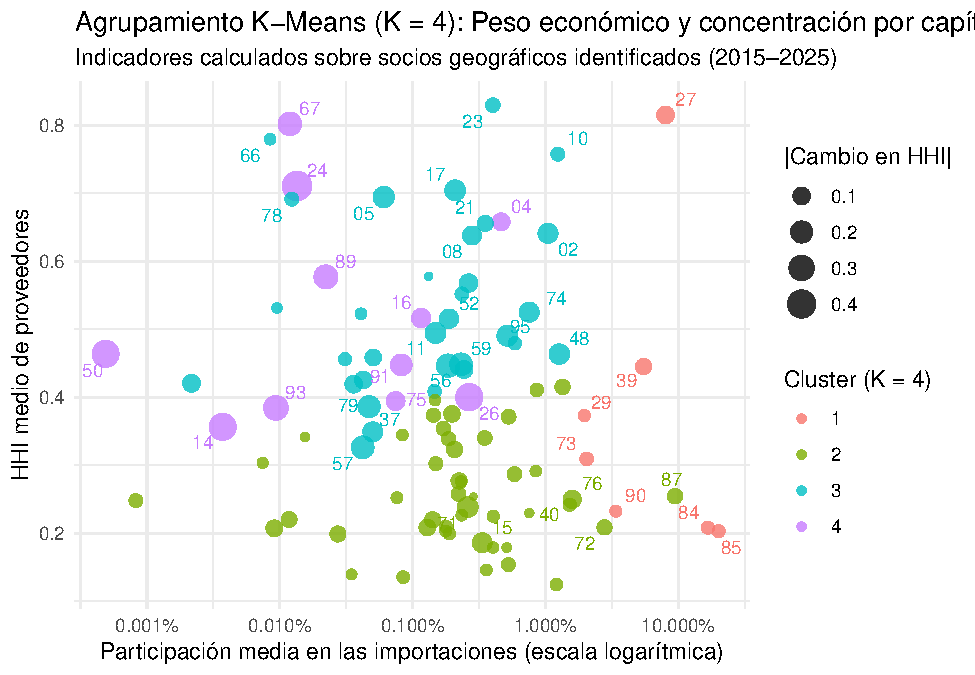
\includegraphics{Proyecto_9_EDA_files/Proyecto_9_EDA_files/figure-latex/unnamed-chunk-23-1.pdf}
En esta gráfica, la línea horizontal punteada en cero separa a los
capítulos que aumentaron su concentración entre 2015--2017 y 2023--2025
(arriba) de aquellos que la redujeron (abajo). Se aprecia que entre los
capítulos de gran peso comercial, maquinaria mecánica (\texttt{84}) y
vehículos (\texttt{87}) se ubican por debajo de cero (disminución del
HHI), mientras que combustibles minerales (\texttt{27}) se ubica por
encima de cero al haber incrementado la proporción del valor concentrado
en su proveedor principal.

\subsubsection{Limitaciones e interpretación de los
resultados}\label{limitaciones-e-interpretaciuxf3n-de-los-resultados}

En la gráfica del Método del Codo se ve que el avance más importante
ocurre al pasar de 2 a 4 grupos. A partir de 5 y hasta 8 grupos la línea
se aplana casi por completo, lo que significa que duplicamos la cantidad
de grupos sin obtener una mejora relevante en el resultado.

El análisis utiliza el valor comercial en dólares corrientes
(\texttt{primaryValue}). Por ello, los cambios observados en la
participación o en el HHI de capítulos como combustibles (\texttt{HS27})
o cereales (\texttt{HS10}) pueden estar influidos por variaciones
internacionales de precios y no reflejan necesariamente cambios
equivalentes en las cantidades físicas importadas.

Como se documentó en la sección de preparación del modelo, en años
recientes aumentó el valor registrado bajo etiquetas que no identifican
a un país específico (particularmente \emph{``Other Asia, nes''}, que
representó 22.45\% del valor de \texttt{HS84} en 2025). Para no cometer
el error de contar esa categoría general como si fuera un solo país
vendedor, el modelo se calculó únicamente con las compras donde sí se
conoce el país de procedencia. Por ello, los grupos obtenidos muestran
cómo se reparte el comercio solo entre los países identificados

Los códigos de dos dígitos (HS2) reúnen sectores completos (como toda la
electrónica o todos los vehículos) y no productos individuales. Por eso,
aunque un sector completo tenga sus compras bien repartidas entre varios
países, dentro de él todavía pueden existir productos muy específicos (a
nivel de cuatro o seis dígitos) que dependan de un solo proveedor.
Además, estos números reflejan cómo se distribuye el dinero de las
compras, pero no indican qué tan fácil sería cambiar de vendedor en la
práctica ni explican por sí solos las causas de esos cambios.

\subsubsection{Conclusiones}\label{conclusiones}

Al evaluar qué capítulos HS2 de las importaciones mexicanas combinan
mayor importancia económica y concentración de proveedores entre 2015 y
2025, observamos un contraste claro entre las manufacturas principales y
el sector energético y agroalimentario: * Los capítulos de mayor valor
importado ---\textbf{equipo eléctrico (\texttt{HS85})},
\textbf{maquinaria mecánica (\texttt{HS84})} y \textbf{vehículos y
autopartes (\texttt{HS87})}--- mantienen niveles de concentración
moderados o bajos y registraron una disminución en la cuota de su
proveedor principal (Estados Unidos) y en su HHI entre el inicio y el
final del periodo. * En cambio, \textbf{combustibles minerales
(\texttt{HS27})}, junto con capítulos agroalimentarios de valor
relevante como \textbf{cereales (\texttt{HS10})} y \textbf{semillas
oleaginosas (\texttt{HS12})}, combinan una participación importante
dentro de las importaciones con niveles de concentración muy elevados,
mostrando además un aumento del HHI en el caso de los combustibles.

Por otro lado, los resultados son consistentes con la hipótesis
planteada: la concentración de proveedores no cambió de la misma manera
en todos los capítulos. Mientras que una parte amplia de los capítulos
manufactureros intermedios redujo su HHI entre 2015--2017 y 2023--2025,
otros capítulos de alta concentración mantuvieron o incrementaron el
peso de su socio principal.

Por ultimo, aunque el coeficiente \emph{silhouette} promedio alcanzó su
valor máximo en \(K=2\) (\texttt{0.511}), el análisis de perfiles
demostró que dos grupos separan a los capítulos casi exclusivamente por
su escala económica (\texttt{8.27\%} frente a \texttt{0.43\%} de
participación media), dejando niveles de HHI similares en ambos grupos.
Ampliar el agrupamiento a \(K=4\) permitió distinguir perfiles que
separan tanto el peso económico como el nivel y la dirección del cambio
en el HHI.

\end{document}
